%Este trabalho está licenciado sob a Licença Atribuição-CompartilhaIgual 4.0 Internacional Creative Commons. Para visualizar uma cópia desta licença, visite http://creativecommons.org/licenses/by-sa/4.0/deed.pt_BR ou mande uma carta para Creative Commons, PO Box 1866, Mountain View, CA 94042, USA.

\documentclass[a4paper,10pt,twoside]{book}

%%% preambulo
\input ../preambulo.tex
\input ../preambulo_counters.tex
\input ../preambulo_python.tex


\begin{document}

\frontmatter

% título
\title{Algoritmos e Programação I}
\author{Pedro H A Konzen}
\date{}
\maketitle

% ficha catolográfica
\ifisbook
~
\vspace{4.5in}
\hrule
Konzen, Pedro Henrique de Almeida \\
\indent\hspace{2em}Algoritmos e programação I: notas de aula / Pedro Henrique de Almeida Konzen. --{\the\year}. Porto Alegre.- {\the\year}. \\
\indent\hspace{2em}"Esta obra é uma edição independente feita pelo próprio autor." \\
\indent\hspace{2em}1. Algoritmos computacionais. 2. Programação de computadores. 3. Linguagem Python. \\
\hrule
\vspace{1cm}
\begin{center}
  \textit{Licença}\\CC-BY-SA 4.0.
\end{center}
\fi

% licença
%Este trabalho está licenciado sob a Licença Atribuição-CompartilhaIgual 4.0 Internacional Creative Commons. Para visualizar uma cópia desta licença, visite http://creativecommons.org/licenses/by-sa/4.0/ ou mande uma carta para Creative Commons, PO Box 1866, Mountain View, CA 94042, USA.

\section*{Licença}\label{licenca}
\addcontentsline{toc}{section}{Licença}

Este trabalho está licenciado sob a Licença Atribuição-CompartilhaIgual 4.0 Internacional Creative Commons. Para visualizar uma cópia desta licença, visite http://creativecommons.org/licenses/by-sa/4.0/deed.pt\_BR ou mande uma carta para Creative Commons, PO Box 1866, Mountain View, CA 94042, USA.


% prefácio


\chapter*{Prefácio}\label{prefacio}
\addcontentsline{toc}{chapter}{Prefácio}

O site \href{https://www.notaspedrok.com.br}{notaspedrok.com.br} é uma plataforma que construí para o compartilhamento de minhas notas de aula. Essas anotações feitas como preparação de aulas é uma prática comum de professoras/es. Muitas vezes feitas a rabiscos em rascunhos com validade tão curta quanto o momento em que são concebidas, outras vezes, com capricho de um diário guardado a sete chaves. Notas de aula também são feitas por estudantes - são anotações, fotos, prints, entre outras formas de registros de partes dessas mesmas aulas. Essa dispersão de material didático sempre me intrigou e foi o que me motivou a iniciar o site.

Com início em 2018, o site contava com apenas três notas incipientes. De lá para cá, conforme fui expandido e revisando os materiais, o site foi ganhando acessos de vários locais do mundo, em especial, de países de língua portuguesa. No momento, conta com 13 notas de aula, além de minicursos e uma coleção de vídeos e áudios.

As notas de \emph{Matemática Numérica III} abordam tópicos sobre sistemas lineares de médio/grande porte, sistemas não-lineares, problemas de otimização, problemas de autovalores e integração auto-adaptativa. Códigos exemplos são apresentados em linguagem {\python}.

Aproveito para agradecer a todas/os que de forma assídua ou esporádica contribuem com correções, sugestões e críticas! ;)

\begin{flushright}
  Pedro H A Konzen

  \url{https://www.notaspedrok.com.br}
\end{flushright}

% toc
\ifishtml
\clearpage
\phantomsection
\addcontentsline{toc}{chapter}{Conteúdo}
\fi
\tableofcontents


\mainmatter



\chapter{Introdução}\label{cap_intro}
\thispagestyle{fancy}

\emconstrucao
\chapter{Linguagem de Programação}\label{cap_lingua}

\section{Computador}\label{cap_lim_sec_computador}

\hl{Um computador é um \emph{sistema computacional} de elementos físicos (\emph{hardware}) e elementos lógicos (\emph{software})}.

\hl{O \emph{hardware} são suas partes mecânicas, elétricas e eletrônicas} como: fonte de energia, teclado, mouse/painel tátil, monitor/tela, dispositivos de armazenagem de dados (HDD, \textit{hard disk drive}; SSD, \textit{solid-state drive}; RAM, \textit{random-access memory}; etc.), dispositivos de processamento (CPU, \textit{central processing unit}, GPU, \textit{graphics processing unit}), conectores de dispositivos externos (microfone, caixa de som, fone de ouvido, USB, etc.), placa mãe, etc..

\hl{O \emph{software} é toda a informação processada pelo computador}, qualquer código executado e qualquer dado usado nas computações.

\begin{figure}[htb]
  \centering
  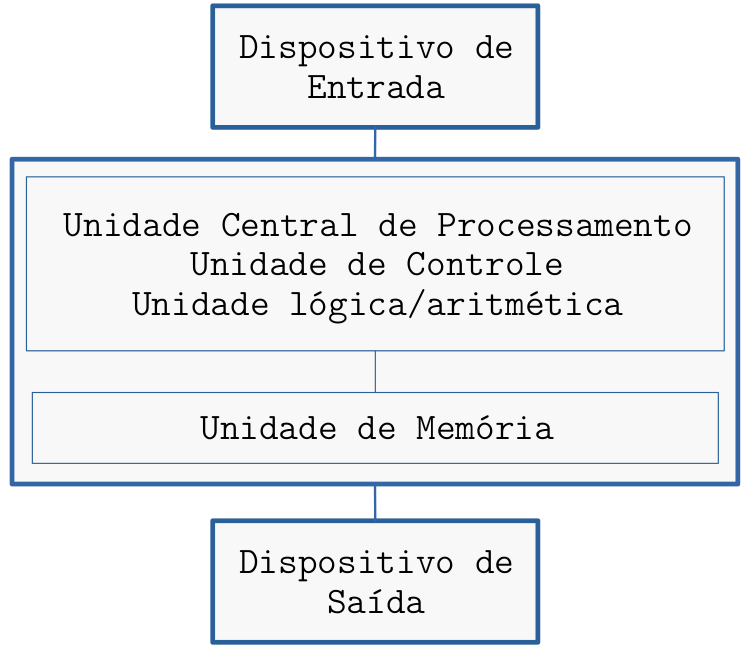
\includegraphics[width=2.5in]{./cap_lingua/dados/fig_arqVonNeumann/fig.png}
  \caption[Arquitetura de von Neumann]{Arquitetura de computador de von Neumann.}
  \label{cap_lim_sec_computador:fig:arqVonNeumann}
\end{figure}

Os computadores que comumente utilizamos seguem a arquitetura de John von Neumann{\vonNeumann}, que consiste em dispositivo(s) de entrada de dados, unidade(s) de processamento, unidade(s) de memória e dispositivo(s) de saída de dados (Figura~\ref{cap_lim_sec_computador:fig:arqVonNeumann}).

\begin{itemize}
\item \hlemph{Dispositivos de entrada e saída}

  São elementos do computador que permitem a comunicação humana (usuária(o)) com a máquina.

  \begin{itemize}
  \item \hlemph{Dispositivos de entrada}

    São elementos que permitem o fluxo de informação da(o) usuária(o) para a máquina. Exemplos são: teclado, mouse/painel tátil, microfone, etc.

  \item \hlemph{Dispositivos de saída}

    São elementos que permitem o fluxo de informação da máquina para a(o) usuária(o). Exemplos são: monitor/tela, alto-falantes, luzes espia, etc.
  \end{itemize}

\item \hlemph{Unidade central de processamento}

  A \emph{CPU} (do inglês, \textit{Central Processing Unit}) é o elemento que processa as informações e é composta de \emph{unidade de controle}, \emph{unidade lógica e aritmética} e de \emph{memória cache}.

  \begin{itemize}
  \item \hlemph{Unidade de controle}

    Coordena as execuções do processador: busca e decodifica instruções, lê e escreve no \textit{cache} e controla o fluxo de dados.

  \item \hlemph{Unidade lógica/aritmética}

    Executa as instruções operações lógicas e aritméticas, por exemplo: executar a adição, multiplicação, testar se dois objetos são iguais, etc.

  \item \hlemph{Memória cache}

    Memória interna da CPU muito mais rápida que as memórias RAM e dispositivos e armazenamento HDD/SSD. É um dispositivo de memória de pequena capacidade e é utilizada como memória de curto prazo e diretamente acessada.
  \end{itemize}

\item \hlemph{Unidades de memória}

  As unidades de memória são elementos que permitem o armazenamento de dados/objetos. Como memória principal tem-se a \emph{ROM} (do inglês, \textit{Read Only Memory}) e a \emph{RAM} (do inglês, \textit{Random Access Memory}) e como memória de massa/secundária tem-se HDD, SSD, entre outras.

\item \hlemph{Memória ROM}

  A memória ROM é utilizada para armazenamento de dados/objetos necessários para dar início ao funcionamento do computador. Por exemplo, é onde a BIOS (dos inglês, \textit{Basic Input/Output System}, Sistema Básico de Entrada e Saída) é armazenada. Ao ligarmos o computador este programa é iniciado e é responsável por fazer o gerenciamento inicial dos diversos dispositivos do computador e carregar o \emph{sistema operacional} (conjunto de programas cuja função é de gerenciar os recursos do computador e controlar a execução de programas).

\item \hlemph{Memória RAM}

  Memória de acesso rápido utilizada para dados/objetos de uso frequente durante a execução de programas. É uma memória volátil, i.e. toda a informação guardada nela é perdida quando o computador é desligado.

\item \hlemph{Memória de massa/secundária}

  Memória de massa ou secundária são usadas para armazenar dados/objetos por período longo. Normalmente, são dispositivos HDD ou SSD, os dados/objetos são guardados mesmo que o computador seja desligado e contém grande capacidade de armazenagem.   
\end{itemize}

\hl{Os \emph{software} são os elementos lógicos de um sistema computacional, são programas de computadores que contém as instruções que gerenciam o \emph{hardware} para a execução de tarefas específicas}, por exemplo, imprimir um texto, gravar áudio/vídeo, resolver um problema matemático, etc. Programar é o ato de criar programas de computadores.

\subsection{Linguagem de Programação}

\hl{As informações fluem no computador codificadas como registros de \textit{bits}}\endnote{Usualmente, de tamanho $64$-\textit{bits}.}\hl{ (sequência de zeros ou uns)}. Há registros de instrução e de dados. Programar diretamente por registros é uma tarefa muito difícil, o que levou ao surgimento de linguagens de programação. \hl{Uma \emph{linguagem de programação}}\endnote{Código de programação, código de máquina ou linguagem de máquina.}\hl{ é um método padronizado para escrever instruções para execução de tarefas no computador}. As instruções escritas em uma linguagem são interpretadas e/ou compiladas por um software (interpretador ou compilador) da linguagem que decodifica as instruções em registros de instruções e dados, os quais são efetivamente executados na máquina.

Existem várias linguagens de programação disponíveis e elas são classificadas por diferentes características. Uma \emph{linguagem de baixo nível} (por exemplo, \href{https://pt.wikipedia.org/wiki/Linguagem_assembly}{Assembly}) é aquela que se restringe às instruções executadas diretamente pelo processador, enquanto que uma \emph{linguagem de alto nível} contém instruções mais complexas e abstratas. Estas contém sintaxe mais próxima da linguagem humana natural e permitem a manipulação de objetos mais abstratos. Exemplos de linguagens de alto nível são: \href{https://pt.wikipedia.org/wiki/BASIC}{Basic}, \href{https://pt.wikipedia.org/wiki/Java\_(linguagem\_de\_programa\%C3\%A7\%C3\%A3o)}{Java}, \href{https://pt.wikipedia.org/wiki/JavaScript}{Javascript}, \href{https://pt.wikipedia.org/wiki/MATLAB}{MATLAB}, \href{https://pt.wikipedia.org/wiki/PHP}{PHP}, \href{https://pt.wikipedia.org/wiki/R\_(linguagem_de_programa\%C3\%A7\%C3\%A3o)}{R}, \href{https://pt.wikipedia.org/wiki/C\%2B\%2B}{C/C++}, {\python}, etc.

\hl{Em geral, não existe uma melhor linguagem, cada uma tem suas características que podem ser mais ou menos adequadas conforme o programa que se deseja desenvolver}. Por exemplo, para um site de internet, linguagens como \href{https://pt.wikipedia.org/wiki/JavaScript}{Javascript} e \href{https://pt.wikipedia.org/wiki/PHP}{PHP} são bastante úteis, mas não no desenvolvimento de modelagem matemática e computacional. Nestes casos, \href{https://pt.wikipedia.org/wiki/C\%2B\%2B}{C/C++} é uma linguagem mais apropriada por conter várias estruturas de programação que facilitam a modelagem computacional de problemas científicos. Agora, \href{https://pt.wikipedia.org/wiki/R\_(linguagem_de_programa\%C3\%A7\%C3\%A3o)}{R} é uma linguagem de alto nível com diversos recursos dedicados às áreas de ciências de dados e estatística. Usualmente, utiliza-se mais de uma linguagem no desenvolvimento de programas mais avançados. A ideia é de explorar o melhor de cada linguagem na criação de programas eficientes na resolução dos problemas de interesse.

Nestas notas de aula, \hl{{\python}} é a linguagem escolhida para estudarmos algoritmos e programação. Trata-se de uma \hl{linguagem de alto nível, \emph{interpretada}, \emph{dinâmica} e \emph{mutiparadigma}}. Foi lançada por Guido van Rossum{\rossum} em 1991 e, atualmente, é desenvolvida de forma comunitária, aberta e gerenciada pela ONG \href{https://pt.wikipedia.org/wiki/Python_Software_Foundation}{Python Software Foundation}. A linguagem foi projetada para priorizar a legibilidade do código. Parte da filosofia da linguagem é descrita pelo poema \href{https://pt.wikipedia.org/wiki/Zen_de_Python}{The Zen of Python}. Pode-se lê-lo pelo \textit{easter egg} {\python}

\begin{lstlisting}
import this
\end{lstlisting}

Verifique!

\begin{itemize}
\item \hlemph{Linguagem interpretada}

  {\python} é uma linguagem interpretada. Isso significa que o \emph{código-fonte} escrito em linguagem {\python} é interpretado por um programa (interpretador {\python}). Ao executar-se um código, o interpretador lê uma linha do código, decodifica-a como registros para o processador que os executa. Executada uma linha, o interpretador segue para a próxima até o código ter sido completadamente executado.

\item \hlemph{Linguagem compilada}

  Em uma linguagem compilada, como \href{https://pt.wikipedia.org/wiki/C\%2B\%2B}{C/C++}, há um programa chamado de \emph{compilador} (em inglês, \textit{compiler}) e outro de \emph{ligador} (em inglês, \textit{linker}). O primeiro, cria um programa-objeto a partir do código e o segundo gerencia sua ligação com eventuais bibliotecas computacionais que ele possa depender. O programa-objeto (também chamado de executável) pode então ser executado pela máquina.
\end{itemize}

Em geral, a execução de um programa compilado é mais rápida que a de um código interpretado. De forma simples, isso se deve ao fato de que nesse a interpretação é feita toda de uma vez e não precisa ser refeita na execução de cada linha de código, como no segundo caso. Por outro lado, a compilação de códigos-fonte grandes pode ser bastante demorada fazendo mais sentido quando ele é compilado uma vez e o programa-objeto executado várias vezes. Além disso, linguagens interpretadas podem usar bibliotecas de programas pré-compiladas. Com isso, pode-se alcançar um bom balanceamento entre tempo de desenvolvimento e de execução do código.

O interpretador {\python} também pode ser usado para compilar o código para um arquivo \emph{bytecode}, este é executado muito mais rápido do que o código-fonte em si, pois as interpretações necessárias já foram feitas. Mais adiante, vamos estudar isso de forma mais detalhada.

\ifisbook
\newpage
\fi

\begin{itemize}
\item \hlemph{Linguagem de tipagem dinâmica}

  {\python} é uma linguagem de tipagem dinâmica. Nela, os dados não precisam ser explicitamente tipificados no código-fonte e o interpretador os tipifica com base em regras da própria linguagem. Ao executar operações com os dados, o interpretador pode alterar seus tipos de forma dinâmica.

\item \hlemph{Linguagem de tipagem estática}

  \href{https://pt.wikipedia.org/wiki/C\%2B\%2B}{C/C++} é um exemplo de uma linguagem de tipagem estática. Em tais linguagens, os dados devem ser explicitamente tipificados no código-fonte com base nos tipos disponíveis. A retipificação pode ocorrer, mas precisa estar explicitamente definida no código.
\end{itemize}

Existem vários \emph{paradigmas de programação} e a \hl{linguagem {\python} é multiparadigma}, i.e. permite a utilização de mais de um no código-fonte. Exemplos de paradigmas de programação são: \emph{estruturada}, \emph{orientada a objetos}, \emph{orientada a eventos}, etc.. Na maior parte destas notas de aulas, vamos estudar algoritmos para linguagens de programação estruturada. Mais ao final, vamos introduzir aspectos de linguagens orientada a objetos. Estes são paradigmas de programação fundamentais e suas estruturas são importantes na programação com demais paradigmas disponíveis em programação de computadores.

\subsection{Instalação e Execução}

\hl{{\python} é um \emph{software aberto}}\endnote{Consulte a licença de uso em \url{https://docs.python.org/3/license.html}.} e está disponível para vários sistemas operacionais ({\linux}, macOS, Windows, etc.) no seu site oficial
\begin{center}
  \url{https://www.python.org/}
\end{center}
Também, está disponível (gratuitamente) na loja de aplicativos dos sistemas operacionais mais usados. Esta costuma ser a forma mais fácil de instalá-lo na sua máquina, consulte a loja de seus sistema operacional. Ainda, há plataformas e IDEs\endnote{IDE, do inglês, \textit{integrated development environment}, ambiente de desenvolvimento integrado} {\python} disponíveis, consulte, como por exemplo, \href{https://www.anaconda.com/}{Anaconda}.

A execução de um código {\python} pode ser feita de várias formas.

\begin{itemize}
\item \hlemph{Execução iterativa via terminal}

  Em terminal {\python} pode-se executar instruções/comandos de forma iterativa. Por exemplo:

\begin{lstlisting}[xrightmargin=2.5em]
>>> print('Olá, mundo!')
Olá, mundo!
>>> 
\end{lstlisting}      

  \hl{O símbolo }\lstinline+>>>+\hl{ denota o \emph{prompt de entrada}, onde uma instrução {\python} pode ser digitada}. Após digitar, o comando é executada teclando \lstinline+<ENTER>+. Caso o comando tenha alguma \hl{saída de dados}, como no caso acima, esta aparecerá, por padrão, \hl{no \emph{prompt de saída}}, logo abaixo a linha de comando executada. \hl{Um novo símbolo de prompt de entrada aparece ao término da execução anterior}.

\item \hlemph{Execução de um \textit{script}}

  Para códigos com várias linhas de instruções é mais adequado utilizar um aquivo de \textit{script} {\python}. Usando-se um editor de texto ou um IDE ditam-se as linhas de comando em um arquivo \lstinline+.py+. Então, \textit{script} pode ser executado em um terminal de seu sistema operacional utilizando-se o interpretador {\python}. Por exemplo, assumindo que o código for salvo do arquivo \lstinline+path_to_arq/arq.py+, pode-se executá-lo em um terminal do sistema com

\begin{lstlisting}[xrightmargin=2.5em]
$ python3 path_to_arq/arq.py 
\end{lstlisting}%$
  

  IDEs para {\python} fornecem uma ambiente integrado, contendo um campo para escrita do código e terminal {\python} integrado. Consulte, por exemplo, o IDE {\spyder}:
  \begin{center}
    \url{https://www.spyder-ide.org/}
  \end{center}

\item \hlemph{Execução em um \textit{notebook}}

  \textit{Notebooks} {\python} são uma boa alternativa para a execução de códigos em um ambiente colaborativo/educativo. Por exemplo, {\jupyter} é um notebook que roda em navegadores de internet. Sua estrutura e soluções também são encontradas em notebooks online (de uso gratuito limitado) como {\colab} e {\kaggle}. Em \texttt{notebooks} as instruções/comandos são organizados em células de código.

  Ao longo dessas notas, vamos assumir que os códigos são implementados em um \texttt{notebook}. Uma célula de código é apresentada com suas linhas enumeradas como, por exemplo,

\begin{lstlisting}[xrightmargin=2.5em]
print('Olá, mundo!')  
\end{lstlisting}

E, quando for o caso, a saída aparece logo abaixo como, no caso,

\begin{verbatim}
Olá, mundo!
\end{verbatim}

\end{itemize}

\subsection{Exercícios}

% exercícios de compreensão

\begin{exer}
  Complete as lacunas.
  \begin{enumerate}[a)]
    \item \underline{\phantom{\textit{Hardware}}} é um elemento físico de um computador.
    \item \textit{Software} é um elemento \underline{\phantom{lógico}} de um computador.
    \item Teclado e \textit{mouse} são exemplos de dispositivos de \underline{\phantom{entrada}} de dados em um computador.
    \item Monitor/tela e auto-falantes são exemplos de \underline{\phantom{dispositivos de saída}} de dados em um computador.
    \item \underline{\phantom{CPU}} é um dos elementos que processa as informações em um computador.
    \item As \underline{\phantom{unidades de memória}} são elementos que permitem o armazenamento de dados/objetos.
  \end{enumerate}
\end{exer}
\begin{resp}
  a) \textit{Hardware}; b) lógico; c) entrada; d) dispositivos de saída; e) CPU; f) unidades de memória.
\end{resp}

\begin{exer}
  Complete as lacunas.
  \begin{enumerate}[a)]
    \item Uma linguagem de programação é um método para escrever instruções para a execução de \underline{\phantom{tarefas}} no computador.
    \item {\python} é uma linguagem de \underline{\phantom{alto}} nível, de tipagem \underline{\phantom{dinâmica}} e multiparadigma.
  \end{enumerate}
\end{exer}
\begin{resp}
  a) tarefas; b) alto; dinâmica
\end{resp}

% exercícios

\begin{exer}
  Verifique qual a versão do sistema operacional que está utilizado em seu computador.
\end{exer}
\begin{resp}
  Dica: no seu sistema operacional, busque pelas informações do sistema.
\end{resp}

\begin{exer}
  Verifique os seguintes elementos de seu computador:
  \begin{enumerate}[a)]
  \item CPUs
  \item Placa(s) gráfica(s)
  \item Memória RAM
  \item Armazenamento HDD/SSD.
  \end{enumerate}
\end{exer}
\begin{resp}
  Dica: no seu sistema, busque pelas informações do sistema.
\end{resp}

\begin{exer}
  Verifique como entrar na \lstinline+BIOS+ de seu computador. Atenção! Não faça e salve nenhuma alteração. Modificações na \lstinline+BIOS+ podem impedir que seu computador funcione normalmente, inclusive, impedir que você inicialize seu sistema operacional.
\end{exer}
\begin{resp}
  Dica: cada computador tem sua forma de acessar a \lstinline+BIOS+. Verifique o manual ou busque na \textit{web} pela marca e modelo de seu computador.
\end{resp}

\begin{exer}
  Instale {\python} no seu computador (caso ainda não tenha feito) e abra um terminal {\python}. Nele, escreva uma linha de comando que imprime no prompt de saída a frase ``Olá, meu Python!''.
\end{exer}
\begin{resp}

\begin{lstlisting}
>>> print('Olá, meu Python!')
Olá, meu Python!
>>> 
\end{lstlisting}

\end{resp}

\begin{exer}
  Instale um IDE para {\python} no seu computador (caso ainda não tenha feito) e use-o para escrever o seguinte \textit{script}

\begin{lstlisting}
import math as m
print(f'Número pi = {m.pi}')
print(f'Número de Euler e = {m.e}')
\end{lstlisting}

  Também, execute o \textit{script} diretamente em um terminal de seu sistema operacional.
\end{exer}
\begin{resp}
  Dica: instale o IDE {\spyder}, disponível em
  \begin{center}
    \url{https://www.spyder-ide.org/}
  \end{center}
\end{resp}

\begin{exer}
  Use um \textit{notebook} {\python} para escrever e executar o código do exercício anterior.
\end{exer}
\begin{resp}
  Dica: use um notebook online {\colab} (\url{https://colab.research.google.com/}), {\kaggle} (\url{https://www.kaggle.com/}) ou {\jupyter} (\url{https://jupyter.org/}).
\end{resp}

\ifisbook
\subsubsection{Respostas}
\shipoutAnswer
\fi

\section{Algoritmos e Programação}\label{cap_lingua_sec_algoprog}

\hl{\emph{Programar} é criar um programa} (um \textit{software}) \hl{para ser executado em computador}. Para isso, escreve-se \hl{um código em uma linguagem computacional} (por exemplo, em {\python}), o qual é interpretado/compilado para gerar o programa final. \hl{Linguagens computacionais são técnicas, utilizam uma sintaxe simples, precisa e sem ambiguidades}. Ou seja, para criarmos um programa com um determinado objetivo, precisamos escrever um código computacional técnico, que siga a sintaxe da linguagem escolhida e sem ambiguidades.

\hl{Um \emph{algoritmo} pode ser definido uma sequencia ordenada e sem ambiguidade de passos para a resolução de um problema}.

\begin{ex}\label{cap_lingua_sec_algoprog:ex:areaTriang}
O cálculo da área de um triângulo de base e altura dadas por ser feito com o seguinte algoritmo:
\begin{enumerate}
\item Informe o valor da base $b$.
\item Informe o valor da altura $h$.
\item $\displaystyle a \leftarrow \frac{b\cdot h}{2}$.
\item Imprima o valor de $a$.
\end{enumerate}

\hl{Algoritmos para a programação são pensados para serem facilmente transformados em códigos computacionais}. Por exemplo, o algoritmo acima pode ser escrito em {\python} como segue:

\begin{lstlisting}
b = float(input('Informe o valor da base.\n'))
h = float(input('Informe o valor da altura.\n'))
# cálculo da área
a = b*h/2
print(f'Área = {a}')
\end{lstlisting}

\end{ex}

Para criar um programa para resolver um dado problema, começamos desenvolvendo um algoritmo para resolvê-lo, este algoritmo é implementado na linguagem computacional escolhida, a qual gera o programa final. Aqui, o passo mais difícil costuma ser o desenvolvimento do algoritmo. Precisamos pensar em como podemos resolver o problema de interesse em uma sequência de passos ordenada e sem ambiguidades para que possamos implementá-los em computador.

\hl{Um algoritmo deve ter as seguintes propriedades}:
\begin{itemize}
\item \hl{Cada passo deve estar bem definido}, i.e. não pode conter ambiguidades.
\item \hl{Cada passo deve contribuir de forma efetiva na solução do problema}.
\item \hl{Deve ter número finito de passos} que podem ser \hl{computados em um tempo finito}.
\end{itemize}

\begin{obs}\normalfont{(\hl{Mulher na Matemática}.)}
  A primeira pessoa a publicar um algoritmo para programação foi \hl{Augusta Ada King}{\lovelace}. O algoritmo foi criado para computar os \href{https://pt.wikipedia.org/wiki/N\%C3\%BAmeros\_de\_Bernoulli}{números de Bernoulli}{\bernoulli}.
\end{obs}


\subsection{Fluxograma}

\hl{Fluxograma é uma representação gráfica de um algoritmo}. Entre outras, usam-se as seguintes formas para representar tipos de ações a serem executadas:

\begin{itemize}
\item \hlemph{Terminal}: início ou final do algoritmo.
  \begin{center}
    
\includegraphics[width=0.75in]{./cap_lingua/dados/fig_fluxograma/terminal.png}
  \end{center}  
\item \hlemph{Linha de fluxo}: direciona para a próxima execução.
  \begin{center}
    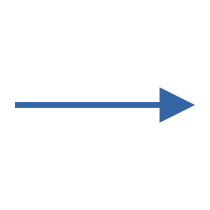
\includegraphics[width=0.75in]{./cap_lingua/dados/fig_fluxograma/linha.png}
  \end{center}
\item \hlemph{Entrada}: leitura de informação/dados.
  \begin{center}
    
\includegraphics[width=0.75in]{./cap_lingua/dados/fig_fluxograma/entrada.png}
  \end{center}  
\item \hlemph{Processo}: ação a ser executada.
  \begin{center}
    
\includegraphics[width=0.75in]{./cap_lingua/dados/fig_fluxograma/processo.png}
  \end{center}
\item \hlemph{Decisão}: ramificação do processamento baseada em uma condição.
  \begin{center}
    
\includegraphics[width=0.75in]{./cap_lingua/dados/fig_fluxograma/decisao.png}
  \end{center}
\item \hlemph{Saída}: impressão de informação/dados.
  \begin{center}
    
\includegraphics[width=0.75in]{./cap_lingua/dados/fig_fluxograma/saida.png}
\end{center}
\end{itemize}

\begin{ex}\label{cap_lingua_sec_algoprog:ex:metHeron}
  O \href{https://en.wikipedia.org/wiki/Methods_of_computing_square_roots#Heron's_method}{método de Heron}{\heron} é um algoritmo para o cálculo aproximado da raiz quadrada de um dado número $x$, i.e. $\sqrt{x}$. Consiste na iteração
  \begin{align}
    & s^{(0)} = \text{approx. inicial},\\
    & s^{(i+1)} = \frac{1}{2}\left(s^{(i)} + \frac{x}{s^{(i)}}\right),
  \end{align}
  para $i=0,1,2,\ldots,n$, onde $n$ é o número de iterações calculadas.

  Na sequência, temos um algoritmo e seus fluxograma e código {\python} para computar a quarta aproximação de $\sqrt{x}$, assumindo $s^{(0)} = x/2$ como aproximação inicial.

  \begin{itemize}
  \item \emph{Algoritmo}
    \begin{enumerate}
    \item Entre o valor de $x$.
    \item Se $x\geq 0$, faça:
      \begin{enumerate}
      \item $s \leftarrow x/2$
      \item Para $i = 0,1,2,3$, faça:
        \begin{enumerate}
        \item $s \leftarrow (s + x/s)/2$.
        \end{enumerate}
      \item Imprime o valor de $s$.
      \end{enumerate}
    \item Senão, faça:
      \begin{enumerate}
      \item Imprime mensagem ``Não existe!''.
      \end{enumerate}
    \end{enumerate}

  \item \emph{Fluxograma}
  
    Consulte a Figura~\ref{cap_lingua_sec_algoprog:fig:metHeron}.  

    \begin{figure}[!hp]
      \centering
      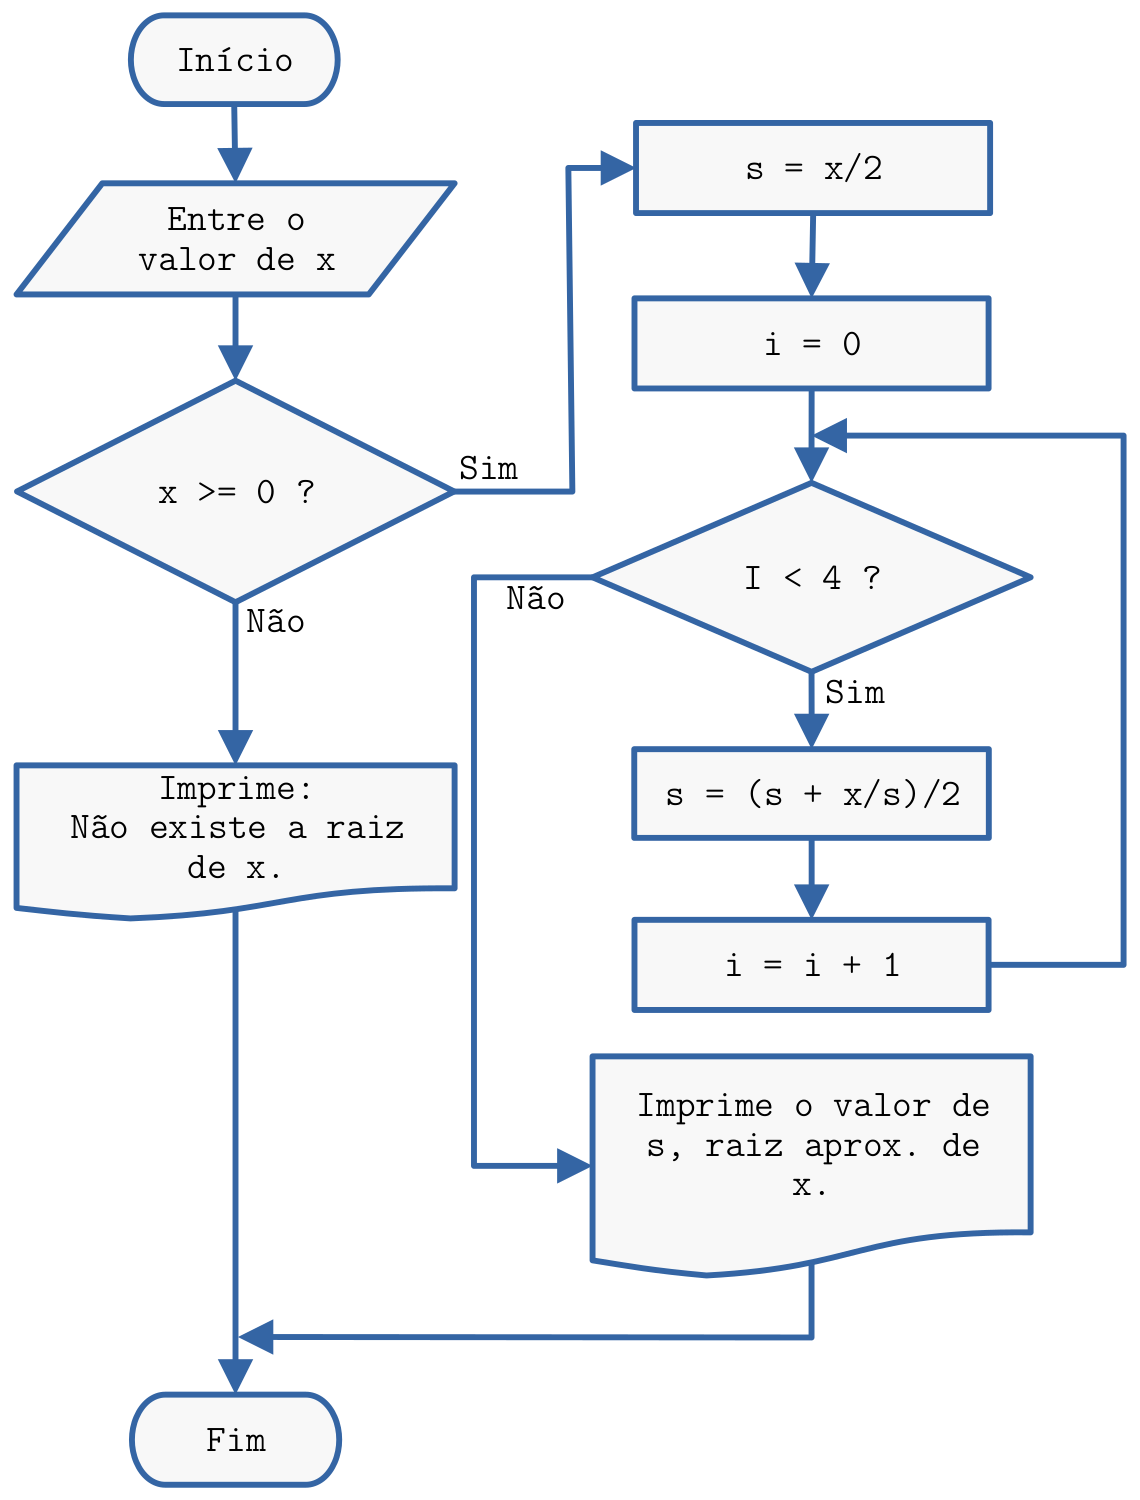
\includegraphics[width=3.8in]{./cap_lingua/dados/fig_fluxograma/fig.png}
      \caption{Fluxograma referente ao Exemplo~\ref{cap_lingua_sec_algoprog:ex:metHeron}.}
      \label{cap_lingua_sec_algoprog:fig:metHeron}
    \end{figure}
  
  \newpage    
  \item \emph{Código {\python}}

\begin{lstlisting}[caption=metHeron.py,label=cap_lingua_sec_algoprog:cod:metHeron, xrightmargin=2.5em]
x = float(input('Entre com o valor de x: '))
if (x >= 0.):
  s = x/2
  for i in range(4):
      s = (s + x/s)/2
  print(f'Raiz aprox. de x = {s}')
else:
  print(f'Não existe!')
\end{lstlisting}

  \end{itemize}

  O algoritmo tem um \textit{bug} (um erro)! Consulte o Exercício~\exerref{cap_lingua_sec_algoprog:exer:bugHeron}.
\end{ex}

\hl{Algoritmos escritos em uma forma próxima de uma linguagem computacional} são, também, chamados de \hl{\emph{pseudocódigos}}. Na prática, pseudocódigos e fluxogramas são usados para apresentar uma forma mais geral e menos detalhada de um algoritmo. Usualmente, sua forma detalhada é escrita diretamente em uma linguagem computacional escolhida.

\subsection{Exercícios}

\begin{exer}
  Complete as lacunas.
  \begin{enumerate}[a)]
    \item Programar é desenvolver um \underline{\phantom{\textit{software}}} para ser executado em um computador.
    \item Linguagens computacionais tem uma \underline{\phantom{sintaxe}} simples, precisa e sem ambiguidades.
    \item Um algoritmo é uma sequência finita de passos \underline{\phantom{bem definidos}} que permitem a resolução \underline{\phantom{objetiva}} de um problema em tempo \underline{\phantom{finito}}.
    \item \underline{\phantom{Pseudocódigo}} é um algoritmo escrito em uma forma próxima de uma linguagem computacional.
  \end{enumerate}
\end{exer}
\begin{resp}
  a) programa/código/\textit{software}. b) sintaxe. c) bem definidos; objetiva; finito. d) Pseudocódigo.
\end{resp}

\begin{exer}
  Complete as lacunas.
  \begin{enumerate}[a)]
    % a)
    \item \underline{\phantom{Fluxograma}} é uma representação gráfica de um algoritmo.
    % b)
    \item Em um fluxograma, \underline{\phantom{terminal}} indicada o início ou final de um algoritmo.
    % c)
    \item A \underline{\phantom{linha de fluxo}} direciona para o próximo bloco de \underline{\phantom{execução}}.
    % d)
    \item A leitura de dados é indicada por um bloco de \underline{\phantom{entrada}} em um fluxograma.
    % e)
    \item Um bloco de \underline{\phantom{processo}} indica uma ação a ser executada.
    % f)
    \item Uma ramificação do algoritmo é indicada no seu fluxograma por um bloco de \underline{\phantom{decisão}}.
    % g
    \item Em um fluxograma, o bloco de \underline{\phantom{saída}} indica a impressão de um dado.
  \end{enumerate} 
\end{exer}
\begin{resp}
  a) Fluxograma. b) terminal. c) linha de fluxo; execução. d) entrada. e) processo. f) decisão. g) saída.
\end{resp}

\begin{exer}
  Escreva um algoritmo/pseudocódigo e um fluxograma correspondente computar a média aritmética entre dois números $x$ e $y$ dados. Como desafio, tente escrever um código {\python} baseado em seu algoritmo.
\end{exer}
\begin{resp}
  \begin{itemize}
    \item Algoritmo
    
\begin{verbatim}
1. Entre com os valores de x e y
2. m = (x + y)/2
3. Imprime m
\end{verbatim}

    \item Fluxograma

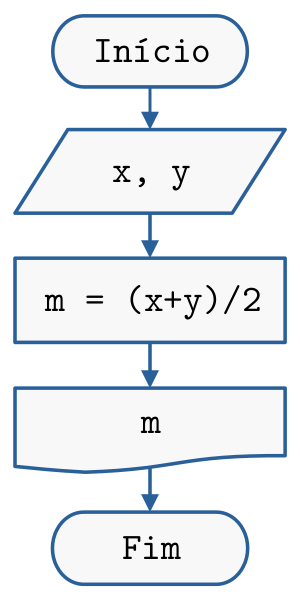
\includegraphics[width=1in]{./cap_lingua/dados/fig_resp_media/fig.png}

  \end{itemize}
\end{resp}

\begin{exer}
  Escreva um algoritmo/pseudocódigo e um fluxograma correspondente para computar a área de um quadrado de lado $l$ dado. Como desafio, tente escrever um código {\python} baseado em seu algoritmo.
\end{exer}
\begin{resp}
  \begin{itemize}
    \item Algoritmo

\begin{verbatim}
1. Entre com o valor de l
2. area = l*l
3. Imprime area
\end{verbatim}

  \end{itemize}
\end{resp}

\begin{exer}
  Escreva um algoritmo/pseudocódigo e um fluxograma correspondente para computar a área de um retângulo de lados $a, b$ dados. Como desafio, tente escrever um código {\python} baseado em seu algoritmo.
\end{exer}
\begin{resp}

\begin{verbatim}
1. Entre com o valor de a
2. Entre com o valor de b
3. area = a*b
4. Imprime area
\end{verbatim}

\end{resp}


\begin{exer}
  Escreva um algoritmo/pseudocódigo e um fluxograma correspondente para computar a área de um triângulo retângulo de dada hipotenusa $h$ e um dos lados $l$ dado. Como desafio, tente escrever um código {\python} baseado em seu algoritmo.
\end{exer}
\begin{resp}
  \begin{itemize}
    \item Algoritmo

\begin{verbatim}
1. Entre com o valor de h
2. Entre com o valor de l
#  o outro cateto
3. m = sqrt(h*h - l*l)
4. area = m*l/2.
5. Imprime area
\end{verbatim}

\item Fluxograma

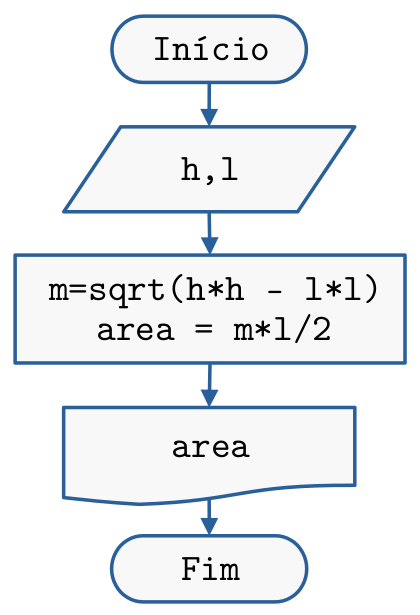
\includegraphics[width=1.4in]{./cap_lingua/dados/fig_resp_triaRet/fig.png}

  \end{itemize}
\end{resp}

\begin{exer}
  Escreva um algoritmo/pseudocódigo e um fluxograma correspondente para computar o zero de uma função afim
  \begin{equation}
    f(x) = ax + b,
  \end{equation}
  dados os coeficientes $a$ e $b$. Como desafio, tente escrever um código {\python} baseado em seu algoritmo.
\end{exer}
\begin{resp}

\begin{verbatim}
1. Entre com o valor de a
2. Entre com o valor de b
3. x0 = -b/a
4. Imprime x0
\end{verbatim}
  
\end{resp}  

\begin{exer}
  Escreva um algoritmo/pseudocódigo e um fluxograma correspondente para computar as raízes reais de um polinômio quadrático
  \begin{equation}
    p(x) = ax^2 + bx + c,
  \end{equation}
  dados os coeficientes $a$, $b$ e $c$. Como desafio, tente escrever um código {\python} baseado em seu algoritmo.
\end{exer}
\begin{resp}

\begin{verbatim}
1. Entre com o valor de a
2. Entre com o valor de b
3. Entre com o valor de c
#  discriminante
4. delta = b*b - 4.*a*c
#  raízes
5. x1 = (-b - sqrt(delta))/2.
6. x2 = (-b + sqrt(delta))/2.
7. Imprime x1 e x2
\end{verbatim}
  
\end{resp}

\begin{exer}
  A \href{https://pt.wikipedia.org/wiki/S%C3%A9rie_harm%C3%B3nica_(matem%C3%A1tica)}{Série Harmônica} é defina por
  \begin{equation}
    \sum_{k=1}^\infty\frac{1}{k} := \frac{1}{1} + \frac{1}{2} + \frac{1}{3} + \cdots
  \end{equation}
  Escreva um algoritmo/pseudocódigo e um fluxograma corresponde para computar o valor da série harmônica truncada em $k=n$, com $n$ dado. Ou seja, dado $n$, o objetivo é calcular
  \begin{equation}
    \sum_{k=1}^n\frac{1}{k} := \frac{1}{1} + \frac{1}{2} + \cdots + \frac{1}{n}.
  \end{equation}
\end{exer}
\begin{resp}
\begin{itemize}
  \item Algoritmo
  
\begin{verbatim}
1. Entre com o valor de n.
2. s = 0.
3. Para i = 1, 2, ... n:
3.1. s = s + 1./i
4. Imprime s
\end{verbatim}

  \item Fluxograma

  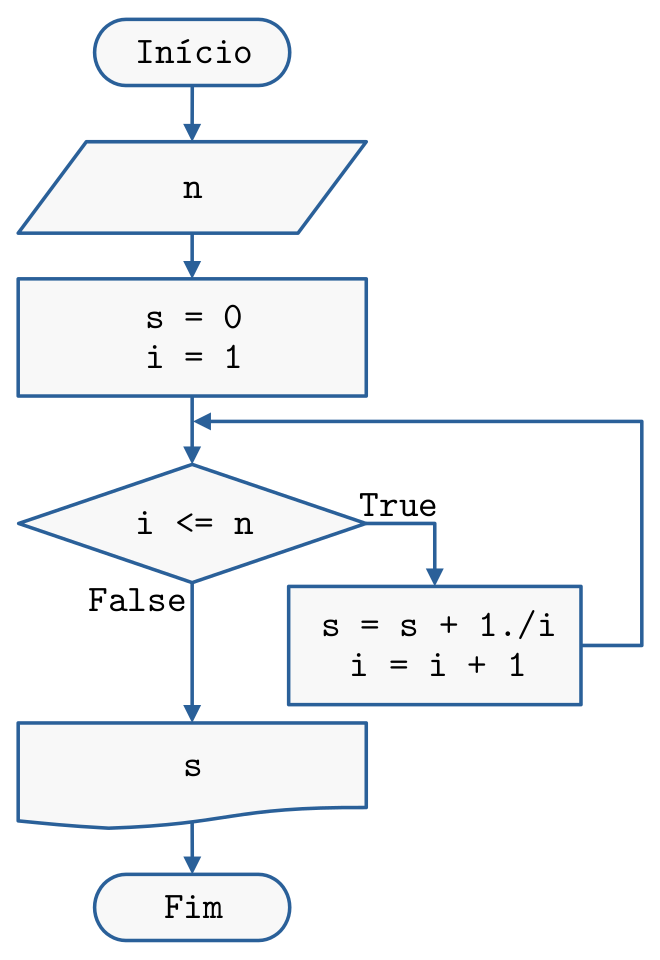
\includegraphics[width=2.2in]{./cap_lingua/dados/fig_resp_serieHarmonica/fig.png}

\end{itemize}
\end{resp}

\begin{exer}

  Escreva um algoritmo/pseudocódigo e um fluxograma corresponde para computar o fatorial de um dado número natural $n$, i.e. computar
  \begin{equation}
    n! = 1\cdot 2\cdot 3 \cdot \cdots \cdot n.
  \end{equation}
\end{exer}
\begin{resp}
  
\begin{verbatim}
1. Entre com o valor de n
2. fat = 1
3. Para i = 2, ..., n:
3.1. fat = fat*i
4. Imprime fat
\end{verbatim}

\end{resp}

\begin{exer}\label{cap_lingua_sec_algoprog:exer:bugHeron}
  O algoritmo construído no Exemplo~\ref{cap_lingua_sec_algoprog:ex:metHeron} tem um \textit{bug} (um erro). Identifique o \textit{bug} e proponha uma nova versão para corrigir o problema. Então, apresente o fluxograma da nova versão do algoritmos. Como desafio, busque implementá-lo em {\python}. 
\end{exer}
\begin{resp}
  Dica: o \textit{bug} ocorre quando $x = 0$.
\end{resp}

\ifisbook
\subsubsection{Respostas}
\shipoutAnswer
\fi

\section{Dados}\label{cap_lingua_sec_dados}

Informação é resultante do processamento, manipulação e organização de \emph{dados} (altura, quantidade, volume, intensidade, densidade, etc.). \hl{Programas de computadores processam, manipulam e organizam \emph{dados computacionais}}. Os dados computacionais são representações em máquina de dados ``reais''. De certa forma, todo dado é uma abstração e, para ser utilizado em um programa de computador, precisa ser representado em máquina.

\hl{Cada dado manipulado em um programa é identificado por um \emph{nome}}, chamado de \hl{\emph{identificador}}. Podem ser variáveis, constantes, funções/métodos, entre outros.
\begin{itemize}
\item \hlemph{Variável}

  Objetos de um programa que armazenam dados que podem mudar de valor durante a sua execução.

\item \hlemph{Constantes}

  Objetos de um programa que não mudam de valor durante a sua execução.

\item \hlemph{Funções e métodos}

  Subprogramas definidos e executados em um programa.
\end{itemize}

\subsection{Identificadores}

\hl{Um identificador é um nome atribuído para a identificação inequívoca de dados que são manipulados em um programa}.

\begin{ex}\label{cap_lingua_sec_dados:ex:reta}
  Vamos desenvolver um programa que computa o ponto de interseção da reta de equação
  \begin{equation}
    y = ax + b
  \end{equation}
  com o eixo $x$ (consulte a Figura~\ref{cap_lingua_sec_dados:fig:ex_reta}).

  \begin{figure}[H]
    \centering
    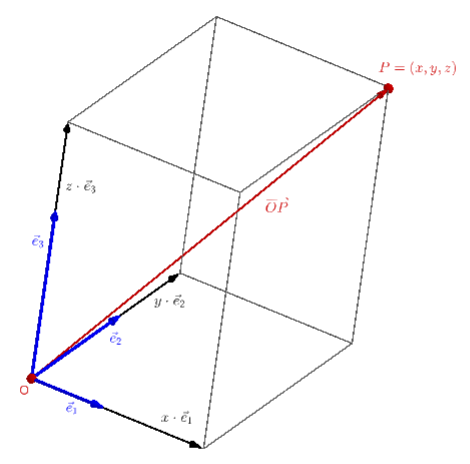
\includegraphics[max width=0.9\textwidth, height=2.75in]{./cap_lingua/dados/fig_ex_reta/fig.png}
    \caption{Esboço da reta de equação $y = ax + b$, com $a=2$ e $b=-1$.}
    \label{cap_lingua_sec_dados:fig:ex_reta}
  \end{figure}

  O ponto $x$ em que a reta intercepta o eixo das abscissas é
  \begin{equation}
    x = -\frac{b}{a}
  \end{equation}
  Assumindo que $a=2$ e $b=-1$, segue um algoritmo para a computação.
  \begin{enumerate}
  \item Atribuir o valor do \emph{coeficiente angular}
    \begin{equation}
      a\leftarrow 2.
    \end{equation}
  \item Atribuir o valor do \emph{coeficiente linear}
    \begin{equation}
      b\leftarrow -1.
    \end{equation}
  \item Computar e armazenar o valor do \emph{ponto de interseção com o eixo $x$}
    \begin{equation}
      x \leftarrow -\frac{b}{a}.
    \end{equation}
  \item Imprimir o valor de $x$.
  \end{enumerate}

  No algoritmo acima, os identificadores utilizados foram: $a$ para o \emph{coeficiente angular}, $b$ para o \emph{coeficiente linear} e $x$ para o \emph{ponto de interseção com o eixo x}.
\end{ex}


\hl{Em {\python}, os identificadores são sensíveis a letras maiúsculas e minúsculas (em inglês, \textit{case sensitive})}, i.e. o identificador \texttt{nome} é diferente dos \texttt{Nome}, \texttt{NoMe} e \texttt{NOME}. Por exemplo:

\begin{lstlisting}
a = 7
print(A)
\end{lstlisting}

\begin{verbatim}
Traceback (most recent call last):
File "<stdin>", line 1, in <module>
NameError: name 'A' is not defined. Did you mean: 'a'?
\end{verbatim}

\hl{Para melhorar a legibilidade de seus códigos, recomenda-se utilizar identificadores com nomes compostos} que ajudem a lembrar o significado do dado a que se referem. No exemplo acima (Exemplo~\ref{cap_lingua_sec_dados:ex:reta}), $a$ representa o \emph{coeficiente angular} da reta e um identificar apropriado seria \texttt{coefAngular} ou \texttt{coef\_angular}.

\hl{Identificadores não podem conter caracteres especiais} (\lstinline+*+, \lstinline+&+, \lstinline+%+,
\lstinline+@+, etc.), \hl{espaços em branco e começar com número}. As seguintes convenções para identificadores com nomes compostos são recomendadas:
\begin{itemize}
\item \hlemph{lowerCamelCase}: \texttt{nomeComposto}
\item \hlemph{UpperCamelCase}: \texttt{NomeComposto}
\item \hlemph{snake}: \texttt{nome\_composto}
\end{itemize}

\begin{obs}\normalfont{(\hl{Identificadores Reservados}.)}
  As seguintes palavras-chave (\texttt{keywords}) são identificadores pré-definidos e reservados:

\begin{verbatim}
  False   await     else     import    pass
  None    break     except   in        raise
  True    class     finally  is        return
  and     continue  for      lambda    try
  as      def       from     nonlocal  while
  assert  del       global   not       with
  async   elif      if       or        yield
\end{verbatim}

\end{obs}

\begin{ex}
  O algoritmo construído no Exemplo~\ref{cap_lingua_sec_dados:ex:reta} pode ser implementado como segue:

\begin{lstlisting}
coefAngular = 2
coefLinear = -1
intercepEixoX = -coefLinear/coefAngular
print(intercepEixoX)
\end{lstlisting}

\end{ex}

\subsection{Alocação de Dados}

Como estudamos acima, \hl{alocamos e referenciamos dados na memória do computador usando identificadores}. Em {\python}, ao executarmos a instrução

\begin{lstlisting}
x = 1
\end{lstlisting}

estamos alocando, na memória do computador, um \emph{objeto} com valor $1$ e \texttt{x} é uma referência para este dado. Pode-se imaginar a memória computacional como um sequência de caixinhas, de forma que \lstinline+x+ será a identificação da caixinha onde o valor $1$ foi alocado.

\begin{center}
  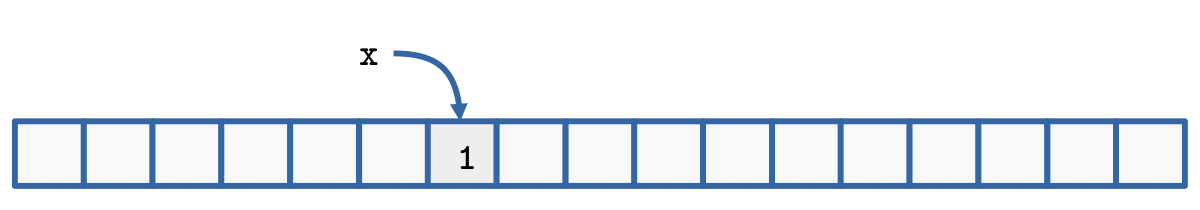
\includegraphics[width=4.5in]{./cap_lingua/dados/fig_aloc_mem/xRecebe1.png}
\end{center}

\hl{Em {\python}, dados têm identidades próprias}. Assim, quando executamos a instrução

\begin{lstlisting}
y = x 
\end{lstlisting}

o identificador \lstinline+y+ passa a referenciar o mesmo local de memória de \lstinline+x+.

\begin{center}
  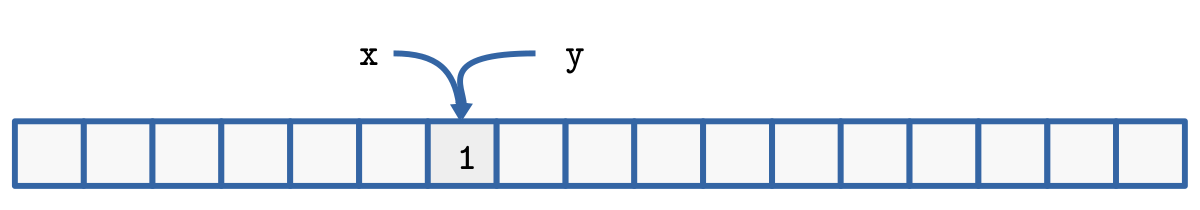
\includegraphics[width=4.5in]{./cap_lingua/dados/fig_aloc_mem/yRecebex.png}
\end{center}

Na sequência, se atribuirmos um novo valor para \lstinline+x+

\begin{lstlisting}
x = 2
\end{lstlisting}

este será alocado em um novo local na memória e \lstinline+x+ passa a referenciar este novo local.

\begin{center}
  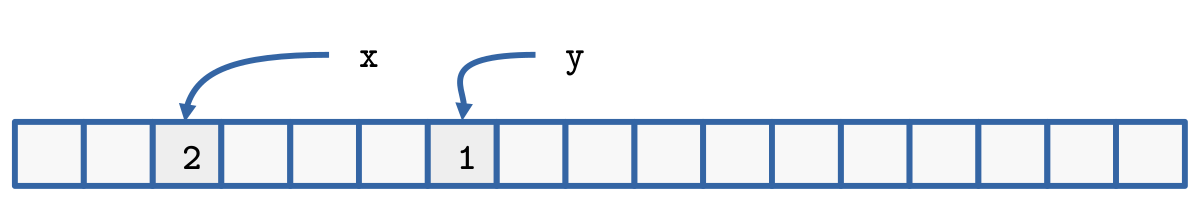
\includegraphics[width=4.5in]{./cap_lingua/dados/fig_aloc_mem/xRecebe2.png}
\end{center}

Ainda, se atribuirmos um novo valor para \lstinline+y+

\begin{lstlisting}
y = 3
\end{lstlisting}

este será alocado em um novo local na memória e \lstinline+y+ passa a referenciar este novo local. O local de memória antigo, em que o valor $1$ está alocado, passa a ficar novamente disponível para o sistema operacional.

\begin{center}
  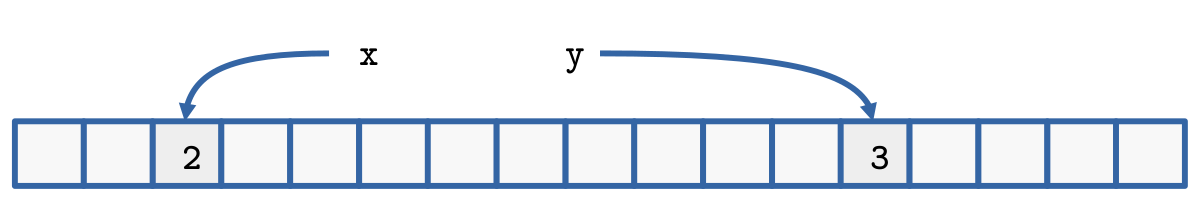
\includegraphics[width=4.5in]{./cap_lingua/dados/fig_aloc_mem/yRecebe3.png}
\end{center}

\begin{obs}
  O método {\python} {\PYTHONid} retorna a identidade de um objeto, seu registro único e constante durante sua alocação no código.

\begin{lstlisting}
x = 1
print('id(x) =', id(x))
\end{lstlisting}

\begin{verbatim}
id(x) = 139779845161200
\end{verbatim}

\begin{lstlisting}
y = x
print('id(y) =', id(y))
\end{lstlisting}

\begin{verbatim}
id(y) = 139779845161200
\end{verbatim}

\begin{lstlisting}
x = 2
print('id(x) =', id(x))
print('id(y) =', id(y))
\end{lstlisting}

\begin{verbatim}
id(x) = 139779845161232
id(y) = 139779845161200
\end{verbatim}

\begin{lstlisting}
y = 3
print('id(y) =', id(y))
\end{lstlisting}

\begin{verbatim}
id(y) = 139779845161264
\end{verbatim}


\end{obs}

\begin{ex}\normalfont{(\hl{Permutação de Variáveis/Identificadores}.)}\label{cap_lingua_sec_dados:ex:trocaVar}
Em várias situações, faz-se necessário permutar dados entre dois identificadores. Sejam

\begin{lstlisting}
x = 1
y = 2
\end{lstlisting}

Agora, queremos permutar os dados, ou seja, queremos que \texttt{y} tenha o valor $1$ e \texttt{x} o valor $2$. Podemos fazer isso utilizando uma variável auxiliar (em inglês, \textit{buffer}).

\begin{lstlisting}
z = x
x = y
y = z
\end{lstlisting}

Verifique!
\end{ex}

\subsection{Exercícios}

\begin{exer}
  Complete as lacunas.
  \begin{enumerate}[a)]
    % a)
    \item Programas de computadores processam, manipulam e organizam \underline{\phantom{dados}}.
    % b)
    \item Um \underline{\phantom{identificador}} é o nome atribuído para a identificação inequívoca de dados em um código computacional.
    % c)
    \item Objetos de um programa que armazenam dados que podem mudar de valor durante a execução do código são chamados de \underline{\phantom{variáveis}}.
    % d)
    \item Objetos que não mudam de valor durante a execução do código são chamados de \underline{\phantom{constantes}}.
    % e)
    \item \underline{\phantom{Função/método}} é um subprograma definido e executado em um programa.
  \end{enumerate}
\end{exer}
\begin{resp}
  a) dados. b) identificador. c) variáveis. d) constantes. e) função/método.
\end{resp}

\begin{exer}
  Proponha identificadores adequados à linguagem {\python} baseados nos seguintes nomes:
  \begin{enumerate}[a)]
  \item Área
  \item Perímetro do quadrado
  \item Cateto+Cateto
  \item Número de elementos do conjunto A
  \item 77 lados
  \item $f(x)$
  \item $x^2$
  \item $13x$
  \end{enumerate}
\end{exer}
\begin{resp}
  a) \lstinline+area+; b) \lstinline+perimetroQuad+; c) \lstinline+somaCatetos+; d) \lstinline+numElemA+; e) \lstinline+lados77+; f) \lstinline+fx+; g) \lstinline+x2+; h) \lstinline+xv13+
\end{resp}

\begin{exer}
  No Exemplo~\ref{cap_lingua_sec_algoprog:ex:areaTriang}, apresentamos um código {\python} para o cálculo da área de um triângulo. Reescreva o código trocando seus identificadores por nomes mais adequados.
\end{exer}
\begin{resp}

\begin{lstlisting}
base = float(input('Informe o valor da base.\n'))
altura = float(input('Informe o valor da altura.\n'))
# cálculo da área
area = base * altura /2
print(f'Área = {area}')
\end{lstlisting}

\end{resp}

\begin{exer}
  O seguinte código {\python} tem um erro/\textit{bug}:

\begin{lstlisting}
x = 1
y = X + 1
\end{lstlisting}

  Identifique-o e apresente uma nova versão do código corrigido.
\end{exer}
\begin{resp}
  Erro: variável \texttt{X} não foi definida.

\begin{lstlisting}
x = 1
y = x + 1
\end{lstlisting}

\end{resp}

\begin{exer}
  Faça uma representação gráfica da alocação de memória que ocorre para cada uma das instruções {\python} que seguem:

\begin{lstlisting}
x = 1
y = 2
z = x
x = y
y = z
\end{lstlisting}

\end{exer}
\begin{resp}

  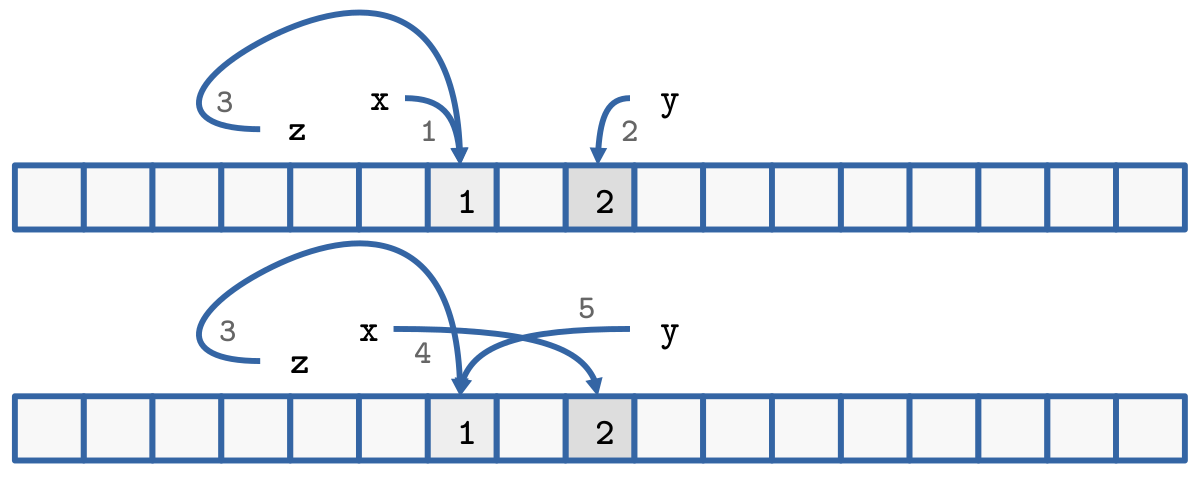
\includegraphics[width=4.5in]{./cap_lingua/dados/fig_aloc_mem/exerPermutacao.jpg}

\end{resp}

\begin{exer}
  No Exemplo~\ref{cap_lingua_sec_dados:ex:trocaVar} fazemos a permutação entre as variáveis \lstinline+x+ e \lstinline+y+ usando um \textit{buffer} \lstinline+z+ para guardar o valor de \lstinline+x+. Se, ao contrário, usarmos o \textit{buffer} para guardar o valor de \lstinline+y+, como fica o código de permutação entre as variáveis?
\end{exer}
\begin{resp}

\begin{lstlisting}
x = 1
y = 2
z = y
y = x
x = z
\end{lstlisting}

\end{resp}

\ifisbook
\subsubsection{Respostas}
\shipoutAnswer
\fi

\section{Dados Numéricos e Operações}\label{cap_lingua_sec_numop}

Números são tipos de dados usualmente manipulados \hl{em programas de computador}. \hl{Números inteiros e não inteiros são tratados de forma diferente}. Mas, antes de discorrermos sobre essas diferenças, vamos estudar operadores numéricos básicos.

\subsubsection{Operações Numéricas Básicas}

As seguintes operações numéricas estão disponíveis na linguagem {\python}:
\begin{itemize}
\item \lstinline*+* \hlemph{adição}

\begin{lstlisting}[xrightmargin=2.5em]
1 + 2
\end{lstlisting}

\begin{verbatim}
3
\end{verbatim}

\item \lstinline+-+ \hlemph{subtração}

\begin{lstlisting}[xrightmargin=2.5em]
1 - 2
\end{lstlisting}

\begin{verbatim}
-1
\end{verbatim}

\item \lstinline+*+ \hlemph{multiplicação}

\begin{lstlisting}[xrightmargin=2.5em]
2*3
\end{lstlisting}

\begin{verbatim}
6
\end{verbatim}

\item \lstinline+/+ \hlemph{divisão}

\begin{lstlisting}[xrightmargin=2.5em]
5/2
\end{lstlisting}

\begin{verbatim}
2.5
\end{verbatim}

\item \lstinline+**+ \hlemph{potenciação}

\begin{lstlisting}[xrightmargin=2.5em]
2**3
\end{lstlisting}

\begin{verbatim}
8
\end{verbatim}

\item \lstinline+//+ \hlemph{divisão inteira}

\begin{lstlisting}[xrightmargin=2.5em]
5//2
\end{lstlisting}

\begin{verbatim}
2
\end{verbatim}

\item \texttt{\%} \hlemph{resto da divisão}

\begin{lstlisting}[xrightmargin=2.5em]
5 % 2
\end{lstlisting}

\begin{verbatim}
1
\end{verbatim}

\end{itemize}

A \hlemph{ordem de precedência das operações} deve ser observada em {\python}. \hl{Uma expressão é executada da esquerda para a direita, mas os operadores tem a seguinte precedência}\endnote{Consulte na \textit{web} a lista completa de operadores e suas precedências em \href{https://docs.python.org/3/reference/expressions.html\#operator-precedence}{The Python Standard Library: Expressions: Operator precedence}.}:

\begin{enumerate}
\item \lstinline+**+
\item \lstinline*-x* (oposto de \texttt{x})
\item \lstinline+*, /, //, %+
\item \lstinline*+, -*
\end{enumerate}

\hl{Utilizamos parênteses para impor uma precedência diferente}, i.e. expressões entre parênteses \lstinline+()+ são executadas antes das demais.

\begin{ex}
  Estudamos a seguinte computação:

\begin{lstlisting}
2+8*3/2**2-1
\end{lstlisting}

\begin{verbatim}
7.0
\end{verbatim}

  Uma pessoa desavisada poderia pensar que o resultado está errado, pois
  \begin{align}
    & 2+8 = 10, \\
    & 10 \cdot 3 = 30, \\
    & 30 \div 2 = 15, \\
    & 15^2 = 225, \\
    & 225 - 1 = 224.
  \end{align}
  Ou seja, o resultado não deveria ser $224$? Não, em {\python}, a operação de potenciação \lstinline+**+ tem a maior precedência, depois vem as de multiplicação \lstinline+*+ e divisão \lstinline+/+ (com a mesma precedência, sendo que a mais a esquerda é executada primeiro) e, por fim, vem as de adição \lstinline*+* e subtração \lstinline+-+ (também com a mesma precedência entre si). Ou seja, a instrução acima é computada na seguinte ordem:
  \begin{align}
    & 2^2 = 4, \\
    & 8\cdot 3 = 24, \\
    & 24\div 4 = 6, \\
    & 2 + 6 = 8, \\
    & 8 - 1 = 7.
  \end{align}

  Para impormos uma ordem diferente de precedência, usamos parêntese. No caso acima, escrevemos

\begin{lstlisting}
((2 + 8)*3/2)**2 - 1
\end{lstlisting}

\begin{verbatim}
224.0
\end{verbatim}

\end{ex}

\begin{obs}\normalfont{(\hl{Espaços entre Operandos}.)}
  O uso de espaços entre os operandos, em geral, é arbitrário, mas conforme utilizados podem dificultar a legibilidade do código. Por exemplo,
\begin{lstlisting}
2 *- 3 + 2
\end{lstlisting}

\begin{verbatim}
-4
\end{verbatim}

  Essa expressão é computada na seguinte ordem
  \begin{align}
    & -~3 = -3 \\
    & 2\cdot(-3) = -6 \\
    & -6 + 2 = -4.
  \end{align}
  Observamos que ela seria melhor escrita da seguinte forma

\begin{lstlisting}
2*-3 + 2
\end{lstlisting}

\begin{verbatim}
-4
\end{verbatim}

\end{obs}

\subsection{Números Inteiros}

\hl{Em {\python}, números inteiros são alocados por registros com um número arbitrário de \textit{bits}}. Com isso, os maior e menor números inteiros que podem ser alocados dependem da capacidade de memória da máquina. \hl{Quanto maior ou menor o número inteiro, mais \textit{bits} são necessários para alocá-lo}.

\begin{ex}
  O método {\python} {\PYTHONsysDOTgetsizeof} retorna o tamanho de um objeto medido em \textit{bytes} \hl{($1~\textit{byte} = 8~\textit{bits}$)}.

\begin{lstlisting}
import sys
print('0:',sys.getsizeof(0),'B')
print('1:',sys.getsizeof(1),'B')
print('100:',sys.getsizeof(100),'B')
print('10**9:',sys.getsizeof(10**9),'B'))
print('10**10:',sys.getsizeof(10**10),'B'))
print('10**100:',sys.getsizeof(10**100),'B'))
\end{lstlisting}

\begin{verbatim}
0: 24 B
1: 28 B
100: 28 B
10**9: 28 B
10**10: 32 B
10**100: 72 B
\end{verbatim}

  O número \href{https://en.wikipedia.org/wiki/Googol}{googol} $10^{100}$ é um número grande\endnote{Por exemplo, o número total de partículas elementares em todo o universo observável é estimado em $10^{80}$. Fonte: \href{https://en.wikipedia.org/wiki/Eddington_number}{Wikipedia: Eddington number}.}, mas $72$~\textit{bytes} não necessariamente. Um computador com $4$~Gbytes\endnote{$1~\textit{Gbytes} = 1024~\textit{Mbytes}$, $1~\textit{Mbytes} = 1024~\textit{Kbytes}$, $1~\textit{Kbytes} = 1024~\textit{bytes}$.} livres de memória, poderia armazenar um número inteiro que requer um registro de até $4,3\times 10^9~\textit{bytes}$.
\end{ex}

\begin{obs}
  O método {\python} {\PYTHONtype} retorna o tipo de objeto alocado. Números inteiros são objetos da classe {\PYTHONint}.

\begin{lstlisting}
type(10)
\end{lstlisting}

\begin{verbatim}
<class 'int'>
\end{verbatim}

\end{obs}

\subsection{Números Decimais}\label{cap_lingua_sec_numop:subsec:float}

No {\python}, \hl{números decimais são alocados} pelo padrão \href{https://en.wikipedia.org/wiki/IEEE\_754}{IEEE 774} de aritmética \hl{em ponto flutuante}. Em geral, são usados $64~\textit{bits} = 8~\textit{bytes}$ para alocar um número decimal. Um ponto flutuante tem a forma
\begin{equation}\hleq
  x = \pm m\cdot 2^{c-1023},
\end{equation}
onde $m\in [1,2)$ é chamada de mantissa e $c\in [0, 2047]$ é um número inteiro chamado de característica do ponto flutuante. A mantissa usa $52~\textit{bits}$, a característica $11~\text{bits}$ e $1~\textit{bit}$ é usado para o sinal do número.

\begin{lstlisting}
import sys
sys.float_info
\end{lstlisting}

\begin{verbatim}
sys.float_info(max=1.7976931348623157e+308, 
              max_exp=1024, 
              max_10_exp=308, 
              min=2.2250738585072014e-308, 
              min_exp=-1021, 
              min_10_exp=-307, 
              dig=15, 
              mant_dig=53, 
              epsilon=2.220446049250313e-16, 
              radix=2, 
              rounds=1)
\end{verbatim}

Vamos denotar \texttt{fl(x)} o número em ponto flutuante mais próximo do número decimal \texttt{x} dado. Quando digitamos

\begin{lstlisting}
x = 0.1
\end{lstlisting}

\hl{O valor alocado na memória da máquina não é \texttt{0.1}, mas, sim, o valor de \texttt{fl(x)}}. Normalmente, o \hlemph{épsilon de máquina} $\varepsilon = 2,22\times 10^{-16}$ é uma boa \hl{aproximação para o erro}\endnote{Erro relativo.} \hl{(de arredondamento) entre \texttt{x} e \texttt{fl(x)}}.

\subsubsection{Notação Científica}

A \hl{\emph{notação científica}} é a representação de um dado número na forma
\begin{equation}
  d_{n}\ldots d_2d_1d_0,d_{-1}d_{-2}d_{-3}\ldots \times 10^{E},
\end{equation}
onde $d_i$, $i=n, \ldots, 1, 0, -1, \ldots$, são algarismos da base 10. A parte à esquerda do sinal $\times$ é chamada de \emph{mantissa} do número e $E$ é chamado de \emph{expoente} (ou ordem de grandeza).

\begin{ex}\label{cap_lingua_sec_numop:ex:notacao_cientifica}
  O número $31,415$ pode ser representado em notação científica das seguintes formas
  \begin{align}
    & 31,415\times 10^0 = 3,1415\times 10^{1} \\
    & \text{}\quad = 314,15\times 10^{-1} \\
    & \text{}\quad = 0,031415\times 10^{3},
  \end{align}
  entre outras tantas possibilidades.

  \hl{Em {\python}, usa-se a letra \texttt{e} para separar a mantissa do expoente na notação científica}. Por exemplo

\begin{lstlisting}
# 31.415 X 10^0
31.415e0  
\end{lstlisting}

\begin{verbatim}
  31.515
\end{verbatim}

\begin{lstlisting}
# 314.15 X 10^-1
314.15e-1
\end{lstlisting}  

\begin{verbatim}
31.515  
\end{verbatim}

\begin{lstlisting}
# 0.031415 X 10^3
0.031415e3    
\end{lstlisting}

\begin{verbatim}
31.515  
\end{verbatim}
  
\end{ex}

No exemplo anterior (Exemplo~\ref{cap_lingua_sec_numop:ex:notacao_cientifica}), podemos observar que a representação em notação científica de um dado número não é única. Para contornar isto, introduzimos a \hl{\emph{notação científica normalizada}}, a qual tem a forma
\begin{equation}
  d_0,d_{-1}d_{-2}d_{-3}\ldots\times 10^{E},
\end{equation}
com $d_0 \neq 0$\endnote{No caso do número zero, temos $d_0=0$.}.

\begin{ex}
  O número $31,415$ representado em notação científica normalizada é $3,1415\times 10^{1}$.

  Em {\python}, podemos usar de especificação de formatação\endnote{Consulte Subseção~\ref{cap_lingua_sec_string:subsec:format} para mais informações.} para imprimir um número em notação científica normalizada. Por exemplo, temos

\begin{lstlisting}
x = 31.415
print(f'{x:e}')
\end{lstlisting}

\begin{verbatim}
3.141500e+01
\end{verbatim}

\end{ex}

\subsection{Números Complexos}

\hl{{\python} tem números complexos como uma classe básica da linguagem}. O número imaginário $i := \sqrt{-1}$ é representado por \texttt{1j}. Temos

\begin{lstlisting}
1j**2
\end{lstlisting}

\begin{verbatim}
(-1+0j)
\end{verbatim}

Ou seja, $i^2 = -1 + 0i$. \hl{Aritmética de números completos está diretamente disponível na linguagem}.

\begin{ex}
  Estudamos os seguintes casos:
  \begin{enumerate}[a)]
  \item $-3i + 2i = -i$

\begin{lstlisting}[framexrightmargin=-1.5em]
-3j + 2j
\end{lstlisting}

\begin{verbatim}
-1j
\end{verbatim}

  \item $(2 - 3i) + (4 + i) = 6 -2i$

\begin{lstlisting}[framexrightmargin=-1.5em]
2-3j + 4+1j
\end{lstlisting}

\begin{verbatim}
(6-2j)
\end{verbatim}

  \item $(2 - 3i)\cdot (4 + i) = 11 - 10i$

\begin{lstlisting}[framexrightmargin=-1.5em]
(2-3j)*(4+1j)
\end{lstlisting}

\begin{verbatim}
(11-10j)
\end{verbatim}

\end{enumerate}

\end{ex}

\subsection{Exercícios}

\begin{exer}
  Complete as lacunas.
  \begin{enumerate}[a)]
    % a)
    \item \underline{\phantom{\texttt{**}}} é o operador de potenciação.
    % b)
    \item A computação \texttt{2+2*3} resulta \underline{\phantom{\texttt{8}}}.
    % c)
    \item A computação \texttt{10-6/2} resulta \underline{\phantom{\texttt{7}}}.
    % d)
    \item A computação \texttt{3**2*3} resulta \underline{\phantom{\texttt{27}}}.
    % e)
    \item A computação \texttt{1-34/2*3} resulta \underline{\phantom{\texttt{50}}}.
  \end{enumerate}
\end{exer}
\begin{resp}
  a) \texttt{**}. b) \texttt{8}. c) \texttt{7}. d) \texttt{27}. e) \texttt{50}.
\end{resp}

\begin{exer}
  Desenvolva um código {\python} para computar a interseção com o eixo das abscissas da reta de equação
  \begin{equation}
    y =  2ax - b.
  \end{equation}
  Em seu código, aloque $a=2$ e $b=8$ e então compute o ponto de interseção $x$. Em seguida, teste seu código com outros valores possíveis de $a$ e $b$.
\end{exer}
\begin{resp}

\begin{lstlisting}
a = 2
b = 8
x = b/(2*a)
print("x = ", x)
\end{lstlisting}

\end{resp}

\begin{exer}
  Assuma que o seguinte código {\python}

\begin{lstlisting}
a = 2
b = 8
x = b/2*a
print("x = ", x)
\end{lstlisting}

tenha sido desenvolvido para computar o ponto de interseção com o eixo das abscissas da reta de equação
  \begin{equation}
    y = 2ax - b
  \end{equation}
  com $a=2$ e $b=8$. O código acima contém um erro, qual é? Identifique-o, corrija-o e justifique sua resposta.
\end{exer}
\begin{resp}
  Erro na linha 3. As operações não estão ocorrendo na precedência correta para fazer a computação desejada. Correção: \lstinline+x = b/(2*a)+.
\end{resp}

\begin{exer}
  Desenvolva um código {\python} para computar a média aritmética entre dois números $x$ e $y$ dados. Teste seu código para diferentes valores de $x$ e $y$.
\end{exer}
\begin{resp}

\begin{lstlisting}
x = 3
y = 9
media = (x + y)/2
print('média = ', media)
\end{lstlisting}

\end{resp}

\begin{exer}
  Uma disciplina tem o seguinte critério de avaliação:
  \begin{enumerate}
  \item Trabalho: nota com peso 3.
  \item Prova: nota com peso 7.
  \end{enumerate}
  Desenvolva um código {\python} que compute a nota final, dadas as notas do trabalho e da prova (em escala de $0 - 10$) de um estudante. Teste seu código para diferentes valores de notas.
\end{exer}
\begin{resp}

\begin{lstlisting}
notaTrabalho = 8.5
notaProva = 7
notaFinal = (notaTrabalho*3 + notaProva*7)/10
print('Nota final = ', notaFinal)
\end{lstlisting}

\end{resp}

\begin{exer}
  Desenvolva um código {\python} para computar as raízes reais de uma equação quadrática
  \begin{equation}
    ax^2 + bx + c = 0.
  \end{equation}
  Assuma dados os parâmetros $a=2$, $b=-2$ e $c=-12$. Em seguida, teste seu código para diferentes valores dos parâmetros $a$, $b$ e $c$.
\end{exer}
\begin{resp}

\begin{lstlisting}
a = 2
b = -2
c = -12
delta = b**2 - 4*a*c
x1 = (-b - delta**(1/2))/(2*a)
print('x1 = ', x1)
x2 = (-b + delta**(1/2))/(2*a)
print('x2 = ', x2)
\end{lstlisting}

\end{resp}

\begin{exer}
  Encontre a quantidade de memória disponível em seu computador. Quantos números decimais em ponto flutuante de $64$-\textit{bits} seu programa poderia alocar, caso conseguisse usar toda a memória disponível no momento?
\end{exer}
\begin{resp}
  Cada $1$ \texttt{GBytes} livre permite alocar aproximadamente $10^8$ números decimais.
\end{resp}

\begin{exer}
  Escreva os seguintes números em notação científica normalizada e entre com eles em um terminal {\python}:
  \begin{enumerate}[a)]
  \item $700$
  \item $0,07$
  \item $2800000$
  \item $0,000019$
  \end{enumerate}
\end{exer}
\begin{resp}
  a) $7\times 10^2$, \lstinline+7e2+; b) $7\times 10^{-2}$, \lstinline+7e-2+; c) $2,8\times 10^6$, \lstinline+2.8e6+; d) $1.9\times 10^{-5}$, \lstinline+1.9e-5+
\end{resp}

\begin{exer}
  Escreva os seguintes números em notação decimal:
  \begin{enumerate}
  \item $2,8\times 10^{-3}$
  \item $8,712\times 10^4$
  \item $3,\overline{3}\times 10^{-1}$
  \end{enumerate}
\end{exer}
\begin{resp}
  a) $0.0028$; b) $87120$; c) $0,\overline{3}$
\end{resp}

\begin{exer}
  Faça os seguintes cálculos e, então, verifique os resultados computando-os em {\python}:
  \begin{enumerate}
  \item $5\times 10^{3} + 3\times 10^{2}$
  \item $8,1\times 10^{-2} - 1\times 10^{-3}$
  \item $\left(7\times 10^4\right)\cdot (2\times 10^{-2})$
  \item $\left(7\times 10^{-4}\right)\div (2\times 10^{2})$
  \end{enumerate}
\end{exer}
\begin{resp}
  a) $5,3\times 10^3$;

\begin{lstlisting}
x = 5e3 + 3e2
print(f'{x:e}')
\end{lstlisting}
  
  b) $8\times 10^{-2}$

\begin{lstlisting}
x = 8.1e-2 - 1e-3
print(f'{x:e}')
\end{lstlisting}

  c) $1,4\times 10^{3}$

\begin{lstlisting}
x = 7e4 * 2e-2
print(f'{x:e}')
\end{lstlisting}

  d) $3,5\times 10^{-6}$

\begin{lstlisting}
x = 7e-4 / 2e2
print(f'{x:e}')
\end{lstlisting}

\end{resp}


\begin{exer}
  Faça os seguintes cálculos e verifique seus resultados computando-os em {\python}:
  \begin{enumerate}
  \item $(2-3i) + (2-i)$
  \item $(1+2i) - (1-3i)$
  \item $(2-3i) \cdot (-4+2i)$
  \item $(1-i)^3$
  \end{enumerate}
\end{exer}
\begin{resp}
  a) $3+7i$

\begin{lstlisting}
(1+8j) + (2-1j)
\end{lstlisting}

  b) $5i$

\begin{lstlisting}
(1+2j) - (1-3j)
\end{lstlisting}

  c) $-2+16i$

\begin{lstlisting}
(2-3j) * (-4+2j)
\end{lstlisting}

  d) $-2-2i$

\begin{lstlisting}
(1-1j)**3
\end{lstlisting}

\end{resp}


\begin{exer}
  Desenvolva um código {\python} que computa a área de um quadrado de lado $l$ dado. Teste-o com $l=0,575$ e assegure que seu código forneça o resultado usando notação científica.
\end{exer}
\begin{resp}

\begin{lstlisting}
lado = 0.575
area = lado**2
print(f'área = {area:e}')
\end{lstlisting}

\end{resp}

\begin{exer}
  Desenvolva um código {\python} que computa o comprimento da diagonal de um quadrado de lado $l$ dado. Teste-o com $l=2$ e assegure que seu código forneça o resultado em notação científica normalizada.
\end{exer}
\begin{resp}

\begin{lstlisting}
lado = 2
diag = lado*2**(1/2)
print(f'diagonal = {diag:e}')
\end{lstlisting}

\end{resp}

\begin{exer}
  Assumindo que $a_1\neq a_2$, desenvolva um código {\python} que compute o ponto $(x_{i}, y_i)$ que corresponde a interseção das retas de equações
  \begin{align}
    & y = a_1x + b_1 \\
    & y = a_2x + b_2,
  \end{align}
  para $a_1$, $a_2$, $b_1$ e $b_2$ parâmetros dados. Teste-o para o caso em que $a_1=1$, $a_2=-1$, $b_1=1$ e $b_2=-1$. Garanta que seu código forneça a solução usando notação científica normalizada.
\end{exer}
\begin{resp}

\begin{lstlisting}
# parâmetros
a1 = 1
a2 = -1
b1 = 1
b2 = -1
# ponto x de interseção
x_intercep = (b2-b1)/(a1-a2)
# ponto y de interceção
y_intercep = a1*x_intercep + b1
# imprime o resultado
print(f'x_i = {x_intercep:e}')
print(f'y_i = {y_intercep:e}')
\end{lstlisting}

\end{resp}

\ifisbook
\subsubsection{Respostas}
\shipoutAnswer
\fi

\section{Dados Booleanos}\label{cap_lingua_sec_bool}

Em {\python}, os \hl{\emph{valores lógicos} são o {\PYTHONTrue} (\emph{verdadeiro}) e o {\PYTHONFalse} (\emph{falso})}. Pertencem a uma subclasse dos números inteiros, com \lstinline+1+ correspondendo a {\PYTHONTrue} e \lstinline+0+ a {\PYTHONFalse}. Em referência ao matemático George Boole{\boole}, estes dados são chamados de \emph{booleanos}.

Normalmente, eles aparecem como resultado de expressões lógicas. Por exemplo:

\begin{lstlisting}
2/3 < 3/4
\end{lstlisting}

\begin{verbatim}
True
\end{verbatim}

\begin{lstlisting}
7/5 > 13/9
\end{lstlisting}

\begin{verbatim}
False
\end{verbatim}

\subsection{Operadores de Comparação}

{\python} possui \hl{\emph{operadores de comparação}} que \hl{retornam valores lógicos}, são eles:
\begin{itemize}
\item \lstinline+<+ \hlemph{menor que}

\begin{lstlisting}[xrightmargin=2.5em]
2 < 3
\end{lstlisting}

\begin{verbatim}
True
\end{verbatim}

\item \lstinline+<=+ \hlemph{menor ou igual que}

\begin{lstlisting}[xrightmargin=2.5em]
4 <= 2**2
\end{lstlisting}

\begin{verbatim}
True
\end{verbatim}

\item \lstinline+>+ \hlemph{maior que}

\begin{lstlisting}[xrightmargin=2.5em]
5 > 7
\end{lstlisting}

\begin{verbatim}
False
\end{verbatim}

\item \lstinline+>=+ \hlemph{maior ou igual que}

\begin{lstlisting}[xrightmargin=2.5em]
2*5 >= 10
\end{lstlisting}

\begin{verbatim}
True
\end{verbatim}

\item \lstinline+==+ \hlemph{igual a}

\begin{lstlisting}[xrightmargin=2.5em]
9**2 == 81
\end{lstlisting}

\begin{verbatim}
True
\end{verbatim}

\item \lstinline+!=+ \hlemph{diferente de}

\begin{lstlisting}[xrightmargin=2.5em]
81 != 9**2
\end{lstlisting}

\begin{verbatim}
False
\end{verbatim}

\end{itemize}

\begin{obs}\normalfont{(\hl{Precedência de operações}.)}
  Os operadores de comparação \lstinline+<+, \lstinline+<=+, \lstinline+>+, \lstinline+>=+, \lstinline+==+, \lstinline+!=+ tem a mesma ordem de precedência e estão abaixo da precedência dos operadores numéricos básicos.
\end{obs}

\begin{ex}
  A equação da circunferência de centro no ponto $(a, b)$ e raio $r$ é
  \begin{equation}
    (x-a)^2 + (y-b)^2 = r^2.
  \end{equation}
  Um ponto $(x, y)$ está no disco determinado pela circunferência, quando
  \begin{equation}
    (x-a)^2 + (y-b)^2 \leq r^2
  \end{equation}
  e está fora do disco, noutro caso.

  O seguinte código verifica se o ponto dado $(x, y) = (1, 1)$ está no disco determinado pela circunferência de centro $(a, b) = (0, 0)$ e raio $r = 1$.

  
\begin{lstlisting}
# ponto
x = 1
y = 1

# centro circunferência
a = 0
b = 0
# raio circunferência
raio = 1

# verifica se está no disco
v = (x-a)**2 + (y-b)**2 <= raio**2

# imprime resposta
print('O ponto está no disco?', v)
\end{lstlisting}

\end{ex}

\subsubsection{Comparação entre Pontos Flutuantes}

\hl{Números decimais são arredondados para o número {\PYTHONfloat} (ponto flutuante) mais próximo na máquina}\endnote{Consulte a Subseção~\ref{cap_lingua_sec_numop:subsec:float} para mais informações.}. Com isso, a comparação direta entre pontos flutuantes não é recomendada, em geral. Por exemplo,

\begin{lstlisting}
0.1 + 0.2 == 0.3
\end{lstlisting}

\begin{verbatim}
False
\end{verbatim}

Inesperadamente, este resultado é esperado na aritmética de ponto flutuante! \lstinline+:)+

O que ocorre acima, é que ao menos um dos números (na verdade todos) não tem representação exata como ponto flutuante. Isso faz com que a soma \lstinline*0.1 + 0.2* não seja exatamente computada igual a \lstinline+0.3+.

O erro de arredondamento é de aproximadamente\endnote{Épsilon de máquina $\varepsilon \approx 2,22\times 10^{-16}$.} $10^{-16}$ para cada entrada. Conforme operamos sobre pontos flutuantes este erro pode crescer. Desta forma, \hl{o mais apropriado para comparar se dois pontos flutuantes são iguais (dentro do erro de arrendamento de máquina) é verificando se a distância entre eles é menor que uma precisão desejada}, por exemplo, $10^{-15}$. No caso acima, podemos usar o método {\PYTHONabs}:

\begin{lstlisting}
abs(x - 0.3) <= 1e-15
\end{lstlisting}

\begin{verbatim}
True
\end{verbatim}

\subsection{Operadores Lógicos}

{\python} tem os operadores lógicos (ou \hl{\emph{operadores booleanos}}):
\begin{itemize}
\item \lstinline+and+ \hlemph{\texttt{e} lógico}

\begin{lstlisting}[xrightmargin=2.5em]
3 > 4 and 3 <= 4
\end{lstlisting}

\begin{verbatim}
False
\end{verbatim}

  \begin{table}[H]
    \centering
    \caption{Tabela verdade do \lstinline+and+.}
    \begin{tabular}{ll|l}
      {\texttt{A}} & {\texttt{B}} & {\lstinline+A and B+}\\\hline
      {\texttt{True}} & {\texttt{True}} & {\texttt{True}}\\
      {\texttt{True}} & {\texttt{False}} & {\texttt{False}}\\
      {\texttt{False}} & {\texttt{True}} & {\texttt{False}}\\
      {\texttt{False}} & {\texttt{False}} & {\texttt{False}}\\\hline
    \end{tabular}
  \end{table}

\ifisbook
\newpage
\fi

\item \lstinline+or+ \hlemph{\texttt{ou} lógico}

\begin{lstlisting}[xrightmargin=2.5em]
3 > 4 or 3 <= 4
\end{lstlisting}

\begin{verbatim}
True
\end{verbatim}

  \begin{table}[H]
    \centering
    \caption{Tabela verdade do \lstinline+or+.}
    \begin{tabular}{ll|l}
      {\texttt{A}}     & {\texttt{B}}     & {\lstinline+A or B+} \\\hline
      {\texttt{True}}  & {\texttt{True}}  & {\texttt{True}} \\
      {\texttt{True}}  & {\texttt{False}} & {\texttt{True}} \\
      {\texttt{False}} & {\texttt{True} } & {\texttt{True}} \\
      {\texttt{False}} & {\texttt{False}} & {\texttt{False}} \\\hline
    \end{tabular}
  \end{table}

\item \lstinline+not+ \hlemph{negação lógica}

\begin{lstlisting}[xrightmargin=2.5em]
not(3 < 2)
\end{lstlisting}

\begin{verbatim}
True
\end{verbatim}

  \begin{table}[H]
    \centering
    \caption{Tabela verdade do \lstinline+not+.}
    \begin{tabular}{l|l}
      {\texttt{A}}     & {\lstinline+not A+} \\\hline
      {\texttt{True}}  & {\texttt{False}} \\
      {\texttt{False}} & {\texttt{True}} \\\hline
    \end{tabular}
  \end{table}  
\end{itemize}

\begin{obs}\normalfont{(\hl{Precedência de operações}.)}
  Os operadores booleanos tem a seguinte ordem de precedência:
  \begin{enumerate}[1.]
  \item \lstinline+not+
  \item \lstinline+and+
  \item \lstinline+or+
  \end{enumerate}
  São executados em ordem de precedência menor que os operadores de comparação.
\end{obs}

\begin{ex}
  Sejam os discos determinados pelas circunferências
  \begin{align}
    & c_1: (x - a_1)^2 + (y + b_1)^2 = r_1^2, \\
    & c_2: (x - a_2)^2 + (y + b_2)^2 = r_2^2,
  \end{align}
  onde $(a_1, b_1)$ e $(a_2, b_2)$ são seus centros e $r_1$ e $r_2$ seus raios, respectivamente.

  Assumindo, que a circunferência $c_1$ tem
  \begin{equation}
    c_1: (a_1, b_1) = (0, 0), r_1 = 1
  \end{equation}
  e a circunferência $c_2$ tem
  \begin{equation}
    c_2: (a_2, b_2) = (1, 1), r_2 = 1,
  \end{equation}
  o seguinte código verifica se o ponto $(x, y) = \left(\frac{1}{2}, \frac{1}{2}\right)$ pertence a interseção dos discos determinados por $c_1$ e $c_2$.

\begin{lstlisting}
# circunferência c1
a1 = 0
b1 = 0
r1 = 1

# circunferência c2
a2 = 1
b2 = 1
r2 = 1

# ponto obj
x = 0.5
y = 0.5

# está em c1?
em_c1 = (x-a1)**2 + (y-b1)**2 <= r1**2

# está em c2?
em_c2 = (x-a2)**2 + (y-b2)**2 <= r2**2

# está em c1 e c2?
resp = em_c1 and em_c2
print('O ponto está na interseção de c1 e c2?', resp)
\end{lstlisting}
\end{ex}

\ifisbook
\vspace{0.5cm}
\fi

\begin{obs}\normalfont{(\hl{Ou exclusivo}.)}\label{cap_lingua_sec_bool:obs:xor}
  Presente em algumas linguagens, {\python} não tem um operador \lstinline+xor+ (ou exclusivo). A tabela verdade do ou exclusivo é
  \begin{center}
    \begin{tabular}[H]{ll|l}
      {\texttt{A}}     & {\texttt{B}}     & {\lstinline+A xor B+} \\\hline
      {\texttt{True}}  & {\texttt{True}}  & {\texttt{False}}   \\
      {\texttt{True}}  & {\texttt{False}} & {\texttt{True}}    \\
      {\texttt{False}} & {\texttt{True}}  & {\texttt{True}}    \\
      {\texttt{False}} & {\texttt{False}} & {\texttt{False}}   \\\hline    
    \end{tabular}
  \end{center}
  \hl{A operação \texttt{xor} pode ser obtida através de expressões lógicas usando-se apenas os operadores \texttt{and}, \texttt{or} e \texttt{not}}. Consulte o Exercício~\exerref{cap_lingua_sec_bool:exer:xor}.
\end{obs}

\subsection{Exercícios}

\begin{exer}
  Considerando a linguagem {\python}, complete as lacunas.
  \begin{enumerate}[a)]
    % a)
    \item \underline{\phantom{\texttt{True}}} é o valor lógico verdadeiro.
    % b)
    \item \texttt{False} é o valor lógico \underline{\phantom{falso}}.
    % c)
    \item O operador de igualdade é o \underline{\phantom{\texttt{==}}}.
    % d)
    \item \texttt{1.275 }\underline{\phantom{\texttt{!=}}}\texttt{ 1.275} retorna o valor booleano \texttt{False}.
  \end{enumerate}
\end{exer}
\begin{resp}
  a) \texttt{True}. b) falso. c) \texttt{==}. d) \texttt{!=}.
\end{resp}

\begin{exer}
  Sem implementar, complete as lacunas.
  \begin{enumerate}[a)]
    % a)
    \item \texttt{8 * 2 < 3} retorna o valor \underline{\phantom{\texttt{False}}}.
    % b)
    \item \texttt{2 * 8 > 9} retorna o valor \underline{\phantom{\texttt{True}}}.
    % c)
    \item \texttt{4 >= 3**2} retorna o valor \underline{\phantom{\texttt{False}}}.
    % d)
    \item \texttt{16 == 16 // 8} retorna o valor \underline{\phantom{\texttt{False}}}.
  \end{enumerate}
\end{exer}
\begin{resp}
  a) \texttt{False}.  b) \texttt{True}.  c) \texttt{False}. d) \texttt{False}.
\end{resp}

\begin{exer}
  Complete as lacunas.
  \begin{enumerate}[a)]
    % a)
    \item \texttt{True and }\underline{\phantom{\texttt{True}}} retorna o valor \texttt{True}.
    % b)
    \item \texttt{False or True} retorna o valor \underline{\phantom{\texttt{True}}}.
    % c)
    \item \texttt{not (5 > 3)} retorna o valor \underline{\phantom{\texttt{False}}}.
  \end{enumerate}
\end{exer}
\begin{resp}
  a) \texttt{True}. b) \texttt{True}. c) \texttt{False}.
\end{resp}

\begin{exer}
  Compute as seguintes expressões:
  \begin{enumerate}[a)]
  \item $1 - 6 > -6$
  \item $\frac{3}{2} < \frac{4}{3}$
  \item $31,415\times 10^{-1} == 3.1415$
  \item $\displaystyle 2,7128 \geq 2 + \frac{2}{3}$
  \item $\displaystyle \frac{3}{2} + \frac{7}{8} \leq \frac{24 + 14}{16}$
  \end{enumerate}
\end{exer}
\begin{resp}
  a) \lstinline+1 - 6 > -6+ b) \lstinline+3/2 < 4/3+ c) \lstinline+31.415e-1 == 3.1415+ d) \lstinline+2.7128 >= 2 + 2/3+ e) \lstinline+3/2 + 7/8 <= (24 + 14)/16+
\end{resp}

\begin{exer}
  Desenvolva um código que verifica se um número inteiro $x$ dado é par. Teste-o para diferentes valores de $x$.
\end{exer}
\begin{resp}

\begin{lstlisting}
x = 3
print('É par?')
print(x % 2 == 0)
\end{lstlisting}

\end{resp}

\begin{exer}
  Considere um quadrado de lado $l$ dado e uma circunferência de raio $r$ dado. Desenvolva um código que verifique se a área do quadrado é menor que a da circunferência. Teste o seu código para diferentes valores de $l$ e $r$.
\end{exer}
\begin{resp}

\begin{lstlisting}
# quadrado
ladoQuad = 1
areaQuad = ladoQuad**2

# aprox pi
pi = 3.14159

# circunferência
raioCirc = 1
areaCirc = pi * raioCirc**2

# verifica
resp = areaQuad < areaCirc
print('Área do quadrado é menor que da circunferência?')
print(resp)
\end{lstlisting}

\end{resp}

\begin{exer}
  Considere o plano cartesiano $x-y$. Desenvolva um código que verifique se um ponto $(x, y)$ dado está entre a curvas $y = (x-1)^3$ e o eixo das abscissas\endnote{Eixo $x$.}. Verifique seu código para diferentes pontos $(x, y)$.
\end{exer}
\begin{resp}

\begin{lstlisting}
# ponto
x = 2
y = 0.5

# y >= 0 e y <= f(x) ?
resp1 = y >= 0 and y <= (x-1)**3
# y >= f(x) e y <= 0 ?
resp2 = y >= (x-1)**3 and y <= 0

# conclusão
print("O ponto está entre as curvas?")
print(resp1 or resp2)
\end{lstlisting}

\end{resp}

\begin{exer}
  Sejam $A$ e $B$ valores booleanos. Verifique se as seguintes expressões são verdadeiras (\texttt{True}) ou falsas (\texttt{False}):
  \begin{enumerate}[a)]
  \item \lstinline+A or A == A+
  \item \lstinline+A and not(A) == True+
  \item \lstinline+A or (A and B) == A+
  \item \lstinline+not(A and B) == (not(A) or not(B))+
  \item \lstinline+not(A or B) == (not(A) or not(B))+
  \end{enumerate}
\end{exer}
\begin{resp}
  a) \texttt{True}. b) \texttt{False}. c) \texttt{True}. d) \texttt{True}. e) \texttt{False}.
\end{resp}

\begin{exer}\label{cap_lingua_sec_bool:exer:xor}
  Sejam \texttt{A} e \texttt{B} valores booleanos dados. Escreva uma expressão lógica que emule a operação \lstinline+xor+ (ou exclusivo) usando apenas os operadores \lstinline+and+, \lstinline+or+ e \lstinline+not+. Dica: consulte a Observação~\ref{cap_lingua_sec_bool:obs:xor}.
\end{exer}
\begin{resp}
  \lstinline+(A or B) and not(A and B)+
\end{resp}

\ifisbook
\subsubsection{Respostas}
\shipoutAnswer
\fi

\section{Sequência de Caracteres}\label{cap_lingua_sec_string}

Dados em formato texto também são comumente manipulados em programação. \hl{Um texto é interpretado como uma cadeia/\emph{sequência de caracteres}}\endnote{Caractere é qualquer letra, símbolo, sinal ou dígito representado em forma escrita.}\hl{, chamada de \texttt{string}}. Para entrarmos com uma letra, palavra ou texto (uma \texttt{string}), precisamos usar aspas (simples \lstinline+' '+ ou duplas \lstinline+" "+). Por exemplo,

\begin{lstlisting}
s = 'Olá, mundo!'
print(s)
\end{lstlisting}

\begin{verbatim}
Olá, mundo!  
\end{verbatim}

\begin{lstlisting}
type(s)
\end{lstlisting}

\begin{verbatim}
<class 'str'>
\end{verbatim}

Uma \hl{\texttt{string} é um conjunto \emph{indexado} e \emph{imutável} de caracteres.} O primeiro caractere está na posição $0$, o segundo na posição $1$ e assim por diante. Por exemplo,
\begin{equation}
  \underset{0}{\texttt{O}}~\underset{1}{\texttt{l}}~\underset{2}{\texttt{á}}~\underset{3}{\texttt{,}}~\underset{4}{\texttt{\_}}~\underset{5}{\texttt{m}}~\underset{6}{\texttt{u}}~\underset{7}{\texttt{n}}~\underset{8}{\texttt{d}}~\underset{9}{\texttt{o}}~\underset{10}{\texttt{!}}
\end{equation}
Observamos que o espaço também é um caractere. O tamanho da \texttt{string} (número total de caracteres) pode ser obtido com o método {\PYTHONlen}, por exemplo

\begin{lstlisting}
len(s)
\end{lstlisting}

\begin{verbatim}
11
\end{verbatim}

A referência a um caractere de uma dada \texttt{string} é feito usando-se seu identificador seguido do índice de sua posição entre colchetes. Por exemplo,

\begin{lstlisting}
s[6]
\end{lstlisting}

\begin{verbatim}
'u'
\end{verbatim}

Podemos, ainda, \hl{acessar fatias}\endnote{Em inglês, \textit{slice}.}\hl{ da sequência usando o operador \texttt{:}}\endnote{{\lstinline+x[start:stop:step]+}, padrão {\lstinline+start=0+}, {\lstinline+stop=len(x)+}, {\lstinline+step=1+.}}, por exemplo,

\begin{lstlisting}
s[:3]
\end{lstlisting}

\begin{verbatim}
'Olá'
\end{verbatim}

ou seja, os caracteres da posição $0$ à posição $2$ (um antes do índice $3$). Também podemos tomar uma fatia entre posições, por exemplo,

\begin{lstlisting}
s[5:10]
\end{lstlisting}

\begin{verbatim}
'mundo'
\end{verbatim}

o que nos fornece a fatia de caracteres que inicia na posição $5$ e termina na posição $9$. Ou ainda,

\begin{lstlisting}
s[6:]
\end{lstlisting}

\begin{verbatim}
'undo!'
\end{verbatim}

Também, pode-se controlar o passo do fatiamento, por exemplo

\begin{lstlisting}
'laura'[::2]
\end{lstlisting}

\begin{verbatim}
'lua'
\end{verbatim}

Em {\python}, exitem diversas \hl{formas de escrever \texttt{strings}}:
\begin{itemize}
\item \hlemph{aspas simples}

\begin{lstlisting}[xrightmargin=2.5em]
print('permitem aspas "duplas" embutidas')
\end{lstlisting}

\begin{verbatim}
permitem aspas "duplas" embutidas
\end{verbatim}

\item \hlemph{aspas duplas}

\begin{lstlisting}[xrightmargin=2.5em]
print("permitem aspas 'simples' embutidas")
\end{lstlisting}

\begin{verbatim}
permitem aspas 'simples' embutidas
\end{verbatim}

\item \hlemph{aspas triplas}

\begin{lstlisting}[xrightmargin=2.5em]
print('''
permitem
"diversas"
linhas
''')
\end{lstlisting}

\begin{verbatim}
permitem
"diversas"
linhas  
\end{verbatim}

\begin{lstlisting}
print("""
permitem
'diversas'
linhas
""")
\end{lstlisting}

\begin{verbatim}
permitem
'diversas'
linhas  
\end{verbatim}
  
\end{itemize}

Em {\python}, \texttt{strings} usam o padrão \href{https://home.unicode.org/}{Unicode}, que permite manipular textos de forma muito próxima da linguagem natural. Alguns caracteres especiais úteis são:
\begin{itemize}
\item \lstinline+'\n'+ \hlemph{nova linha}

\begin{lstlisting}[xrightmargin=2.5em]
print('Uma nova\nlinha')
\end{lstlisting}

\begin{verbatim}
Uma nova
linha  
\end{verbatim}

\item \lstinline+'\t'+ \hlemph{tabulação}

\begin{lstlisting}[xrightmargin=2.5em]
print('Uma nova\n\t linha com tabulação')
\end{lstlisting}

\begin{verbatim}
Uma nova
  linha com tabulação
\end{verbatim}
\end{itemize}

\begin{obs}\normalfont{(\hl{\textit{Raw string}}.)}
  Caso seja necessário imprimir os caracteres unicode especiais \lstinline+'\\n'+, \lstinline+'\\t'+, entre outros, pode-se usar \textit{raw strings}. Por exemplo,

\begin{lstlisting}
print(r'Aqui, o \n não quebra a linha!')
\end{lstlisting}

\begin{verbatim}
Aqui, o \n não quebra a linha!
\end{verbatim}

\end{obs}

\subsection{Formatação de \texttt{strings}}\label{cap_lingua_sec_string:subsec:format}

Em {\python}, \hl{\texttt{strings} formatadas} são identificadas com a letra \lstinline+f+ no início. Elas \hl{aceitam o uso de identificadores} com valores predefinidos. Os identificadores são \hl{embutidos com} o uso de \hl{chaves} \lstinline+{}+ (\textit{placeholder}). Por exemplo,

\begin{lstlisting}
nome = 'Fulane'
print(f'Olá, {nome}!')
\end{lstlisting}

\begin{verbatim}
'Olá, Fulane!'
\end{verbatim}

Há várias \hl{especificações de formatação} disponíveis\endnote{Consulte na \textit{web} por \href{https://docs.python.org/3/library/string.html\#format-specification-mini-language}{Python Docs:String: Format Specification Mini-Language} para uma lista completa.}:
\begin{itemize}
\item \lstinline+'d'+ \hlemph{número inteiro}

\begin{lstlisting}[xrightmargin=2.5em]
print(f'10/3 é igual a {10//3:d} e resta {10%3:d}.')
\end{lstlisting}

\begin{verbatim}
10/3 é igual a 3 e resta 1.
\end{verbatim}

\item \lstinline+'f'+ \hlemph{número decimal}

\begin{lstlisting}[xrightmargin=2.5em]
print(f'13/7 é aproximadamente {13/7:.3f}')
\end{lstlisting}

\begin{verbatim}
13/7 é aproximadamente 1.857
\end{verbatim}

\item \lstinline+'e'+ \hlemph{notação científica normalizada}

\begin{lstlisting}[xrightmargin=2.5em]
print(f'103/7 é aproximadamente {103/7:.3e}')
\end{lstlisting}  

\begin{verbatim}
103/7 é aproximadamente 1.471e+01
\end{verbatim}

\end{itemize}

\subsection{Operações com \texttt{strings}}

Em {\python}, há uma grande variedade disponível de \hl{métodos para a manipulação de \texttt{strings}}\endnote{Consulte na \textit{web} por \href{https://docs.python.org/3/library/stdtypes.html\#string-methods}{The Python Standard Library: String Methods}.}. Alguns operadores básicos são:
\begin{itemize}
\item \lstinline*+* \hlemph{concatenação}

\begin{lstlisting}[xrightmargin=2.5em]
s = 'Olá, mundo!'
s[:5] + 'Fulane!'
\end{lstlisting}

\begin{verbatim}
'Olá, Fulane!'
\end{verbatim}

\item \lstinline+*+ \hlemph{repetição}

\begin{lstlisting}[xrightmargin=2.5em]
'ha'*3
\end{lstlisting}

\begin{verbatim}
'hahaha'
\end{verbatim}

\item \lstinline+in+ \hlemph{pertence}

\begin{lstlisting}[xrightmargin=2.5em]
'mar' in 'amarelo'
\end{lstlisting}

\begin{verbatim}
True
\end{verbatim}

\end{itemize}

\subsection{Entrada de Dados}

O método {\PYTHONinput} pode ser usado para a \hl{entrada de \texttt{string}} via teclado. Por exemplo,

\begin{lstlisting}
s = input('Digite seu nome: ')
print(f'Olá, {s}.')
\end{lstlisting}

\begin{verbatim}
Digite seu nome: Fulane
Olá, Fulane.
\end{verbatim}

A instrução da linha 1 pede para que a variável \lstinline+s+ receba a \texttt{string} a ser digitada por usuária(o). A \texttt{string} entre parênteses é informativa, o comando {\PYTHONinput}, imprime esta mensagem e fica aguardado que uma nova \texttt{string} seja digitada. Quando o usuário pressiona \lstinline+<ENTER>+, a \texttt{string} digitada é alocada na variável \lstinline+s+.

\subsubsection{Conversão de Classes de Dados}

A \hl{conversão entre classes de dados} é possível e é feita por métodos próprios de cada classe. Por exemplo,

\begin{lstlisting}
# int -> str
str(101)
\end{lstlisting}

\begin{verbatim}
'101'
\end{verbatim}

\begin{lstlisting}
# str -> int
int('23')
\end{lstlisting}

\begin{verbatim}
23
\end{verbatim}

\begin{lstlisting}
# int -> float
float(1)  
\end{lstlisting}

\begin{verbatim}
1.0
\end{verbatim}

\begin{lstlisting}
# float -> int
int(-2.9)
\end{lstlisting}

\begin{verbatim}
-2
\end{verbatim}

\hl{Atenção! Na conversão de {\PYTHONfloat} para {\PYTHONint}, fica-se apenas com a parte inteira do número}.

\begin{obs}
  O método {\PYTHONinput} permite a entrada de \texttt{strings}, que podem ser convertidas para outras classes de dados. Com isso, pode-se obter a entrada via teclado destes dados.
\end{obs}

\begin{ex}
  O seguinte código, computa a área de um triângulo com base e altura fornecidas por usuária(o).

\begin{lstlisting}
# entrada de dados
base = float(input('Entre com o valor da base:\n\t'))
altura = float(input('Entre com o valor da altura:\n\t'))

# cálculo da área
area = base*altura/2

# imprime a área
print(f'Área do triangulo de ')
print(f'\t base = {base:e}')
print(f'\t altura = {altura:e}')
print(f'é igual a {area:e}')
\end{lstlisting}

\end{ex}

\subsection{Exercícios}

\begin{exer}
  Com base na linguagem {\python}, complete as lacunas.
  \begin{enumerate}[a)]
    % a)
    \item \underline{\phantom{Caractere}} é qualquer letra, símbolo, sinal ou dígito representado em forma escrita.
    % b)
    \item \texttt{String} é uma sequência \underline{\phantom{caracteres}}.
    % c)
    \item Usam-se \underline{\phantom{aspas}} para a entrada de \texttt{strings}.
    % d)
    \item O caractere especial \underline{\phantom{\lstinline{'\n'}}} insere uma nova linha, enquanto que o \lstinline{'\t'} insere uma \underline{\phantom{tabulação}}.
  \end{enumerate}
\end{exer}
\begin{resp}
  a) caractere. b) sequência de caracteres. c) aspas. d) \lstinline{'\n'}; tabulação.
\end{resp}

\begin{exer}
  Aloque a palavra \textit{traitor} em uma variável $x$. Use de indexação por referência para:
  \begin{enumerate}[a)]
  \item Extrair a quarta letra da palavra.
  \item Extrair a \textit{substring}\endnote{Uma subsequência contínua de caracteres de uma \texttt{string}.} formada pelas quatro primeiras letras da palavra.
  \item Extrair a \texttt{string} formadas pelas segunda, quarta e sexta letras (nesta ordem) da palavra.
  \item Extrair a \texttt{string} formadas pelas penúltima e quarta letras (nesta ordem) da palavra.
  \end{enumerate}
\end{exer}
\begin{resp}
  a) \lstinline+x[3]+; b) \lstinline+x[:4]+; c) \lstinline+x[1::2]+; d) \lstinline+[-2:2:-2]+
\end{resp}

\begin{exer}
  Considere o seguinte código

  \begin{lstlisting}
s = 'traitor'
print(s[:3] + s[4:])
\end{lstlisting}

Sem implementá-lo, o que é impresso?
\end{exer}
\begin{resp}
  \lstinline+trator+
\end{resp}

\begin{exer}
  Desenvolva um contador de letras de palavras. Ou seja, crie um código que forneça o número de letras de uma palavra fornecida por usuário(a).
\end{exer}
\begin{resp}

\begin{lstlisting}
s = input('Digite uma palavra:\n\t')
print(f'A palavra {s} tem {len(s)} letras.')
\end{lstlisting}

\end{resp}

\begin{exer}
  Desenvolva um código que compute a área de um quadrado de lado fornecido por usuária(o). Assumindo que o lado é dado em centímetros, a área deve ser impressa em metros, usando notação decimal com $2$ dígitos depois da vírgula.
\end{exer}
\begin{resp}

\begin{lstlisting}
lado = float(input('Digite o lado (em cm) do quadrado:\n\t'))
area = lado**2/100**2
print(f'O quadrado de lado {lado:e} cm tem área {area:.2f} m.')
\end{lstlisting}

\end{resp}

\begin{exer}
  Desenvolva um código que verifica se um número é divisível por outro. Ou seja, a(o) usuária(o) entra com dois números inteiros e o código imprime verdadeiro ({\PYTHONTrue}) ou ({\PYTHONFalse}) conforme a divisibilidade de $x$ por $y$.
\end{exer}
\begin{resp}

\begin{lstlisting}
x = int(input('Digite um número inteiro:\n'))
y = int(input('Digite outro número inteiro não nulo:\n'))
print(f'{x} é divisível por {y}?')
print(f'{x%y==0}')
\end{lstlisting}

\end{resp}

\begin{exer}
  Desenvolva um código que computa a área de um triângulo de base e altura informadas por usuária(o). O resultado deve ser impresso em notação científica normalizada com três dígitos.
\end{exer}

\ifisbook
\subsubsection{Respostas}
\shipoutAnswer
\fi

\section{Coleção de Dados}\label{cap_lingua_sec_colecao}

Objetos da classe de dados {\PYTHONint} e {\PYTHONfloat} permitem a alocação de um valor numérico por variável. Já, \texttt{string} é um coleção (sequência) de caracteres. Nesta seção, vamos estudar sobre classes de dados básicos que permitem a alocação de uma coleção de dados em uma única variável.

\subsection{\texttt{set}}

Em {\python}, {\PYTHONset} é uma classe de dados para a alocação de um conjunto de objetos. Assim como na matemática, um \hl{{\PYTHONset} é uma coleção de itens \emph{não indexada}, \emph{imutável} e \emph{não admite itens duplicados}}.

A alocação de um {\PYTHONset} pode ser feita como no seguinte exemplo:

\begin{lstlisting}
a = {-3.7, 1, 'amarelo'}
print('a =', a)
print('type =', type(a))
\end{lstlisting}

\begin{verbatim}
a = {1, -3.7, 'amarelo'}
type = <class 'set'>
\end{verbatim}

Observamos que a \hl{ordem dos elementos é arbitrária}, uma vez que {\PYTHONset} é uma coleção de itens não indexada.

O método {\PYTHONsetMethod} também pode ser usado para criar um conjunto. Por exemplo, o conjunto vazio pode ser criado como segue:

\begin{lstlisting}
b = set()
print('b =', b)
print('type =', type(b))
\end{lstlisting}

\begin{verbatim}
b = set()
type = <class 'set'>  
\end{verbatim}

O método {\PYTHONlen} pode ser usado para obtermos o tamanho (número de elementos) de um {\PYTHONset}:

\begin{lstlisting}
print('#a =', len(a))
print('#b =', len(b))
\end{lstlisting}

\begin{verbatim}
#a = 3
#b = 0  
\end{verbatim}

\subsubsection{Operadores de Comparação}\label{cap_lingua_sec_colecao:sssec:opcomp}

Os seguintes operadores de comparação estão disponíveis para \texttt{sets}:
\begin{itemize}
\item \lstinline+x in a+ \hlemph{pertencimento}

  Verifica se $x\in a$.

\begin{lstlisting}[xrightmargin=2.5em]
a = {1, -3.7, 'amarelo'}
print('1 in a =', 1 in a)
print('"mar" in a =', 'mar' in a)
\end{lstlisting}

\begin{verbatim}
1 in a = True
"mar" in a = False  
\end{verbatim}

\item \lstinline+a == b+ \hlemph{igualdade}

  Verifica se $a = b$.

\begin{lstlisting}[xrightmargin=2.5em]
a == a
\end{lstlisting}

\begin{verbatim}
True
\end{verbatim}

\item \lstinline+a != b+ \hlemph{diferente}

  Verifica se $a \neq b$.

\begin{lstlisting}[xrightmargin=2.5em]
b = {'amarelo', -3.7}
a != b
\end{lstlisting}

\begin{verbatim}
True
\end{verbatim}
  
\item \lstinline+a <= b+ \hlemph{contido em ou igual a (subconjunto)}

  Verifica se $a \subseteq b$.

\begin{lstlisting}[xrightmargin=2.5em]
b <= a
\end{lstlisting}

\begin{verbatim}
True
\end{verbatim}

\item \lstinline+<+ \hlemph{contido em e não igual a (subconjunto próprio)}

  Verifica se $a\subsetneq b$.

\begin{lstlisting}[xrightmargin=2.5em]
print('a < a =', a < a)
print('b < a =', b < a)
\end{lstlisting}

\begin{verbatim}
a < a = False
b < a = True  
\end{verbatim}

\item \lstinline+>=+ \hlemph{contém ou é igual a (subconjunto)}

    Verifica se $a\supset b$.

\begin{lstlisting}[xrightmargin=2.5em]
a >= b
\end{lstlisting}

\begin{verbatim}
True
\end{verbatim}

\item \lstinline+>+ \hlemph{contém e não é igual a (subconjunto próprio)}

  Verifica se $a\supsetneq b$.
  
\begin{lstlisting}[xrightmargin=2.5em]
print('a > b =', a > b)
print('b > b =', b > b)
\end{lstlisting}

\begin{verbatim}
a > b = True
b > b = False
\end{verbatim}

\end{itemize}


\subsubsection{Operações com Conjuntos}

Em {\python}, as seguintes operações com conjuntos estão disponíveis:

\begin{itemize}
\item \lstinline+a | b+ \hlemph{união}

  Retorna o {\PYTHONset} equivalente a
  \begin{equation}
    a \cup b := \{x:~x\in a \lor x\in b\}
  \end{equation}

  
\begin{lstlisting}[xrightmargin=2.5em]
a = {1, -3.7, 'amarelo'}
b = {'mar', -5}
a | b
\end{lstlisting}

\begin{verbatim}
{1, 'amarelo', 'mar', -5, -3.7}
\end{verbatim}

\item \lstinline+a & b+ \hlemph{interseção}
  
  Retorna o {\PYTHONset} equivalente a
  \begin{equation}
    a \cap b := \{x:~x\in a \land x\in b\}
  \end{equation}

\begin{lstlisting}[xrightmargin=2.5em]
a = {1, -3.7, 'amarelo'}
b = {'mar', 1, -3.7, -5}
a & b
\end{lstlisting}

\begin{verbatim}
{1, -3.7}
\end{verbatim}

\item \lstinline+-+ \hlemph{diferença}

  Retorna o {\PYTHONset} equivalente a
  \begin{equation}
    a \setminus b := \{x:~x\in a \land x\not\in b\}
  \end{equation}

\begin{lstlisting}[xrightmargin=2.5em]
a - b
\end{lstlisting}

\begin{verbatim}
{'amarelo'}
\end{verbatim}

\item \lstinline+^+ \hlemph{diferença simétrica}

  Retorna o {\PYTHONset} equivalente a
  \begin{equation}
    a \Delta b := (a\setminus b)\cup (b\setminus a)
  \end{equation}

\begin{lstlisting}[xrightmargin=2.5em]
a ^ b
\end{lstlisting}

\begin{verbatim}
{'amarelo', 'mar', -5}
\end{verbatim}

\end{itemize}

\subsection{\texttt{tuple}}

Em {\python}, \hl{{\PYTHONtuple} é uma \emph{sequência de objetos}, \emph{indexada} e \emph{imutável}}. São similares as $n$-uplas\endnote{Pares (duplas), triplas, quadruplas ordenadas, etc.} em matemática. A alocação é feita com uso de parênteses e os elementos separados por vírgula, por exemplo,

\begin{lstlisting}
a = (1, -3.7, 'amarelo', -5)
type(a)
\end{lstlisting}

\begin{verbatim}
<class 'tuple'>
\end{verbatim}

\subsubsection{Indexação e Fatiamento}

O \hl{tamanho de um {\PYTHONtuple} é sua quantidade de objetos e pode ser obtido com o método \texttt{len()}}, por exemplo,

\begin{lstlisting}
a = (1, -3.7, 'amarelo', -5, {-3,1})
len(a)
\end{lstlisting}

\begin{verbatim}
5
\end{verbatim}

Os \hl{itens são indexados} como segue
\begin{equation}
  (\underset{\underset{-5}{0}}{1}, \underset{\underset{-4}{1}}{-3.7}, \underset{\underset{-3}{2}}{\text{'amarelo'}}, \underset{\underset{-2}{3}}{-5}, \underset{\underset{-1}{4}}{\{-3, 1\}})
\end{equation}
A \hl{referência a um objeto} do {\PYTHONtuple} pode ser feita com

\begin{lstlisting}
a[2]
\end{lstlisting}

\begin{verbatim}
'amarelo'
\end{verbatim}

\begin{lstlisting}
a[-1]
\end{lstlisting}

\begin{verbatim}
{1, -3}
\end{verbatim}

Analogamente a \texttt{strings}, \hl{pode-se fazer o fatiamento de \texttt{tuples} usando-se o operador \texttt{:}}. Por exemplo,

\begin{lstlisting}
a[:2]
\end{lstlisting}

\begin{verbatim}
(1, -3.7)
\end{verbatim}

\begin{lstlisting}
a[1:5:2]
\end{lstlisting}

\begin{verbatim}
(-3.7, -5)
\end{verbatim}

\begin{lstlisting}
a[::-1]
\end{lstlisting}

\begin{verbatim}
({1, -3}, -5, 'amarelo', -3.7, 1)
\end{verbatim}


\subsubsection{Operações com \texttt{tuples}}

Os mesmos operadores de comparação para \texttt{sets} estão disponíveis para \texttt{tuples} (consulte a Subseção \ref{cap_lingua_sec_colecao:sssec:opcomp}). Por exemplo,

\begin{lstlisting}
-5 in a
\end{lstlisting}

\begin{verbatim}
True
\end{verbatim}

\begin{lstlisting}
a[::-1] == a[-1:-6:-1]
\end{lstlisting}

\begin{verbatim}
True
\end{verbatim}

\begin{lstlisting}
a != a[::-1]
\end{lstlisting}

\begin{verbatim}
True
\end{verbatim}

\begin{lstlisting}
a[:2] < a
\end{lstlisting}

\begin{verbatim}
True
\end{verbatim}


\ifisbook
\vspace{0.2cm}
\fi

\begin{obs}\normalfont{(\hl{Igualdade entre \texttt{tuples}}).}
  Dois \texttt{tuples} são iguais quando contém os mesmos elementos e na mesma ordem.
\end{obs}

\ifisbook
\vspace{0.2cm}
\fi

Há, também, operadores para a concatenação e repetição:
\begin{itemize}
\item \lstinline!+! \hlemph{concatenação}

\begin{lstlisting}[xrightmargin=2.5em]
a = (1,2)
b = (3,4,5)
a+b
\end{lstlisting}

\begin{verbatim}
(1, 2, 3, 4, 5)
\end{verbatim}

\item \lstinline!*! \hlemph{: repetição}

\begin{lstlisting}[xrightmargin=2.5em]
a*3
\end{lstlisting}

\begin{verbatim}
(1, 2, 1, 2, 1, 2)
\end{verbatim}

\end{itemize}

\begin{obs}[\hl{Permutação de Variáveis}]
  Dizemos que um código é \emph{pythônico} quando explora a linguagem para escrevê-lo de forma sucinta e de fácil compreensão. Por exemplo, a permutação de variáveis é classicamente feita como segue

\begin{lstlisting}
x = 1
y = 2
# buffer
z = x
x = y
y = z
x, y
\end{lstlisting}

\begin{verbatim}
(2, 1)
\end{verbatim}

Note que na última linha, um {\PYTHONtuple} foi criado. Ou seja, \hl{a criação de \texttt{tuples} não requer o uso de parênteses, basta colocar os objetos separados por vírgulas}. Podemos explorar isso e escrevermos o seguinte código pythônico para a permutação de variáveis:

\begin{lstlisting}
x, y = y, x
print('x =', x)
print('y =', y)
\end{lstlisting}

\begin{verbatim}
x = 1
y = 2
\end{verbatim}

\end{obs}

\subsection{\texttt{list}}

Em {\python}, \hl{{\PYTHONlist} é uma classe de objetos do tipo lista, é uma \emph{coleção de objetos indexada} e \emph{mutável}}. Para a criação de uma lista, usamos colchetes:

\begin{lstlisting}
a = [1, -3.7, 'amarelo', -5, (-3,1)]
type(a)
\end{lstlisting}

\begin{verbatim}
list
\end{verbatim}


\begin{lstlisting}
print('a[2] =', a[2])
print('a[1::2] =', a[1::2])  
\end{lstlisting}

\begin{verbatim}
a[2] = amarelo
a[1::2] = [-3.7, -5]  
\end{verbatim}

\begin{ex}\normalfont{(\hl{Vetores alocados como \texttt{lists}}.)}
  Sejam dados dois vetores
  \begin{align}
    & v = (v_1. v_2, v_3), \\
    & w = (w_1, w_2, w_3).
  \end{align}
  O produto interno $v\cdot w$ é calculado por
  \begin{equation}
    v\cdot w := v_1w_1 + v_2w_2 + v_3w_3.
  \end{equation}

  O seguinte código, aloca os vetores
  \begin{align}
    & v = (-1, 2, 1), \\
    & w = (3, -1, 4)
  \end{align}
  usando \texttt{lists}, computa o produto interno $v\cdot w$ e imprime o resultado.

\begin{lstlisting}
v = [-1, 2, 1]
w = [3, -1, 4]
p = v[0]*w[0] \
    + v[1]*w[1] \
    + v[2]*w[2]
print(f'v.w = {p}')
\end{lstlisting}

\end{ex}

\begin{ex}\normalfont{\hl{(Matrizes e listas encadeadas.)}}
  Consideramos a matriz
  \begin{equation}
    A =
    \begin{bmatrix}
      -1 & 1 \\
      1 & 3 
    \end{bmatrix}
  \end{equation}
  Podemos alocá-la por linhas pelo encadeamento de \texttt{lists}, i.e.

\begin{lstlisting}
A = [[-1,1],[1,3]]
A
\end{lstlisting}

\begin{verbatim}
[[-1, 1], [1, 3]]
\end{verbatim}

Com isso, podemos obter a segunda linha da matriz com

\begin{lstlisting}
A[1]
\end{lstlisting}

\begin{verbatim}
[1, 3]
\end{verbatim}

Ou ainda, podemos obter o elemento da segunda linha  e primeira coluna com

\begin{lstlisting}
A[1][0]
\end{lstlisting}

\begin{verbatim}
1
\end{verbatim}

\end{ex}

\begin{obs}[\hl{Operadores}]
  Os operadores envolvendo \texttt{\PYTHONtuple} são análogos para \texttt{lists}. Por exemplo,

\begin{lstlisting}
a = [1,2]
b = [3,4]
print('a + b =', a + b)
print('2*a =', 2*a)
print('a <= a =', a <= a)
\end{lstlisting}

\begin{verbatim}
a + b = [1, 2, 3, 4]
2*a = [1, 2, 1, 2]
a <= a = True  
\end{verbatim}

\end{obs}

\subsubsection{Modificações em \texttt{lists}}

\hl{{\PYTHONlist} é uma classe de objetos mutável}, i.e. permite que a coleção de objetos que a constituem seja alterada. Pode-se fazer a alteração de itens usando-se suas posições, por exemplo

\begin{lstlisting}
a = [1, -3.7, 'amarelo', -5, (-3,1)] 
a[1] = 7.5
print('a =', a)
\end{lstlisting}

\begin{verbatim}
a = [1, 7.5, 'amarelo', -5, (-3, 1)]
\end{verbatim}

\begin{lstlisting}
a[1:3] = ['mar', -2.47]
print('a =', a)
\end{lstlisting}

\begin{verbatim}
a = [1, 'mar', -2.47, -5, (-3, 1)]
\end{verbatim}

Tem-se disponíveis os seguintes \hl{métodos para a modificação} de \texttt{lists}:
\begin{itemize}
\item {\PYTHONdel} \hlemph{deleta elemento(s)}

\begin{lstlisting}[xrightmargin=2.5em]
del a[:2]
print('a =', a)
\end{lstlisting}

\begin{verbatim}
a = [-2.47, -5, (-3, 1)]
\end{verbatim}

\item {\PYTHONlistDOTinsert} \hlemph{inserção de elemento(s)}

\begin{lstlisting}[xrightmargin=2.5em]
a.insert(1, 'azul')
a
\end{lstlisting}

\begin{verbatim}
[-2.47, 'azul', -5, (-3, 1)]
\end{verbatim}

\item {\PYTHONlistDOTappend} \hlemph{anexa um novo elemento}

\begin{lstlisting}[xrightmargin=2.5em]
a.append([2,1])
a
\end{lstlisting}

\begin{verbatim}
[-2.47, 'azul', -5, (-3, 1), [2, 1]]
\end{verbatim}

\item {\PYTHONlistDOTextend} \hlemph{estende com novos elementos dados}

\begin{lstlisting}[xrightmargin=2.5em]
del a[-1]
a.extend([2,1])
a
\end{lstlisting}

\begin{verbatim}
[-2.47, 'azul', -5, (-3, 1), 2, 1]
\end{verbatim}

\begin{lstlisting}
a += [3]
a
\end{lstlisting}

\begin{verbatim}
[-2.47, 'azul', -5, (-3, 1), 2, 1, 3]
\end{verbatim}

\end{itemize}

\begin{obs}[\hl{Cópia de objetos}]
  Em {\python}, dados têm um único identificador, por isso temos

\begin{lstlisting}
a = [1,2,3]
b = a
b[1] = 4
a
\end{lstlisting}

\begin{verbatim}
[1, 4, 3]
\end{verbatim}

Para fazermos uma \hl{cópia de uma {\PYTHONlist}, podemos usar o método {\PYTHONlistDOTcopy}}. Com isso, temos

\begin{lstlisting}
a = [1,2,3]
b = a.copy()
b[1] = 4
print('a =', a)
print('b =', b)
\end{lstlisting}

\begin{verbatim}
a = [1, 2, 3]
b = [1, 4, 3]  
\end{verbatim}

\end{obs}

\subsection{\texttt{dict}}

Em {\python}, \hl{um dicionário {\PYTHONdict} é uma coleção de objetos em que cada elemento está associado a uma \emph{chave}}. Como chave podemos usar qualquer dado imutável ({\PYTHONint}, {\PYTHONfloat}, {\PYTHONstr}, etc.). Criamos um {\PYTHONdict} ao alocarmos um conjunto de \texttt{chaves:valores}:

\begin{lstlisting}
x = {'nome': 'Fulane', 'idade': 19}
x
\end{lstlisting}

\begin{verbatim}
{'nome': 'Fulane', 'idade': 19}
\end{verbatim}

\begin{lstlisting}
y = {3: 'número inteiro', 3.14: 'pi', 2.71: 2}
y
\end{lstlisting}

\begin{verbatim}
{3: 'número inteiro', 3.14: 'pi', 2.71: 2}
\end{verbatim}

Observamos que \lstinline+{}+ cria um dicionário vazio, por exemplo

\begin{lstlisting}
d = {}
type(d)
\end{lstlisting}

\begin{verbatim}
<class 'dict'>
\end{verbatim}
  

\hl{Acessamos um valor no {\PYTHONdict} referenciando-se sua chave}, por exemplo

\begin{lstlisting}
x['idade']
\end{lstlisting}

\begin{verbatim}
19
\end{verbatim}

\begin{lstlisting}
y[3]
\end{lstlisting}

\begin{verbatim}
'número inteiro'
\end{verbatim}


Podemos obter a lista de chaves de um {\PYTHONdict} da seguinte forma

\begin{lstlisting}
list(x)
\end{lstlisting}

\begin{verbatim}
['nome', 'idade']
\end{verbatim}

\begin{lstlisting}
list(y)
\end{lstlisting}

\begin{verbatim}
[3, 3.14, 2.71]
\end{verbatim}


\begin{ex}\label{cap_lingua_sec_colecao:ex:tria0}
Consideramos o triângulo de vértices $\{(0,0), (1,0), (0,1)\}$. Alocamos um dicionário contendo os vértices do triangulo

\begin{lstlisting}
tria = {'A': (0,0), 'B': (1,0), 'C': (0,1)}
tria
\end{lstlisting}

\begin{verbatim}
{'A': (0, 0), 'B': (1, 0), 'C': (0, 1)}
\end{verbatim}

Para recuperarmos o valor do segundo vértice, por exemplo, digitamos

\begin{lstlisting}
tria['B']
\end{lstlisting}

\begin{verbatim}
(1, 0)
\end{verbatim}

\end{ex}

\hl{Em um {\PYTHONdict}, valores podem ser modificados}, por exemplo,

\begin{lstlisting}
x['nome'] = 'Fulana'
x
\end{lstlisting}

\begin{verbatim}
{'nome': 'Fulana', 'idade': 19}
\end{verbatim}

\hl{Podemos estender um {\PYTHONdict} pela inserção de uma nova associação chave:valor}, por exemplo

\begin{lstlisting}
x['altura'] = 171
x
\end{lstlisting}

\begin{verbatim}
{'nome': 'Fulana', 'idade': 19, 'altura': 171}
\end{verbatim}

\begin{ex}
  No Exemplo~\ref{cap_lingua_sec_colecao:ex:tria0}, alocamos o dicionário \texttt{tria} contendo os vértices de um dado triângulo. Agora, vamos computar o comprimento de cada uma de suas arestas e alocar o resultado no próprio {\PYTHONdict}. A distância entre dois pontos $A = (a_1, a_2)$ e $B = (b_1, b_2)$ pode ser calculada por
  \begin{equation}
    d(A, b) := \sqrt{(b_1-a_1)^2 + (a_2-b_2)^2}
  \end{equation}
  Segue nosso código:

\begin{lstlisting}
# vértices do triangulo
tria = {'A': (0,0), 'B': (1,0), 'C': (0,1)}
# aresta AB
tria['AB'] = ((tria['B'][0] - tria['A'][0])**2 \
    + (tria['B'][1] - tria['A'][1])**2)**0.5
# aresta BC
tria['BC'] = ((tria['C'][0] - tria['B'][0])**2 \
    + (tria['C'][1] - tria['B'][1])**2)**0.5
# aresta AC
tria['AC'] = ((tria['C'][0] - tria['A'][0])**2 \
    + (tria['C'][1] - tria['A'][1])**2)**0.5
# novo dicionário
print(tria)
\end{lstlisting}

Verifique!

\end{ex}

\subsection{Exercícios}

% exercícios de compreensão

\begin{exer}
  Complete as lacunas.
  \begin{enumerate}[a)]
    % a)
    \item Um {\PYTHONset} é uma \underline{\phantom{coleção}} de dados não indexada, imutável e não admite itens duplicados.
    % b)
    \item Um \underline{\phantom{{\PYTHONtuple}}} é uma sequência de objetos, indexada e imutável.
    % c)
    \item Um {\PYTHONlist} é uma coleção de objetos indexada e \underline{\phantom{mutável}}.
    % d)
    \item Um {\PYTHONdict} é uma coleção de objetos em que cada elementos está associado a uma \underline{\phantom{chave}}.
  \end{enumerate}
\end{exer}
\begin{resp}
  a) coleção; b) {\PYTHONtuple}; c) mutável; d) chave
\end{resp}

% exercícios

\begin{exer}
  Crie um código que aloque os seguintes conjuntos
  \begin{align}
    & A = \{1,4,7\} \\
    & B = \{1,3,4,5,7,8\}
  \end{align}
  e verifique as seguintes afirmações:
  \begin{enumerate}[a)]
  \item $A\supset B$
  \item $A\subset B$
  \item $B\not\supset A$
  \item $A\subsetneq B$
  \end{enumerate}
\end{exer}
\begin{resp}

\begin{lstlisting}
A = {1,4,7}
B = {1,3,4,5,7,8}
# a)
a = A >= B
print(f"a) A>=B: {a}")
# b)
b = A <= B
print(f"b) A<=B: {b}")
# c)
c = not(B >= A)
print(f"c) not(A>=B): {c}")
# d)
d = A < B
print(f"d) A<B: {d}")
\end{lstlisting}

\end{resp}

\begin{exer}
  Crie um código que aloque os seguintes conjuntos
  \begin{align}
    & A = \{-3,-1,0,1,6,7\} \\
    & B = \{-4,1,3,5,6,7\} \\
    & C = \{-5,-3,1,2,3,5\}
  \end{align}
  e, então, compute as seguintes operações:
  \begin{enumerate}[a)]
  \item $A\cap B$\\
  \item $C\cup B$\\
  \item $C\setminus A$\\
  \item $B\cap (A\cup C)$
  \end{enumerate}
\end{exer}
\begin{resp}

\begin{lstlisting}
A = {-3,-1,0,1,6,7}
B = {-4,1,3,5,6,7}
C = {-5,-3,1,2,3,5}
# a)
a = A & B
print(f"a)\n A&B = {a}")
# b)
b = C | B
print(f"b)\n A|B = {b}")
# c)
c = C - A
print(f"c)\n C-A = {c}")
# d)
d = B & (A | C)
print(f"d)\n B&(A|C) = {d}")
\end{lstlisting}

\end{resp}

\begin{exer}
  O produto cartesiano{\descartes} de um conjunto $X$ com um conjunto $Y$ é o seguinte conjunto de pares ordenados
  \begin{equation}
    X\times Y := \{(x,y):~x\in X \land y\in Y\}.
  \end{equation}
  Crie um código que aloque os conjuntos
  \begin{equation}
    X = \{-2,1,3\},
    Y = \{5,-1,2\}
  \end{equation}
  e $X\times Y$. Por fim, fornece a quantidade de elementos de $X\times Y$.
\end{exer}
\begin{resp}

\begin{lstlisting}
X = {-2,1,3}
Y = {5,-1,2}
XxY = {(-2,5), (-2,-1), (-2,2), \
       (1,5), (1,-1), (1,2), \
       (3,5), (3,-1), (3,2)}
print(f'#(X x Y) = {len(XxY)}')
\end{lstlisting}

\end{resp}

\begin{exer}
  A sequência de Fibonacci{\fibonacci} $(f_n)_{n\in\mathcal{N}}$ é definida por
  \begin{equation}
    f_n := \left\{
    \begin{array}{ll}
      0 &, n=0,\\
      1 &, n=1,\\
      f_{n-2}+f_{n-1} &, n\geq 2
    \end{array}
  \right. 
\end{equation}
Crie um código que aloque os $6$ primeiros elementos da sequência em uma {\PYTHONlist} e imprima-o.
\end{exer}
\begin{resp}

\begin{lstlisting}
a = [0,1]
a.append(a[0]+a[1])
a.append(a[1]+a[2])
a.append(a[2]+a[3])
a.append(a[3]+a[4])
print(a)
\end{lstlisting}

\end{resp}

\begin{exer}
  Crie um código que usa de \texttt{lists} para alocar os seguintes vetores
  \begin{align}
    & \pmb{v} = (-1, 0, 2), \\
    & \pmb{w} = (3, 1, 2)
  \end{align}
  e computar:
  \begin{enumerate}[a)]
  \item $\pmb{v} + \pmb{w}$\\
  \item $\pmb{v} - \pmb{w}$\\
  \item $\pmb{v}\cdot \pmb{w}$\\
  \item $\|\pmb{v}\|$\\
  \item $\|\pmb{v} - \pmb{w}\|$
  \end{enumerate}
\end{exer}
\begin{resp}

\begin{lstlisting}
v = [-1, 0, 2]
w = [3, 1, 2]
# a)
vpw = [v[0] + w[0],
       v[1] + w[1],
       v[2] + w[2]]
print(f'a) v+w = {vpw}')
# b)
vmw = [v[0] - w[0],
       v[1] - w[1],
       v[2] - w[2]]
print(f'b) v-w = {vmw}')
# c)
vdw = v[0]*w[0] + \
      v[1]*w[1] + \
      v[2]*w[2]
print(f'c) v.w = {vdw}')
# d)
norm_v = (v[0]**2 + \
         v[1]**2 + \
         v[2]**2)**0.5
print(f'd) ||v|| = {norm_v:.2f}')
# e)
norm_vmw = (vmw[0]**2 + \
         vmw[1]**2 + \
         vmw[2]**2)**0.5
print(f'e) ||v-w|| = {norm_vmw:.2f}')
\end{lstlisting}

\end{resp}

\begin{exer}
  Crie um código que usa de listas encadeadas para alocar a matriz
  \begin{equation}
    A =
    \begin{bmatrix}
      1 & -1\\
      2 & 3
    \end{bmatrix}
  \end{equation}
  e imprima o determinante de $A$, i.e.
  \begin{equation}
    |A| := a_{1,1}a_{2,2} - a_{1,2}a_{2,1}.
  \end{equation}
\end{exer}
\begin{resp}

\begin{lstlisting}
A = [[1, -1],
     [2, 3]]
detA = A[0][0]*A[1][1] \
     - A[0][1]*A[1][0]
print(f'|A| = {detA}')
\end{lstlisting}

\end{resp}

\begin{exer}
  Crie um código que use de listas para alocar a matriz
  \begin{equation}
    A =
    \begin{bmatrix}
      1 & -1 & 2\\
      2 & 0 & -3\\
      3 & 1 & -2
    \end{bmatrix}
  \end{equation}
  e o vetor
  \begin{equation}
    \pmb{x} = (-1, 2, 1).
  \end{equation}
  Na sequência, compute $A\pmb{x}$ e imprime o resultado.
\end{exer}
\begin{resp}

\begin{lstlisting}
A = [[1, -1, 2],
     [2, 0, -3],
     [3, 1, -2]]
x = [-1, 2, 1]
Ax = [A[0][0]*x[0] + A[0][1]*x[1] + A[0][2]*x[2],
      A[1][0]*x[0] + A[1][1]*x[1] + A[1][2]*x[2],
      A[2][0]*x[0] + A[2][1]*x[1] + A[2][2]*x[2]]
print(f'Ax = {Ax}')
\end{lstlisting}

\end{resp}

\ifisbook
\subsubsection{Respostas}
\shipoutAnswer
\fi
\chapter{Programação Estruturada}\label{cap_progest}

\hl{No paradigma de programação estruturada, o programa é organizado em blocos de códigos}. Cada bloco tem uma entrada de dados, um processamento (execução de uma tarefa) e produz uma saída.

\begin{figure}[H]
  \centering
  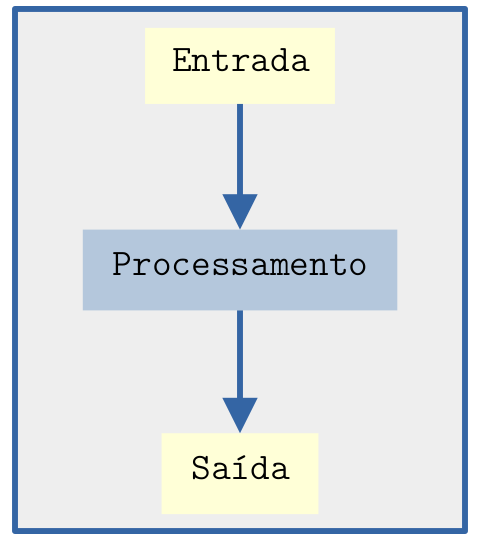
\includegraphics[width=1.5in]{./cap_progest/dados/fig_fg_bloco/fig.png}
  \caption{Bloco de processamento.}
  \label{cap_progest:fig:fg_bloco}
\end{figure}

Blocos podem ser colocados em sequência, selecionados com base em condições lógicas, iterados ou colocados dentro de outros blocos (sub-blocos).

\section{Estruturas de um Programa}\label{cap_progest_sec_est}

\hl{Para escrever qualquer programa, apenas três estruturas são necessárias: \emph{sequência}, \emph{seleção/ramificação} e \emph{iteração}}.

\subsection{Sequência}

A estrutura de \hl{\emph{sequência}} apenas significa que \hl{os blocos de programação são executados em sequência}. Ou seja, a execução de um bloco começa somente após a finalização do bloco anterior.

\begin{figure}[H]
  \centering
  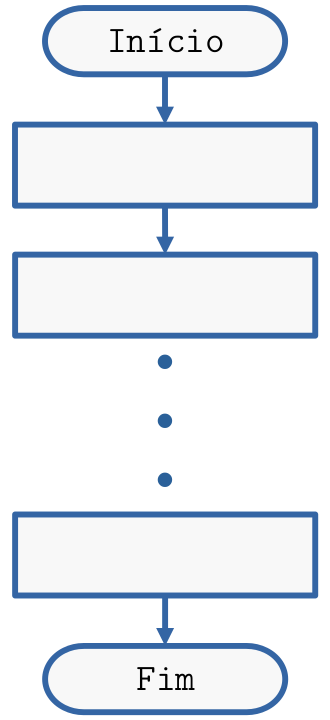
\includegraphics[width=2in]{./cap_progest/dados/fig_fg_sequencia/fig.png}
  \caption{Estrutura de sequência de blocos.}
  \label{cap_progest:fig:fg_sequencia}
\end{figure}

\begin{ex}
  O seguinte código computada a área do triângulo de base e altura informadas pela(o) usuária(o).

\begin{lstlisting}
#início

# bloco: entrada de dados
base = float(input('Digite a base:\n'))
altura = float(input('Digite a altura\n'))

# bloco: computação da área
area = base*altura/2

# bloco: saída de dados
print(f'Área = {area}')

#fim
\end{lstlisting}

O código acima está estruturado em três blocos. O primeiro bloco (linhas 3-5) processa a entrada de dados, seu término ocorre somente após a(o) usuária(o) digitar os valores da base e da altura. Na sequência, o bloco (linhas 7-8) faz a computação da área do triângulo e aloca o resultado na variável \lstinline+area+. No que este bloco termina seu processamento, é executado o último bloco (linhas 10-11), que imprime o resultado na tela.
\end{ex}

\subsection{Ramificação}

\hl{Estruturas de ramificação permitem a seleção de um ou mais blocos com base em condições lógicas}.

\begin{ex}\label{cap_progest_sec_est:ex:ramifica}
  O seguinte código lê um número inteiro digitado pela(o) usuária(o) e imprime uma mensagem no caso do número digitado ser par.

\begin{lstlisting}
#início

# entrada de dados
n = int(input('Digite um número inteiro:\n'))

# ramificação
if n%2 == 0:
  print(f'{n} é par.')

#término
\end{lstlisting}

Observamos que, no caso do número digitado não ser par, o programa termina sem nenhuma mensagem ser impressa. Esse é um exemplo de um bloco de ramificação, a instrução de ramificação (linha 7) testa a condição de \lstinline+n+ ser par. Somente no caso de ser verdadeiro, a instrução de impressão (linha 8) é executada. Após e impressão o programa é encerrado. No caso de \lstinline+n+ não ser par, o programa é encerrado sem que a instrução da linha 8 seja executada, i.e. a mensagem não é impressa.

\begin{figure}[H]
  \centering
  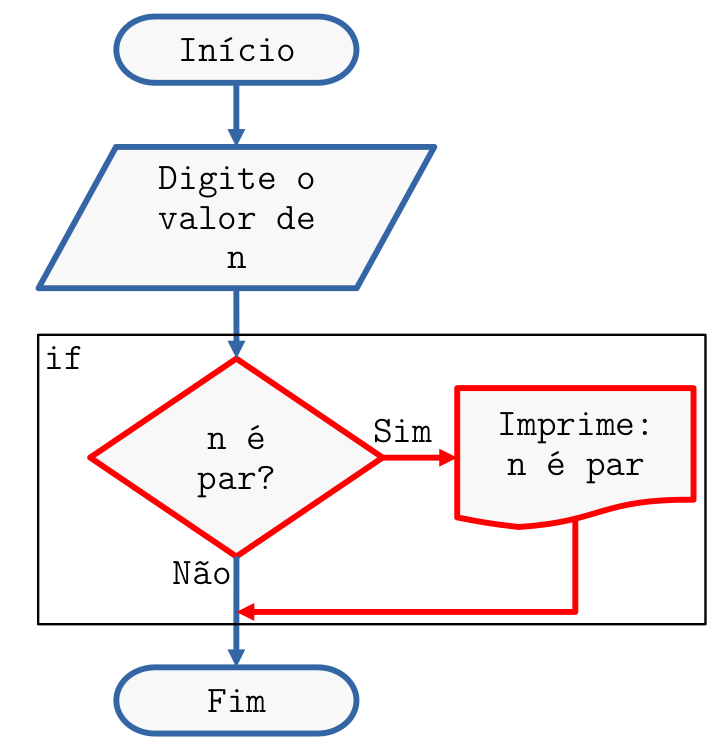
\includegraphics[width=2in]{./cap_progest/dados/fig_fg_ramifica/fig.png}
  \caption{Fluxograma de uma estrutura de ramificação.}
  \label{cap_progest:fig:fg_ramifica}
\end{figure}
  
\end{ex}

\begin{obs}[\hl{Indentação}]
  Na linguagem {\python}, a \emph{indentação} do código marca o início e o fim do bloco de código que pertence à instrução de ramificação. No Exemplo~\ref{cap_progest_sec_est:ex:ramifica}, o bloco selecionado pela instrução {\PYTHONif} é apenas a linha de código 8.
\end{obs}

\subsection{Repetição}

\hl{Instruções de repetição permitem que um mesmo bloco seja processado várias vezes em sequência}. Em {\python}, há duas instruções de repetição disponíveis: {\PYTHONfor} e {\PYTHONwhile}. 

\subsubsection{\texttt{for}}

A instrução \hl{{\PYTHONfor} permite que um bloco seja iterado para cada elemento de uma dada coleção de dados}.

\begin{ex}\label{cap_progest_sec_est:ex:for}
  O seguinte código testa a paridade de cada um dos elementos do conjunto $\{-3, -2, -1, 0, 1, 2, 3\}$.

\begin{lstlisting}
#início

# repetição for
for n in {-3, -2, -1, 0, 1, 2, 3}:
  res = (n%2 == 0)
  print(f'{n} é par? ', res)
    
#término
\end{lstlisting}

A instrução de repetição {\PYTHONfor} (linha 4), aloca em \lstinline+n+ um dos elementos do conjunto. Então, executa em sequência o bloco de comandos das linhas 5 e 6. De forma iterada, \lstinline+n+ recebe um novo elemento do conjunto e o bloco das linhas 5 e 6 é novamente executado. A repetição termina quando todos os elementos do conjunto já tiverem sido iterados. O código segue, então, para a linha 7. Não havendo mais instruções, o programa é encerrado.

\begin{figure}[H]
  \centering
  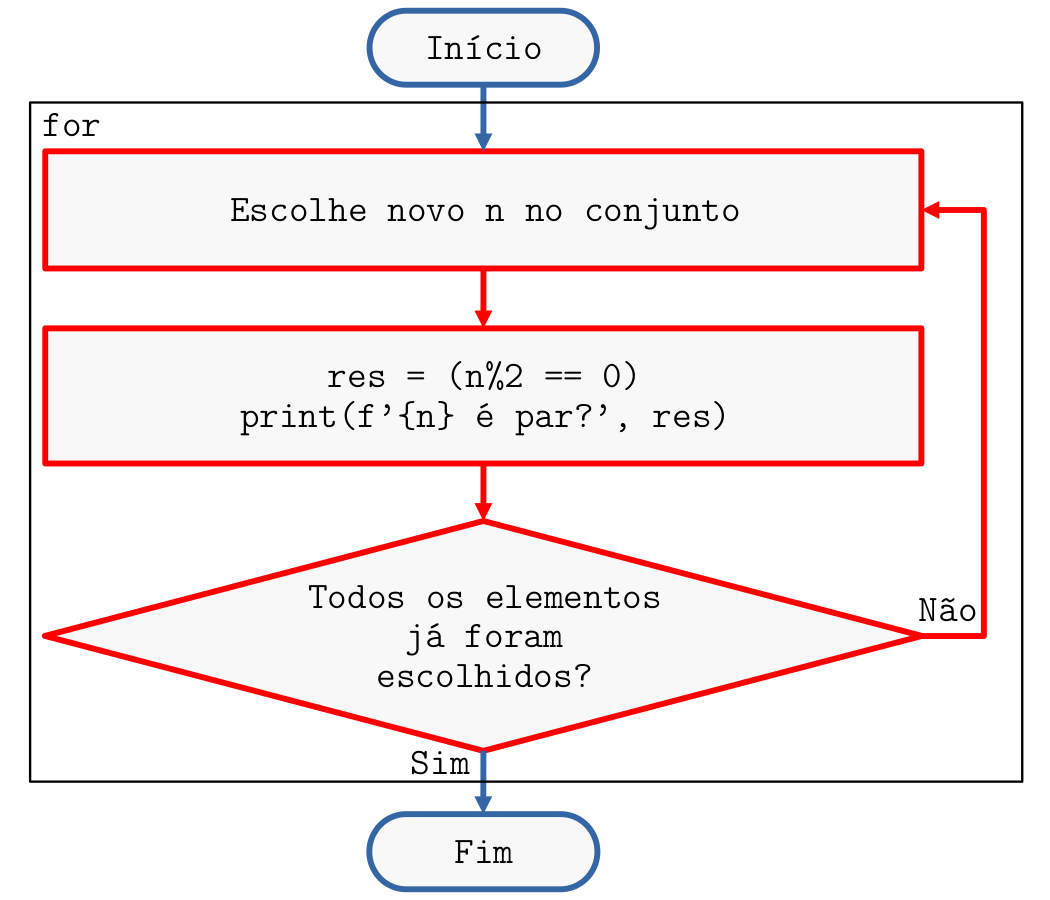
\includegraphics[width=2.75in]{./cap_progest/dados/fig_fg_for/fig.png}
  \caption{Fluxograma de uma estrutura de repetição do tipo {\PYTHONfor}.}
  \label{cap_progest_sec_est:fig:fg_for}
\end{figure}

Assim como no caso de uma instrução de ramificação, \hl{o bloco do {\PYTHONfor} é definido pela indentação do código}. Neste exemplo, o bloco são as linhas 5 e 6.
\end{ex}

\subsubsection{\texttt{while}}

A instrução \hl{{\PYTHONwhile} permite a repetição de um bloco enquanto uma dada condição lógica é satisfeita}.

\begin{ex}\label{cap_progest_sec_est:ex:while}
  O seguinte código testa a paridade dos números inteiros compreendidos de $-3$ a $3$.

\begin{lstlisting}
#início

n = -3

# repetição: while
while n <= 3:
  res = (n%2 == 0)
  print(f'{n} é par?', res)
  n += 1
    
#término
\end{lstlisting}

\begin{figure}[ht]
  \centering
  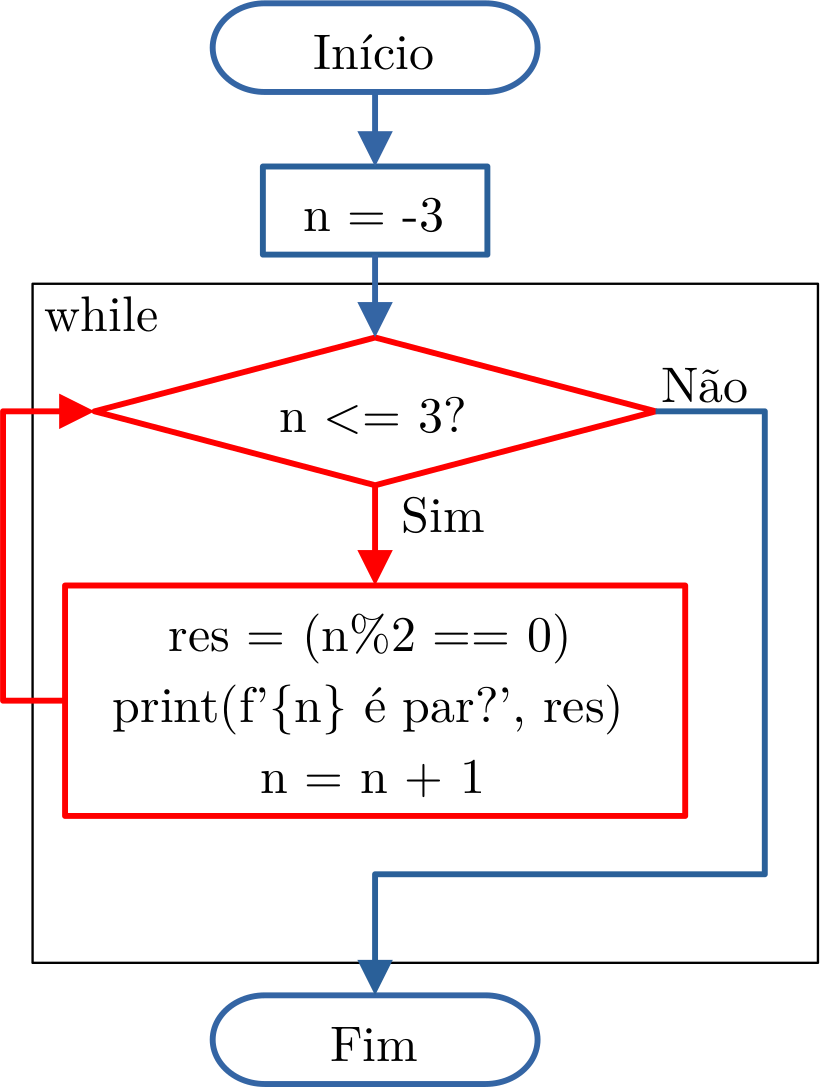
\includegraphics[width=2.5in]{./cap_progest/dados/fig_fg_while_ex/fig.png}
  \caption{Fluxograma da estrutura de repetição do tipo {\PYTHONwhile} para o Exemplo \ref{cap_progest_sec_est:ex:while}.}
  \label{cap_progest_sec_est:fig:fg_while_ex}
\end{figure}


A instrução de repetição {\PYTHONwhile} faz com que o bloco de processamento definido pelas linhas 7-9 seja executado de forma sequencial enquanto o valor de \texttt{n} for menor ou igual a 3. No caso dessa condição ser verdadeira, o bloco (linhas 7-9) é executado e, então a condição é novamente verificada. No caso da condição ser falsa, esse bloco não é executado e o código segue para a linha 10. Não havendo mais nenhuma instrução, o programa é encerrado.

Observamos que, neste exemplo, \hl{o bloco {\PYTHONwhile}} são as linhas 7-9, \hl{determinado pela indentação do código}.
\end{ex}

\subsection{Exercícios}

% exercícios de compreensão

\begin{exer}
  Complete as lacunas.
  \begin{enumerate}[a)]
    \item As seguintes estruturas são suficientes para escrever qualquer programa: \underline{\phantom{sequência}}, \underline{\phantom{seleção}} e \underline{\phantom{iteração}}.
    \item A estrutura de sequência significa que a execução de um bloco começa somente após a \underline{\phantom{finalização}} do bloco anterior.
    \item A estrutura de seleção permite a escolha de execução de um ou mais blocos com base em \underline{\phantom{condições lógicas}}.
    \item O bloco de código de uma instrução de repetição é determinado pela \underline{\phantom{indentação}} do código.
    \item Instruções de \underline{\phantom{repetição}} permitem que um mesmo bloco seja processado várias vezes de forma iterativa.
  \end{enumerate}
\end{exer}
\begin{resp}
  a) sequência, seleção e iteração. b) finalização. c) condições lógicas. d) indentação. e) repetição.
\end{resp}

\begin{exer}
  Complete as lacunas.
  \begin{enumerate}[a)]
    \item Uma estrutura de ramificação é implementada com a instrução \underline{\phantom{\texttt{if}}}.
    \item A instrução \underline{\phantom{\texttt{for}}} permite que um bloco seja iterado para cada elemento de uma coleção de dados iterável.
    \item A instrução \underline{\phantom{\texttt{while}}} permite a repetição de um bloco enquanto uma dada condição lógica é satisfeita.
  \end{enumerate}
\end{exer}
\begin{resp}
  a) \texttt{if}. b) \texttt{for}. c) \texttt{while}.
\end{resp}

% exercícios de programação

\begin{exer}
  Seja a reta de equação
  \begin{equation}
    y = ax + b.
  \end{equation}
  Assumindo $a=2$ e $b=-3$, o seguinte código foi desenvolvido para computar o ponto $x$ de interseção da desta reta com o eixo das abscissas.

\begin{lstlisting}
x = -b/2*a
a = 2
b = -3
print(x)
\end{lstlisting}

Identifique e explique os erros desse código. Então, apresente uma versão corrigida.
\end{exer}
\begin{resp}

\begin{lstlisting}
a = 2
b = -3
x = -b/a
print(x)
\end{lstlisting}

\end{resp}

\begin{exer}\label{cap_progest_sec_est:exer:ramifica_reta}
  Seja a reta de equação
  \begin{equation}
    y = ax + b.
  \end{equation}
  Faça um fluxograma de um programa em que a(o) usuária(o) entra com os valores de $a$ e $b$. No caso de $a\neq 0$, o programa computa e imprime o ponto $x$ da interseção dessa reta com o eixo das abscissas.
\end{exer}
\begin{resp}

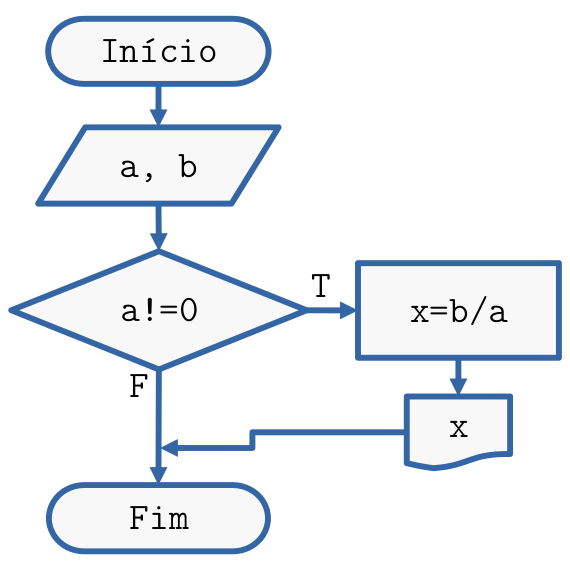
\includegraphics[width=1.5in]{cap_progest/dados/fig_exer_ramifica_reta/fig.png}
  
\end{resp}

\begin{exer}
  Implemente o código referente ao fluxograma criado no Exercício~\exerref{cap_progest_sec_est:exer:ramifica_reta}.
\end{exer}
\begin{resp}

\begin{lstlisting}
a = float(input('Digite o valor de a:\n'))
b = float(input('Digite o valor de b:\n'))
if (a != 0):
  x = -b/(2*a)
  print(f'Ponto de interseção com o eixo x = {x}')
\end{lstlisting}

\end{resp}

\begin{exer}\label{cap_progest_sec_est:exer:for}
  Faça o fluxograma de um programa que usa de um bloco de repetição {\PYTHONfor} para percorrer o conjunto
  \begin{equation}
    A = \{-4, -3, -2, -1, 0, 1, 2, 3, 4\}.
  \end{equation}
  A cada iteração, o programa imprime {\PYTHONTrue} ou {\PYTHONFalse} conforme o elemento seja ímpar ou não.
\end{exer}
\begin{resp}
  
  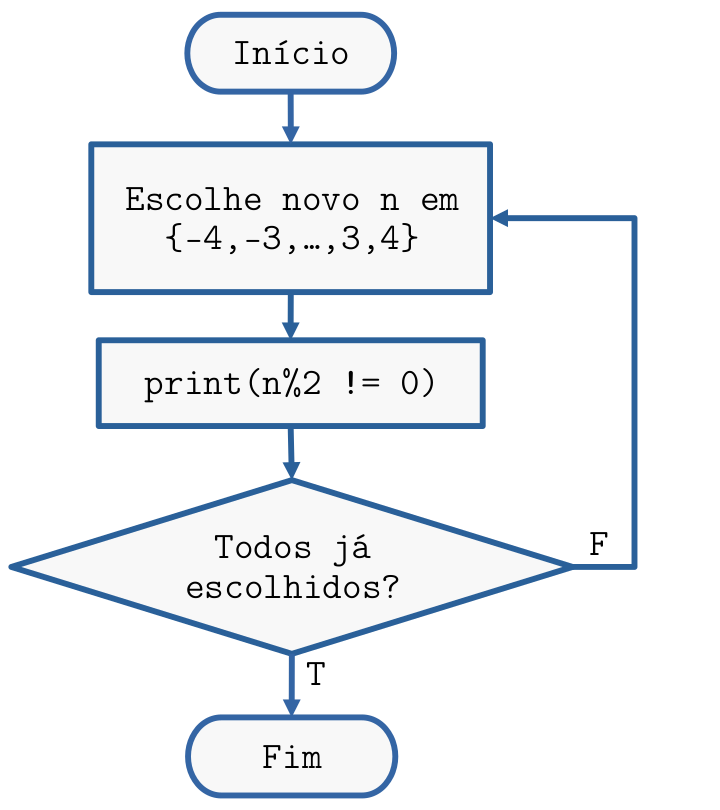
\includegraphics[width=3in]{cap_progest/dados/fig_exer_for/fig.png}

\end{resp}

\begin{exer}
  Implemente o código referente ao fluxograma criado no Exercício~\exerref{cap_progest_sec_est:exer:for}.
\end{exer}
\begin{resp}

\begin{lstlisting}
A = {-4, -3, -2, -1, \
     0, 1, 2, 3, 4}
for x in A:
  res = (x % 2 != 0)
  print(f'{x} é ímpar? {res}')
\end{lstlisting}

\end{resp}

\begin{exer}\label{cap_progest_sec_est:exer:while}
  Faça um fluxograma análogo ao do Exercício~\exerref{cap_progest_sec_est:exer:for} que use a instrução de repetição {\PYTHONwhile} no lugar de {\PYTHONfor}.
\end{exer}
\begin{resp}

  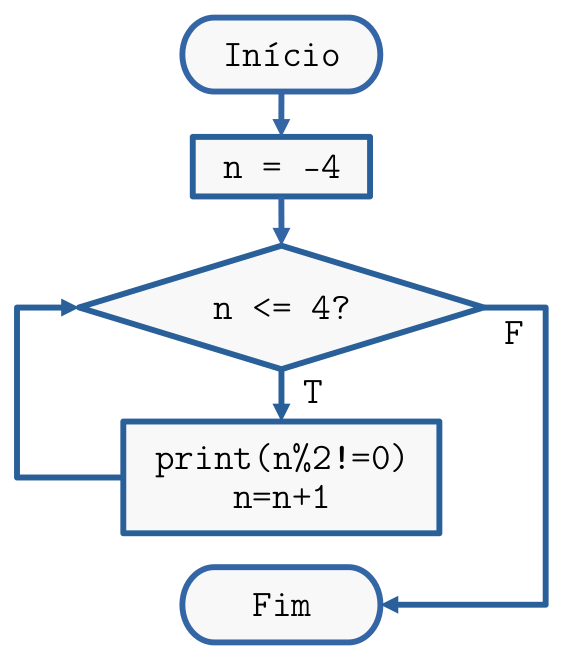
\includegraphics[width=2in]{cap_progest/dados/fig_exer_while/fig.png}

\end{resp}

\begin{exer}
  Implemente um código referente ao fluxograma criado no Exercício~\exerref{cap_progest_sec_est:exer:while}.
\end{exer}
\begin{resp}

\begin{lstlisting}
A = {-4, -3, -2, -1, \
     0, 1, 2, 3, 4}
n = -4
while (n <= 4):
  res = (n % 2 != 0)
  print(f'{n} é ímpar? {res}')
  n += 1
\end{lstlisting}

\end{resp}

\ifisbook
\subsubsection{Respostas}
\shipoutAnswer
\fi


\section{Instruções de Ramificação}\label{cap_progest_sec_ramifica}

\hl{Instruções de ramificação permitem a seleção de blocos de programação com base em condições lógicas}.

\subsection{Instrução \texttt{if}}

\hl{A instrução de ramificação {\PYTHONif} permite a seleção de um bloco de programação com base em uma condição lógica}.

\begin{figure}[H]
  \centering
  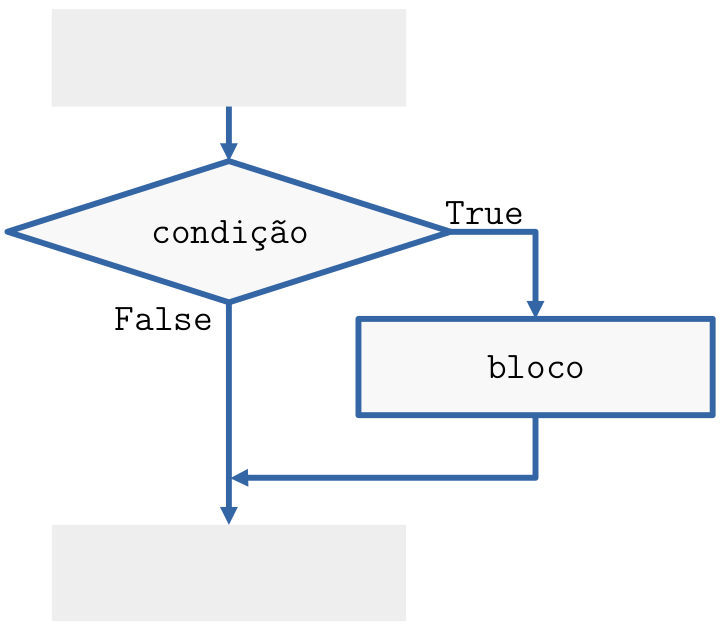
\includegraphics[width=2.25in]{./cap_progest/dados/fig_fg_if/fig.png}
  \caption{Fluxograma de uma ramificação {\PYTHONif}.}
  \label{cap_progest_sec_ramifica:fig:fg_if}
\end{figure}

Em {\python}, a \hl{instrução {\PYTHONif}} tem a seguinte \hl{sintaxe}:

\begin{lstlisting}
bloco_anterior
if condição:
  bloco_0
bloco_posterior
\end{lstlisting}

Se a {\lstinline+condição+} é verdadeira ({\PYTHONTrue}), o bloco (linha 3) é executado. Caso contrário, este bloco não é executado e o fluxo de processamento salta da linha 2 para a linha 6. O bloco selecionado pela instrução {\PYTHONif} é determinado pela indentação do código.

\begin{ex}\label{cap_progest_sec_ramifica:ex:bhaskara_if}
  Seja o polinômio de segundo grau
  \begin{equation}
    p(x) = ax^2 + bx + c.
  \end{equation}
  No caso de existirem, o seguinte código computa as raízes distintas de $p(x)$ para os coeficientes informados pela(o) usuária(o).

\begin{lstlisting}
# entrada de dados
a = float(input('Digite o valor de a:\n'))
b = float(input('Digite o valor de b:\n'))
c = float(input('Digite o valor de c:\n'))

# discriminante
delta = b**2 - 4*a*c

# raízes
if delta > 0:
  # raízes distintas
  x1 = (-b - delta**0.5)/(2*a)
  x2 = (-b + delta**0.5)/(2*a)
  print(f'x_1 = {x1}')
  print(f'x_2 = {x2}')
\end{lstlisting}

\end{ex}

\subsubsection{Escopo de Variáveis}

O \hlemph{escopo} de uma variável é a região em que ela permanece alocada. \hl{O escopo de variáveis alocadas fora do bloco {\PYTHONif} inclui este bloco, mas variáveis alocadas no bloco {\PYTHONif} não permanecem alocadas fora deste}.

\begin{ex}
  No Exemplo~\ref{cap_progest_sec_ramifica:ex:bhaskara_if}, o escopo da variável \lstinline+delta+ inicia-se na linha 7 e permanece válido ao longo do resto do programa. Já, o escopo da variável \lstinline+x1+ compreende somente as linhas 12-15 e, análogo para a variável \lstinline+x2+. 
\end{ex}

\subsection{Instrução \texttt{if-else}}

A instrução \hl{\texttt{if-else} permite a escolha de um bloco ou outro, exclusivamente, com base em uma condição lógica}.

\begin{figure}[H]
  \centering
  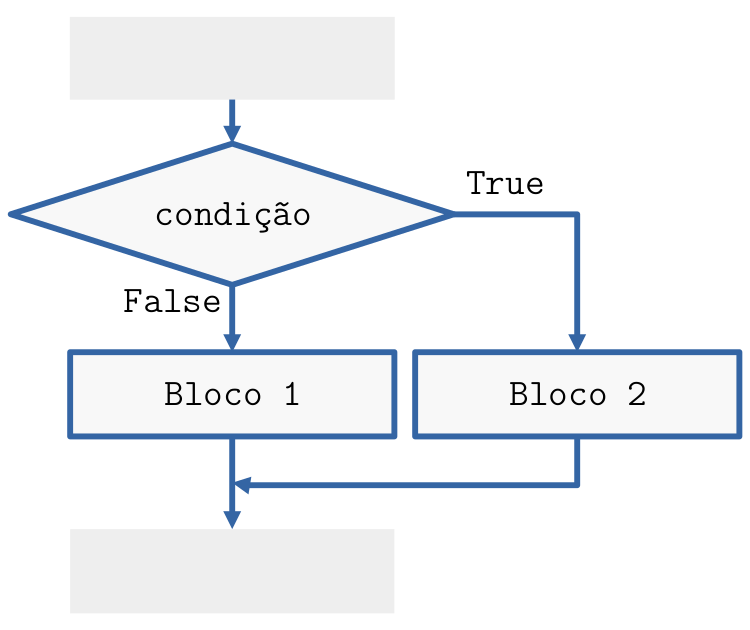
\includegraphics[width=2.25in]{./cap_progest/dados/fig_fg_else/fig.png}
  \caption{Fluxograma de uma ramificação \lstinline+if-else+.}
  \label{cap_progest_sec_ramifica:fig:fg_else}
\end{figure}

Em {\python}, a instrução \lstinline+if-else+ tem a seguinte sintaxe:

\begin{lstlisting}
bloco_anterior
if condição:
  bloco_0
else:
  bloco_1
bloco_posterior
\end{lstlisting}

Se a {\lstinline+condição+} for verdadeira ({\PYTHONTrue}) o {\lstinline+bloco 0+} é executado, senão o {\lstinline+bloco 1+} é executado.

\begin{ex}
  Seja o polinômio de segundo grau
  \begin{equation}
    p(x) = ax^2 + bx + c.
  \end{equation}
  Se existirem, o seguinte código computa as raízes reais do polinômio, senão imprime mensagem informado que elas não são reais.

\begin{lstlisting}
# entrada de dados
a = float(input('Digite o valor de a:\n'))
b = float(input('Digite o valor de b:\n'))
c = float(input('Digite o valor de c:\n'))

# discriminante
delta = b**2 - 4*a*c

# raízes
if delta >= 0:
  x1 = (-b - delta**0.5)/(2*a)
  x2 = (-b + delta**0.5)/(2*a)
  print(f'x_1 = {x1}')
  print(f'x_2 = {x2}')
else:
  print('Não tem raízes reais.')
\end{lstlisting}

\end{ex}

\subsubsection{Instrução \lstinline+if-else+ em Linha}

Por praticidade, {\python} também tem a sintaxe \lstinline+if-else+ em linha:

\begin{lstlisting}
x = valor if True else outro_valor
\end{lstlisting}

\begin{ex}
  O valor absoluto de um número real $x$ é
  \begin{equation}
    |x| := \left\{
      \begin{array}{ll}
        x &, x\geq 0,\\
        -x &, x<0
      \end{array}
    \right.
  \end{equation}
  O seguinte código, computa o valor absoluto\endnote{{\python} tem a função {\PYTHONabs} para computar o valor absoluto de um número.} de um número dado por usuária(o).
  
\begin{lstlisting}
x = float(input('Digite o valor de x:\n'))
abs_x = x if x>=0 else -x
print(f'|x| = {abs_x}')
\end{lstlisting}

\end{ex}

\subsection{Instrução \texttt{if-elif}}

\hl{A instrução \texttt{if-elif} permite a seleção condicional de blocos, sem impor a necessidade da execução de um deles}.

\begin{figure}[H]
  \centering
  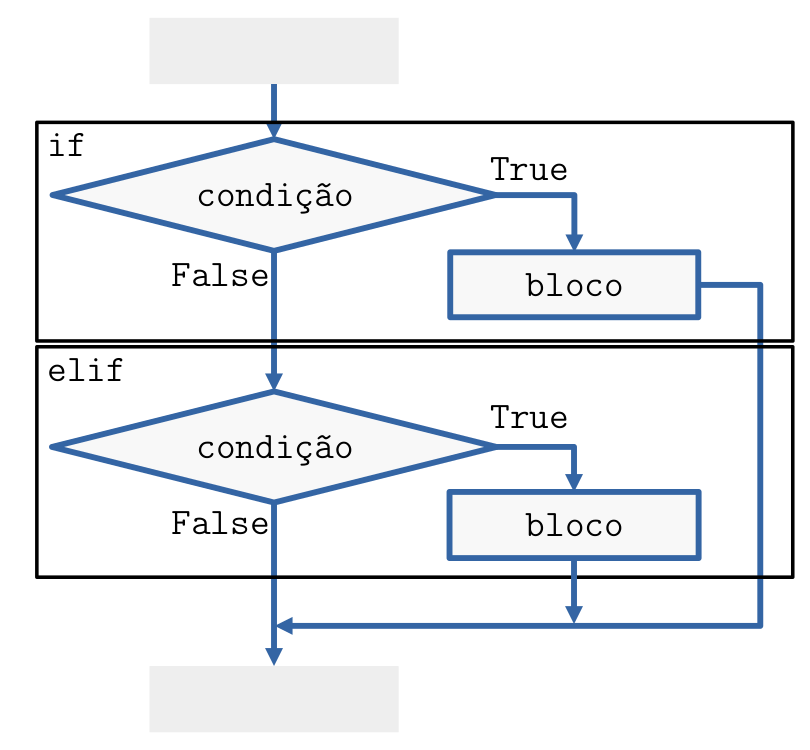
\includegraphics[width=2.5in]{./cap_progest/dados/fig_fg_elif/fig.png}
  \caption{Fluxograma de uma ramificação \lstinline+if-elif+.}
  \label{cap_progest_sec_ramifica:fig:fg_elif}
\end{figure}

Em {\python}, a instrução \lstinline+if-elif+ tem a seguinte sintaxe:

\begin{lstlisting}
bloco_anterior
if condição_0:
  bloco_0
elif condição 1:
  bloco_1
bloco posterior
\end{lstlisting}

Se a \lstinline+condição_0+ for verdadeira ({\PYTHONTrue}), o \lstinline+bloco_0+ é executado. Senão, se a \lstinline+condição_1+ for verdadeira ({\PYTHONTrue}) o \lstinline+bloco_1+ é executado. No caso de ambas as condições serem falsas ({\PYTHONFalse}), os blocos \lstinline+bloco_0+ e \lstinline+bloco_1+ não são executados e o fluxo de processamento segue a partir da linha 6.

\begin{ex}
  Seja o polinômio de segundo grau
  \begin{equation}
    p(x) = ax^2 + bx + c.
  \end{equation}
  Conforme o caso, o seguinte código computa a raiz dupla do polinômio ou suas raízes reais distintas, a partir dos coeficientes informados pela(o) usuária(o).

\begin{lstlisting}
# entrada de dados
a = float(input('Digite o valor de a:\n'))
b = float(input('Digite o valor de b:\n'))
c = float(input('Digite o valor de c:\n'))

# discriminante
delta = b**2 - 4*a*c

# raízes
if delta > 0:
  x1 = (-b - delta**0.5)/(2*a)
  x2 = (-b + delta**0.5)/(2*a)
  print('Raízes reais distintas:')
  print(f'x_1 = {x1}')
  print(f'x_2 = {x2}')
elif delta == 0:
  print('Raiz dupla:')
  x = -b/(2*a)
  print(f'x_1 = x_2 = {x}')
\end{lstlisting}

\end{ex}

\subsection{Instrução \texttt{if-elif-else}}

A instrução \lstinline+if-elif-else+ permite a seleção condicional de blocos, sendo que ao menos um bloco será executado. Em {\python}, sua sintaxe é:

\begin{lstlisting}
bloco_anterior
if condição_0:
  bloco_0
elif condição_1:
  bloco_1
else:
  bloco_2
bloco posterior
\end{lstlisting}

Se a \lstinline+condição_0+ for verdadeira ({\PYTHONTrue}), então o \lstinline+bloco_0+ é executado. Senão, se a \lstinline+condição_1+ for verdadeira ({\PYTHONTrue}), então o \lstinline+bloco_1+ é executado. Senão, o \lstinline+bloco_2+ é executado.

\begin{ex}
  Seja o polinômio de segundo grau
  \begin{equation}
    p(x) = ax^2 + bx + c.
  \end{equation}
  Conforme o caso (raízes reais distintas, raiz dupla ou raízes complexas), o seguinte código computa as raízes desse polinômio, a partir dos coeficientes informados pela(o) usuária(o).

\begin{lstlisting}
# entrada de dados
a = float(input('Digite o valor de a:\n'))
b = float(input('Digite o valor de b:\n'))
c = float(input('Digite o valor de c:\n'))

# discriminante
delta = b**2 - 4*a*c

# raízes
if delta > 0:
  # raízes distintas
  x1 = (-b - delta**0.5)/(2*a)
  x2 = (-b + delta**0.5)/(2*a)
  print('Raízes reais distintas:')
  print(f'x_1 = {x1}')
  print(f'x_2 = {x2}')
elif delta == 0:
  # raiz dupla
  x = -b/(2*a)
  print('Raiz dupla:')
  print(f'x_1 = x_2 = {x}')
else:
  # raízes complexas
  # parte real
  rea = -b/(2*a)
  # parte imaginária
  img = (-delta)**0.5/(2*a)
  x1 = rea - img*1j
  x2 = rea + img*1j
  print('Raízes complexas:')
  print(f'x_1 = {x1}')
  print(f'x_2 = {x2}')
\end{lstlisting}

\end{ex}

\subsection{Múltiplos Casos}

\hl{Pode-se encadear instruções \texttt{if-elif-elif-...-elif[-else]} para a seleção condicional entre múltiplos blocos}.

\begin{ex}
  Sejam as circunferências de equações:
  \begin{align}
    & c_1: (x-a_1)^2 + (y-b_1)^2 = r_1, \\
    & c_2: (x-a_1)^2 + (y-b_1)^2 = r_2.
  \end{align}
  Conforme entradas dadas por usuária(o), o seguinte código informa se um dado ponto $(x, y)$ pertence: à interseção dos discos determinados por $c_1$ e $c_2$, apenas ao disco determinado por $c_1$, apenas ao disco determinado por $c_2$ ou a nenhum desses discos.

\begin{lstlisting}
# entrada de dados
print('c1: (x-a1)**2 + (y-b1)**2 = r1')
a1 = float(input('Digite o valor de a1:\n'))
b1 = float(input('Digite o valor de b1:\n'))
r1 = float(input('Digite o valor de r1:\n'))
print('c2: (x-a2)**2 + (y-b2)**2 = r1')
a2 = float(input('Digite o valor de a2:\n'))
b2 = float(input('Digite o valor de b2:\n'))
r2 = float(input('Digite o valor de r2:\n'))
print('Ponto de interesse (x,y).')
x = float(input('Digite o valor de x:\n'))
y = float(input('Digite o valor de y:\n'))

# pertence ao disco c1?
c1 = (x-a1)**2 + (y-b1)**2 <= r1
# pertence ao disco c2?
c2 = (x-a2)**2 + (y-b2)**2 <= r2

# imprime resultado
if c1 and c2:
  print(f'({x}, {y}) pertence à interseção dos discos.')
elif c1:
  print(f'({x},{y}) pertence ao disco c1.')
elif c2:
  print(f'({x},{y}) pertence ao disco c2.')
else:
  print(f'({x},{y}) não pertence aos discos.')
\end{lstlisting}

\end{ex}


\subsection{Exercícios}

% exercícios de comprensão

\begin{exer}
  Complete as lacunas.
  \begin{enumerate}[a)]
    % a)
    \item Instruções de ramificação permitem a \underline{\phantom{seleção}} de blocos códigos com base em condições lógicas.
    % b)
    \item Uma instrução \underline{\phantom{{\PYTHONif}}} permite a seleção de um bloco de código com base em uma condição \underline{\phantom{lógica}}.
    % c)
    \item O \underline{\phantom{escopo}} de uma variável é a região em que ela permanece alocada.
    % d)
    \item Uma instrução \underline{\phantom{\texttt{else}}} indica a seleção de um bloco de código com base na negação da condição de seleção do bloco imediatamente anterior.
    % e)
    \item Uma instrução \texttt{elif} permite impor uma \underline{\phantom{condição lógica}} adicional para a seleção de um bloco de código com base na negação da condição de seleção do bloco imediatamente anterior.
  \end{enumerate}
\end{exer}
\begin{resp}
  a) seleção; b) lógica; c) escopo; d) \texttt{else}; e) condição lógica
\end{resp}

% exercícios de programação

\begin{exer}
  Seja a equação de reta
  \begin{equation}
    ax + b = 0.
  \end{equation}
  Dados coeficientes $a \neq 0$ e $b$ informados por usuária(o), crie um código que imprime o ponto de interseção dessa reta com o eixo das abscissas. O código não deve tentar computar o ponto no caso de $a=0$. 
\end{exer}
\begin{resp}

\begin{lstlisting}
# entrada de dados
a = float(input('Digite o valor de a:\n'))
b = float(input('Digite o valor de b:\n'))

# computação
if a != 0:
  x = -b/a
  y = a*x + b
  print(f'Intercepta eixo-x em: ({x}, {y}).')
\end{lstlisting}

\end{resp}

\begin{exer}
  Considere o seguinte código.

\begin{lstlisting}
n = int(input('Digite um número inteiro:\n')
if n % 2 == 0:
  m = 1
n = n + m
print(n)
\end{lstlisting}

A ideia é que, se $n$ for ímpar, o código imprime $n$, caso contrário, imprime $n+1$. Este código contém erro. Identifique e explique-o, então proponha uma versão funcional.
\end{exer}
\begin{resp}

\begin{lstlisting}
n = int(input('Digite um número inteiro:\n')
m = 0
if n % 2 == 0:
  m = 1
n = n + m
print(n)
\end{lstlisting}

\end{resp}

\begin{exer}
  Considere o seguinte algoritmo/pseudocódigo para verificar se um dado número inteiro $n$ é par ou ímpar.

\ifisbook
\newpage
\fi
\begin{itemize}\setlength\itemsep{0em}
\item[0.] Início.
\item[1.] Usuária(o) informa o valor inteiro $n$.
\item[2.] Se o resto da divisão de $n$ por $2$ for igual a zero, então faça:
  \begin{itemize}\setlength\itemsep{0em}
  \item[2.1.] Imprime a mensagem: ``$n$ é par.''.
  \end{itemize}
\item[3.] Senão, faça:
  \begin{itemize}\setlength\itemsep{0em}
  \item[3.1] Imprime a mensagem: ``$n$ é ímpar''. 
  \end{itemize}
\item[4.] Fim.
\end{itemize}
Faça um fluxograma para esse algoritmo e implemente-o.
\end{exer}

\begin{exer}
  Considere a equação da circunferência
  \begin{equation}
    c: (x-a)^2 + (y-b)^2 = r^2.
  \end{equation}
  Com dados informados por usuária(o), desenvolva um código que informe se um dado ponto $(x, y)$ pertence ou não ao disco determinado por $c$.
\end{exer}
\begin{resp}

\begin{lstlisting}
# entrada de dados
print('Circunferência c:')
a = float(input('Digite o valor de a:\n'))
b = float(input('Digite o valor de b:\n'))
r = float(input('Digite o valor de r:\n'))
print('Ponto (x, y):')
x = float(input('Digite o valor de x:\n'))
y = float(input('Digite o valor de y:\n'))

# resultado
if (x-a)**2 + (y-b)**2 <= r**2:
  print(f'({x}, {y}) pertence ao disco.')
else:
  print(f'({x}, {y}) não pertence ao disco.')
\end{lstlisting}

\end{resp}

\begin{exer}\label{cap_progest_sec_ramifica:exer:intercep_retas}
  Sejam informadas por usuária(o) os coeficientes das retas
  \begin{align}
    & r_1: a_1x + b_1 = 0, \\
    & r_2: a_2x + b_2 = 0.
  \end{align}
  Crie um código que informe se as retas são paralelas. Caso contrário, o código imprime o ponto de interseção delas.
\end{exer}
\begin{resp}

\begin{lstlisting}
# entrada de dados
print('r1: a1*x + b1 = 0')
a1 = float(input('Digite o valor de a1:\n'))
b1 = float(input('Digite o valor de b1:\n'))
print('r2: a2*x + b2 = 0')
a2 = float(input('Digite o valor de a2:\n'))
b2 = float(input('Digite o valor de b2:\n'))

# resultado
if a1 == a2:
  print('r1 // r2')
else:
  x = (b1-b2)/(a2-a1)
  y = a1*x + b1
  print('Ponto de interseção: ({x}, {y}).')
\end{lstlisting}

\end{resp}

\begin{exer}
  Refaça o código do Exercício~\exerref{cap_progest_sec_ramifica:exer:intercep_retas} de forma a incluir o caso em que as retas sejam coincidentes. Ou seja, o código deve informar os seguintes casos: retas paralelas não coincidentes, retas coincidentes ou, caso contrário, ponto de interseção das retas.
\end{exer}
\begin{resp}

\begin{lstlisting}
# entrada de dados
print('r1: a1*x + b1 = 0')
a1 = float(input('Digite o valor de a1:\n'))
b1 = float(input('Digite o valor de b1:\n'))
print('r2: a2*x + b2 = 0')
a2 = float(input('Digite o valor de a2:\n'))
b2 = float(input('Digite o valor de b2:\n'))

# resultado
if a1 == a2:
  if (b1 == b2):
    print('r1 = r2')
  else:
    print('r1 // r2 e r1 != r2')
else:
  x = (b1-b2)/(a2-a1)
  y = a1*x + b1
  print('Ponto de interseção: ({x}, {y}).')
\end{lstlisting}

\end{resp}

\begin{exer}
  Sejam a parábola de equação
  \begin{equation}
    a_1x^2 + a_2x + a_3 = 0
  \end{equation}
  e a reta
  \begin{equation}
    b_1x + b_2 = 0.
  \end{equation}
  Conforme os coeficientes dados por usuária(o), desenvolva um código que imprime o(s) ponto(s) de interseção da reta com a parábola. O código deve avisar os casos em que: há apenas um ponto, há dois pontos ou não há ponto de interseção.
\end{exer}
\begin{resp}

\begin{lstlisting}
# entrada de dados
print('Coeficientes da parábola')
print('a1*x**2 + a2*x + a3 = 0')
a1 = float(input('Digite o valor de a1:\n'))
a2 = float(input('Digite o valor de a2:\n'))
a2 = float(input('Digite o valor de a3:\n'))

print('Coeficientes da reta')
print('b1*x + b2 = 0')
b1 = float(input('Digite o valor de b1:\n'))
b2 = float(input('Digite o valor de b2:\n'))

# discriminante da equação
# a1*x**2 + (a2-b1)*x + (a3-b2) = 0
delta = (a2-b1)**2 - 4*a1*(a3-b2)

# ponto(s) de interseção
if delta == 0:
  x = (b1-a2)/(2*a1)
  y = b1*x + b2
  print('Ponto de interseção:')
  print(f'({x}, {y})')
elif delta > 0:
  x1 = ((b1-a2) - delta**2)/(2*a1)
  y1 = b1*x1 + b2
  x2 = ((b1-a2) + delta**2)/(2*a1)
  y2 = b1*x2 + b2
  print('Pontos de interseção:')
  print(f'({x1}, {y1}), ({x2}, {y2})')
else:
  print('Não há ponto de interseção.')
\end{lstlisting}

\end{resp}

\begin{exer}
  Com dados informados por usuária(o), sejam as circunferências de equações
  \begin{align}
    & c_1: (x-a_1)^2 + (y-b_1)^2 = r_1^2, \\
    & c_2: (x-a_2)^2 + (y-b_2)^2 = r_2^2.
  \end{align}
  Desenvolva um código que informe a(o) usuária(o) dos seguintes casos: $c_1$ e $c_2$ são coincidentes, $c_1\cap c_2$ tem dois pontos, $c_1\cap c_2$ tem somente um ponto, $c_1\cap c_2 = \emptyset$.
\end{exer}
\begin{resp}

\begin{lstlisting}
# entrada de dados
print('c1: (x-a1)**2 + (y-b1)**2 = r1**2')
a1 = float(input('Digite o valor de a1:\n'))
b1 = float(input('Digite o valor de b1:\n'))
r1 = float(input('Digite o valor de r1:\n'))
print('c2: (x-a2)**2 + (y-b2)**2 = r2**2')
a2 = float(input('Digite o valor de a2:\n'))
b2 = float(input('Digite o valor de b2:\n'))
r2 = float(input('Digite o valor de r2:\n'))

# verificações
if a1==a2 and b1==b2 and r1==r2:
  print('c1 = c2')
else:
  # distância entre os centros
  dist = ((a2-a1)**2 + (b2-b1)**2)**0.5
  if (abs(dist - (r1+r2)) < 1e-15):
    print('c1 & c2 têm um único ponto de interseção.')
  elif (dist < r1+r2):
    print('c1 & c2 têm dois pontos de interseção.')
  else:
    print('c1 & c2 não tem ponto de interseção.')
\end{lstlisting}

\end{resp}

\begin{exer}
  Crie uma calculadora simples. A(o) usuária(o) entra com dois números decimais \lstinline+x+ e \lstinline+y+ e uma das seguintes operações: \lstinline!+!, \lstinline+-+, \lstinline+*+ ou \lstinline+/+. Então, o código imprime o resultado da operação.
\end{exer}
\begin{resp}

\begin{lstlisting}
# entrada de dados
x = float(input('Digite o valor de x:\n'))
op = input('Digite uma das operações +, -, * ou /:\n')
y = float(input('Digite o valor de y:\n'))

# calcula
if op == '+':
  print(f'{x} ' + op + f' {y} = {x+y}')
elif op == '-':
  print(f'{x} ' + op + f' {y} = {x-y}')
elif op == '*':
  print(f'{x} ' + op + f' {y} = {x*y}')
elif op == '/':
  print(f'{x} ' + op + f' {y} = {x/y}')
else:
  print('Desculpa, não entendi!')
\end{lstlisting}

\end{resp}

\begin{exer}\label{cap_progest_sec_ramifica:exer:entre_curvas}
  Informado um ponto $P = (x, y)$ por usuária(o), desenvolva um código que verifique se $P$ está entre as curvas $x = -1$, $x = 2$, $y = x^2$ e $y = x+2$. Consulte a figura abaixo.
\begin{figure}[H]
  \centering
  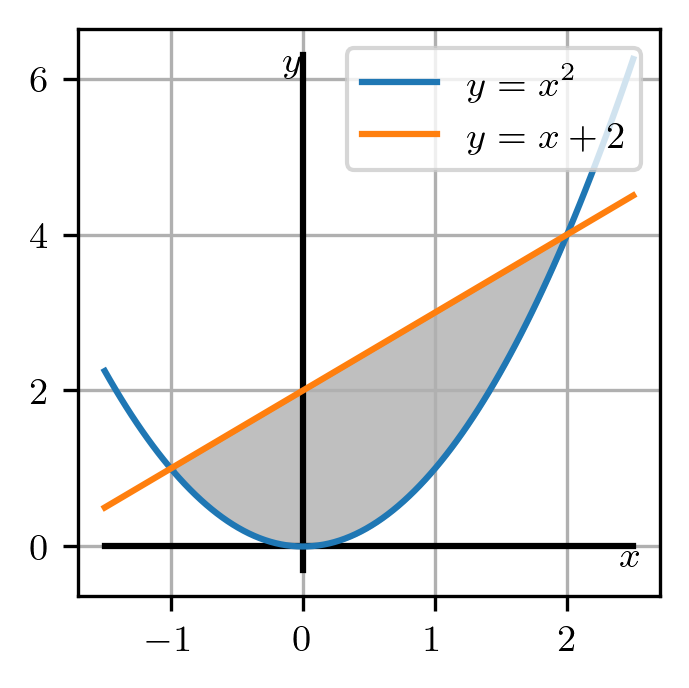
\includegraphics[width=3.75in]{./cap_progest/dados/fig_exer_entre_curvas/fig.png}
\end{figure}
\end{exer}
\begin{resp}

\begin{lstlisting}
print('P = (x,y)')
x = float(input('Digite o valor de x: '))
y = float(input('Digite o valor de y: '))

if x >= -1. and x <= 2 \
   and y >= x**2 and y <= x+2:
  print(f'P = ({x}, {y}) está entre as curvas.')
else:
  print(f'P = ({x}, {y}) não está entre as curvas.')
\end{lstlisting}

\end{resp}

\begin{exer}
  Considere um polinômio da forma
  \begin{equation}
    p(x) = (x-a)(bx^2 + cx + d).
  \end{equation}
  Desenvolva um código para a computação das raízes de $p(x)$, sendo os coeficientes $a$, $b$, $c$ e $d$ (números decimais) informados por usuária(o).
\end{exer}
\begin{resp}

\begin{lstlisting}
print('p(x) = (x-a)(bx^2 + cx + d)')
# entrada de dados
a = float(input('Digite o valor de a: '))
b = float(input('Digite o valor de b: '))
c = float(input('Digite o valor de c: '))
d = float(input('Digite o valor de d: '))

# cálculo das raízes
x1 = a
print(f'x1 = {x1}')
if b != 0.:
  delta = c**2 - 4*b*d
  x2 = (-c - delta**0.5)/(2*b)
  x3 = (-c + delta**0.5)/(2*b)
  print(f'x2 = {x2}')
  print(f'x3 = {x3}')
elif c != 0.:
  x2 = -d/c
  print(f'x2 = {x2}')
\end{lstlisting}

\end{resp}

\ifisbook
\newpage
\subsubsection{Respostas}
\shipoutAnswer
\fi


\section{Instruções de Repetição}\label{cap_progest_sec_repete}

\hl{Estruturas de repetição permitem a execução de um bloco de código várias vezes}. O número de vezes que o bloco é repetido pode depender de uma condição lógica (instrução {\PYTHONwhile}) ou do número de itens de um objeto iterável (instrução{\PYTHONfor}).

\subsection{Instrução \texttt{while}}

\hl{A instrução {\PYTHONwhile} permite a repetição condicional de um bloco de código}. Em {\python}, sua sintaxe é

\begin{lstlisting}
bloco_anterior
while condição:
  bloco
bloco_posterior
\end{lstlisting}

\begin{figure}[H]
  \centering
  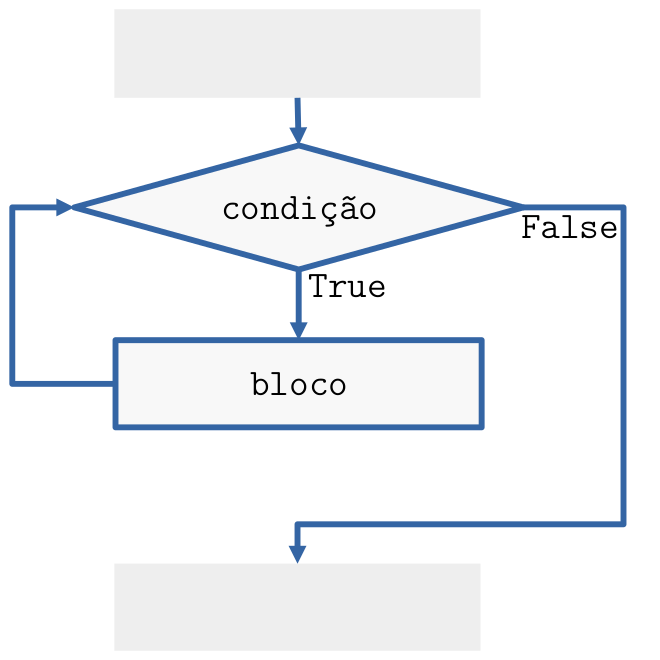
\includegraphics[width=2in]{./cap_progest/dados/fig_fg_while/fig.png}
  \caption{Fluxograma da estrutura de repetição {\PYTHONwhile}.}
  \label{fig:cap_progest_sec_repete:fig:fg_while}
\end{figure}

\begin{ex}\normalfont{(\hl{Somatório com \texttt{while}})}\label{cap_progest_ec_repete:ex:while_soma_num}
  O seguinte código, computa o \href{https://pt.wikipedia.org/wiki/Somat%C3%B3rio}{somatório}
  \begin{align}
    & s = \sum_{i=1}^{n}i \\
    & \text{}\quad = 1 + 2 + 3 + \cdots + n.
  \end{align}

\begin{lstlisting}
n = int(input('Digite um número natural n:\n'))

soma = 0
i = 1
while i <= n:
  soma = soma + i
  i = i + 1

print(f'1 + ... + {n} = {soma}')
\end{lstlisting}

\end{ex}

\begin{ex}\normalfont{\hl{(Aproximando a $\sqrt{x}$.)}}\label{cap_progest_sec_repete:ex:heron}
  O \href{https://en.wikipedia.org/wiki/Methods_of_computing_square_roots#Heron's_method}{método de Heron}{\heron} é um algoritmo para o cálculo aproximado da raiz quadrada de um dado número $x$, i.e. $\sqrt{x}$. Consiste na iteração\endnote{Aqui, assumimos a aproximação inicial $s^{(0)} = 1$, mas qualquer outro número não negativo pode ser usado.}
  \begin{align}
    & r^{(0)} = 1, \\
    & r^{(k+1)} = \frac{1}{2}\left(r^{(k)} + \frac{x}{r^{(k)}}\right),
  \end{align}
  para $k=0,1,2,\ldots,n-1$, onde $n$ é o número de iterações calculadas. Para $x\geq 0$ fornecido por usuária(o), o seguinte código computa a aproximação $r^{(5)}\approx \sqrt{x}$.

\begin{lstlisting}
x = float(input('Digite um número não negativo para x:\n'))
r = 1
k = 0
print(f'{k}: {r}')
while k < 5:
  r = 0.5*(r + x/r)
  k = k + 1
  print(f'{k}: {r}')
print(f'sqrt({x}) = {r}')
\end{lstlisting}

\end{ex}

\subsubsection{\texttt{break}}

\hl{A instrução {\PYTHONbreak} permite interromper um bloco de repetição e sair dele no momento em que ela é alcançada}.

\begin{ex}\label{cap_progest_sec_repete:ex:heron_break}
  No Exemplo \ref{cap_progest_sec_repete:ex:heron}, podemos observar que as aproximações $s^{(k)}\approx \sqrt{x}$ vão se tornando muito próximas umas das outras conforme as iterações convergem. Dessa observação, faz sentido que interrompamos as computações no momento em que a $k+1$-ésima iterada satisfaça
  \begin{equation}
    \left|r^{(k+1)}-r^{(k)}\right| < \texttt{tol}
  \end{equation}
  para alguma tolerância \lstinline+tol+ desejada.

\begin{lstlisting}
max_iter = 50
tol = 1e-15

x = float(input('Digite um número não negativo para x:\n'))

r0 = 1
k = 0
print(f'{k}: {r}')
while k < max_iter:
  k = k + 1
  r = 0.5*(r0 + x/r0)
  print(f'{k}: {r}')
  if (abs(r-r0) < tol):
    break
  r0 = r
print(f'sqrt({x}) = {r}')
\end{lstlisting}

\end{ex}

\subsection{Instrução \texttt{for}}

\hl{A instrução {\PYTHONfor} iteração de um bloco de código para todos os itens de um dado objeto}. Em {\python}, sua sintaxe é

\begin{lstlisting}
bloco_anterior
for x in Iterável:
  bloco
bloco_posterior
\end{lstlisting}

Pode-se percorrer qualquer objeto iterável ({\PYTHONset}, {\PYTHONtuple}, {\PYTHONlist}, {\PYTHONdict}, etc.). \hl{Em cada iteração, o índice \texttt{x} toma um novo item do objeto. A repetição termina quando todos os itens do objeto tiverem sido escolhidos}. No caso de iteráveis ordenados ({\PYTHONtuple}, {\PYTHONlist}, {\PYTHONdict}, etc.), os itens são iterados na mesma ordem em que estão alocados no objeto.

\begin{ex}\label{cap_progest_sec_repete:ex:media_for}
  O seguinte código, computa a média aritmética do conjunto de números
  \begin{equation}
    A = \{1, 3, 5, 7, 9\}.
  \end{equation}

\begin{lstlisting}
soma = 0
for x in {1,3,5,7,9}:
  soma = soma + x
media = soma/5
print(f'média = {media}')
\end{lstlisting}

\end{ex}

\subsubsection{\texttt{range}}

\hl{A função {\PYTHONrange}([start], stop, [step]), retorna uma sequência iterável de números inteiros}, com início em \lstinline+start+ (padrão \lstinline+start=0+), passo \lstinline+step+ (padrão \lstinline+step=1+) e limite em \lstinline+stop+.

\begin{ex}
  Estudamos os seguinte casos:
  \begin{enumerate}[a)]
  \item Imprime, em ordem crescente, os primeiros $11$ números naturais.

\begin{lstlisting}[xrightmargin=2.5em]
for i in range(11):
  print(i)
\end{lstlisting}

\item Imprime, em ordem crescente, os números naturais contidos de $3$ a $13$, inclusive.

\begin{lstlisting}[xrightmargin=2.5em]
for i in range(3,14):
  print(i)
\end{lstlisting}

\item Imprime, em ordem crescente, os números naturais ímpares contidos de $3$ a $13$, inclusive.

\begin{lstlisting}[xrightmargin=2.5em]
for i in range(3,14,2):
  print(i)
\end{lstlisting}

\item Imprime, em ordem decrescente, os números naturais contidos de $3$ a $13$, inclusive.

\begin{lstlisting}[xrightmargin=2.5em]
for i in range(13,2,-1):
  print(i)
\end{lstlisting}

\end{enumerate}

\end{ex}

\begin{ex}\normalfont{(\hl{Somatório com \texttt{for}}.)}\label{cap_progest_ec_repete:ex:for_soma_num}
  No Exemplo \ref{cap_progest_ec_repete:ex:while_soma_num}, computados
  \begin{equation}
    s = \sum_{i=1}^n i
  \end{equation}
  usando um laço {\PYTHONwhile}. Aqui, apresentamos uma nova versão do código com a instrução {\PYTHONfor}.

\begin{lstlisting}
n = int(input('Digite um número natural n:\n'))
soma = 0
for i in range(1,n+1):
  soma = soma + i
print(f'1 + ... + {n} = {soma}')
\end{lstlisting}

\end{ex}

\begin{ex}
  No Exemplo \ref{cap_progest_sec_repete:ex:heron_break}, apresentamos um código para o cálculo aproximado de $\sqrt{x}$ pelo Método de Heron. Aqui, temos uma nova versão com a instrução {\PYTHONfor} no lugar do laço {\PYTHONwhile}.

\begin{lstlisting}
max_iter = 50
tol = 1e-15

x = float(input('Digite um número não negativo para x:\n'))

r0 = 1
k = 0
print(f'{k}: {r}')
for k in range(max_iter):
  r = 0.5*(r0 + x/r0)
  print(f'{k+1}: {r}')
  if (abs(r-r0) < tol):
    break
  r0 = r
print(f'sqrt({x}) = {r}')
\end{lstlisting}

\end{ex}

\subsection{Exercícios}

% exercícios de compreensão

\begin{exer}
  Complete as lacunas.
  \begin{enumerate}[a)]
    % a)
    \item Intruções de \underline{\phantom{repetição}} permitem a execução de um bloco de código várias vezes.
    % b)
    \item A instrução \underline{\phantom{{\PYTHONwhile}}} permite a repetição de um bloco de código com base em uma condição lógica.
    % c)
    \item A instrução {\PYTHONfor} permite a repetição \underline{\phantom{iterada}} de um bloco de código.
  \end{enumerate}
\end{exer}
\begin{resp}
  a) repetição; b) {\PYTHONwhile}; c) iterada.
\end{resp}

% exercícios de programação

\begin{exer}
  Faça o fluxograma do código apresentado no Exemplo \ref{cap_progest_ec_repete:ex:while_soma_num}. Também, desenvolva uma versão melhorada do código, que verifica se o valor de $n$ digitado pela(o) usuária(o) é não negativa. Caso afirmativo, computa o somatório, noutro caso apenas imprime mensagem de que o $n$ deve ser não negativo.
\end{exer}
\begin{resp}

\begin{lstlisting}
n = int(input('Digite um número natural n:\n'))
if (n >= 0):
  soma = 0
  i = 1
  while (i <= n):
    soma = soma + i
    i = i + 1

  print(f'1 + ... + {n} = {soma}')
else:
  print('ERRO: n deve ser não negativo.')
\end{lstlisting}

\end{resp}

\begin{exer}
  Faça um fluxograma para o código apresentado no Exemplo \ref{cap_progest_sec_repete:ex:media_for}.
\end{exer}
\begin{resp}
  Dica: consulte o fluxograma apresentado no Exemplo \ref{cap_progest_sec_est:ex:for}.
\end{resp}

\begin{exer}
  Crie um objeto do tipo {\PYTHONrange} para cada uma das seguintes sequências:
  \begin{enumerate}
  \item Sequência crescente de todos os números inteiros de $0$ até $99$, inclusive.
  \item Sequência crescente de todos os números pares de $-5$ até $15$.
  \item Sequência decrescente de todos os números de $100$ a $0$, inclusive.
  \item Sequência decrescente de todos os números múltiplos de $3$ entre $17$ e $-3$.
  \end{enumerate}
\end{exer}
\begin{resp}
  \begin{enumerate}[a)]
  \item \lstinline+range(100)+
  \item \lstinline+range(-4,15,2)+
  \item \lstinline+range(100,-1,-1)+
  \item \lstinline+range(15,-4,-3)+
  \end{enumerate}
\end{resp}

\begin{exer}
  Considere o somatório entre dois números inteiros $n \leq m$
  \begin{align}
    & s = \sum_{i=n}^m i \\
    & \text{}\quad = n + (n+1) + (n+2) + \cdots + m
  \end{align}
  Com números informados pela(o) usuária(o), escreva duas versões de códigos para a computação desse somatório:
  \begin{enumerate}[a)]
  \item Usando a instrução {\PYTHONwhile}.
  \item Usando a instrução {\PYTHONfor}.
  \end{enumerate}
\end{exer}
\begin{resp}
a)

\begin{lstlisting}
n = int(input('Digite um número inteiro n:\n'))
m = int(input('Digite um número inteiro m>n:\n'))
soma = 0
i = n
while (i<=m):
  soma = soma + i
  i = i + 1
print(f'n+...+m = {soma}')
\end{lstlisting}

b)

\begin{lstlisting}
n = int(input('Digite um número inteiro n:\n'))
m = int(input('Digite um número inteiro m>n:\n'))
soma = 0
for i in range(n,m+1):
  soma = soma + i
print(f'n+...+m = {soma}')
\end{lstlisting}

\end{resp}

\begin{exer}
  A \href{https://pt.wikipedia.org/wiki/S\%C3\%A9rie_harm\%C3\%B3nica_(matem\%C3\%A1tica)}{série harmônica} é
  \begin{equation}
    \sum_{k=1}^\infty \frac{1}{k} = 1 + \frac{1}{2} + \frac{1}{3} + \cdots + \frac{1}{n} + \cdots
  \end{equation}
  Com $n$ fornecido por usuária(o), crie códigos que computem o valor da soma harmônica
  \begin{equation}
    s = \sum_{k=1}^n \frac{1}{k} = 1 + \frac{1}{2} + \frac{1}{3} + \cdots + \frac{1}{n}.
  \end{equation}
  \begin{enumerate}[a)]
  \item Use uma estrutura de repetição {\PYTHONwhile}.
  \item Use uma estrutura de repetição {\PYTHONfor}.
  \end{enumerate}
\end{exer}
\begin{resp}
a)

\begin{lstlisting}
n = int(input('Digite um número natural n:\n'))
s = 0
k = 1
while (k <= n):
  s = s + 1/k
  k = k + 1
print(s)
\end{lstlisting}

b)

\begin{lstlisting}
n = int(input('Digite um número natural n:\n'))
s = 0
for k in range(n):
  s = s + 1/(k+1)
print(s)
\end{lstlisting}

\end{resp}

\begin{exer}
  O cálculo do logaritmo natural pode ser feito pela seguinte série de potências
  \begin{equation}
    \ln(1 + x) = \sum_{k=1}^\infty (-1)^{k+1}\frac{x^k}{k}
  \end{equation}
  Desenvolva um código que compute a aproximação do $ln(2)$ dada por
  \begin{equation}
    \ln(2) = \sum_{k=1}^n \frac{(-1)^{k+1}}{k}
  \end{equation}
  com $n >= 1$ número inteiro fornecido por usuária(o).
  \begin{enumerate}[a)]
  \item Use uma estrutura de repetição \verb+while+.
  \item Use uma estrutura de repetição \verb+for+.
  \end{enumerate}
\end{exer}
\begin{resp}
  a)

\begin{lstlisting}
n = int(input('Digite um número natural n >= 1: '))

s = 0
k = 1
while (k <= n):
  s += (-1)**(k+1)/k
  k += 1
print(f'ln(2) aprrox. {s}')
\end{lstlisting}

b)

\begin{lstlisting}
n = int(input('Digite um número natural n >= 1: '))

s = 0
for k in range(1, n+1):
  s += (-1)**(k+1)/k
  k += 1
print(f'ln(2) aprrox. {s}')
\end{lstlisting}

\end{resp}

\begin{exer}
  O \href{https://pt.wikipedia.org/wiki/Fatorial}{fatorial} de um número natural é definido pelo \href{https://pt.wikipedia.org/wiki/Produt\%C3\%B3rio}{produtório}
  \begin{align}
    & n! := \prod_{k=1}^{n}k \\
    & \text{}\quad = 1\cdot 2\cdot 3 \cdot (n-1)\cdot n
  \end{align}
  e $0! := 1$. Com $n$ informado por usuária(o), crie códigos para computar $n!$ usando:
  \begin{enumerate}[a)]
  \item uma estrutura de repetição {\PYTHONwhile}.
  \item uma estrutura de repetição {\PYTHONfor}.
  \end{enumerate}
\end{exer}
\begin{resp}
  a)

\begin{lstlisting}
n = int(input('Digite um número natural n:\n'))
fat = 1
k = 1
while (k < n):
  k = k + 1
  fat = fat * k
print(f'{n}! = {fat}')
\end{lstlisting}

b)

\begin{lstlisting}
n = int(input('Digite um número natural n:\n'))
fat = 1
for k in range(1,n+1):
  fat = fat * k
print(f'{n}! = {fat}')
\end{lstlisting}

\end{resp}

\begin{exer}
  O \href{https://pt.wikipedia.org/wiki/E_(constante_matem\%C3\%A1tica)}{número de Euler}{\euler} é tal que
  \begin{align}
    & e := \sum_{k=0}^\infty \frac{1}{n!} \\
    & \text{}\quad = \frac{1}{0!} + \frac{1}{1!} + \frac{1}{2!} + \cdots + \frac{1}{n!} + \cdots
  \end{align}
  Com $n$ fornecido por usuária(o), desenvolva um código que computa a aproximação
  \begin{equation}
    e \approx e^{(n)} = \sum_{k=0}^n \frac{1}{n!}.
  \end{equation}
  Qual o número $n$ tal que $\left|e^{(n)} - e^{(n-1)}\right|<10^{-15}$?
\end{exer}
\begin{resp}

\begin{lstlisting}
n = int(input('Digite um número natural n:\n'))
fat = 1
e = 1
for k in range(1,n+1):
  fat = fat * k
  e = e + 1/fat
print(f'e = {e}')
\end{lstlisting}

\end{resp}

\begin{exer}
  Com $n\geq 1$ número natural fornecido por usuária(o), crie um código que verifique se $n$ é um \href{https://pt.wikipedia.org/wiki/N\%C3\%BAmero_primo}{número primo}.
\end{exer}
\begin{resp}

\begin{lstlisting}
n = int(input('Digite um número natural n>=1:\n'))
primo = True
for i in range(2, n//2+1):
  if (n % i == 0):
    primo = False
    break
print(f'{n} é primo? {primo}')
\end{lstlisting}

\end{resp}

\ifisbook
\subsubsection{Respostas}
\shipoutAnswer
\fi

\chapter{Funções}\label{cap_fun}

Uma \hl{\emph{função} (ou método) é um \emph{subprograma} (ou subalgoritmo)}, um bloco de programação para o processamento de uma tarefa e que pode ser chamado à execução, sempre que necessário, pelo programa a que pertence.

\section{Funções Predefinidas e Módulos}\label{cap_fun_sec_buildin}

\subsection{Funções Predefinidas}

Como o nome indica, \hl{\emph{funções predefinidas} são aquelas disponíveis por padrão na linguagem de programação}, i.e. sem a necessidade de serem explicitamente definidas no código. As \hl{funções predefinidas do {\python}} podem ser consultadas em
\begin{center}
  \url{https://docs.python.org/3/library/functions.html}
\end{center}

Nós já vinhamos utilizando várias dessas funções.

\subsubsection{Entrada e Saída de Dados}

Na entrada e saída de dados, utilizamos
\begin{itemize}
\item {\PYTHONinput} \hlemph{entrada}

  Essa função lê uma linha digitada no \textit{prompt}, converte-a em uma \textit{string} e a retorna. Admite como entrada uma \textit{string} que é impressa no \textit{prompt} antes da leitura.

\item {\PYTHONprint} \hlemph{saída}

  Essa função recebe um objeto e o imprime em formato texto, por padrão, no \textit{prompt} de saída.

\begin{lstlisting}[xrightmargin=2.5em]
>>> s = input('Olá, qual o seu nome? ')
Olá, qual o seu nome? Fulane
>>> print(f'Bem vinde, {s}!')
Bem vinde, Fulane!
\end{lstlisting}

\end{itemize}

\subsubsection{Construtores de Dados}

Temos as funções que constroem objetos de classes de números:
\begin{itemize}

\item \lstinline+bool()+ \hlemph{booleano}

  Recebe um objeto e retorna outro da classe {\PYTHONbool}.

\begin{lstlisting}[xrightmargin=2.5em]
>>> bool(0)
False
>>> bool(1)
True
>>> bool('')
False
>>> bool('0')
True
\end{lstlisting}
  
\item \lstinline+int()+ \hlemph{inteiro}

  Recebe um número ou \textit{string} \lstinline+x+ e retorna um objeto da classe {\PYTHONint}.

\begin{lstlisting}[xrightmargin=2.5em]
>>> int(-2.1)
-2
>>> int(3.9)
3
>>> int(5.5)
5
>>> int('51')
51
\end{lstlisting}

\item \lstinline+float()+ \hlemph{decimal}

  Recebe um número ou \textit{string} \lstinline+x+ e retorna um objeto da classe {\PYTHONfloat}.

\begin{lstlisting}[xrightmargin=2.5em]
>>> float(1)
1.0
>>> float('-2.7')
-2.7
\end{lstlisting}

\item \lstinline+complex()+ \hlemph{complexo}

  Recebe as partes real e imaginária de um número complexo ou uma \textit{string} e retorna um objeto da classe {\PYTHONcomplex}.

\begin{lstlisting}[xrightmargin=2.5em]
>>> complex(2,-3)
(2-3j)
>>> complex('-7+5j')
(-7+5j)
\end{lstlisting}

\end{itemize}

Para a construção de objetos de classes de coleção de dados, temos:
\begin{itemize}
\item \lstinline+dict()+ \hlemph{dicionário}

  Recebe um mapeamento ou um iterável e retorna um objeto da classe {\PYTHONdict}.

\item \lstinline+list()+ \hlemph{lista}

  Recebe um iterável e retorna um objeto da classe {\PYTHONlist}.

\item \lstinline+set()+ \hlemph{conjunto}

  Recebe um iterável e retorna um objeto da classe {\PYTHONset}.

\item \lstinline+str()+ \hlemph{\textit{string}}

  Recebe um objeto e retorna um outro da classe {\PYTHONstr}.

\item \lstinline+tuple()+ \hlemph{n-upla}

  Recebe um iterável e retorna um objeto da classe {\PYTHONtuple}.
\end{itemize}

Alguns construtores de iteráveis especiais são:
\begin{itemize}
\item \lstinline+range()+ \hlemph{sequência de números}

  Recebe até três inteiros \lstinline+start+, \lstinline+stop+, \lstinline+step+ e retorna um objeto {\PYTHONrange}, um iterável com início em \lstinline+start+ (incluído) e término em \lstinline+stop+ (excluído).

\begin{lstlisting}[xrightmargin=2.5em]
>>> list(range(5))
[0, 1, 2, 3, 4]
>>> tuple(range(-10,1,2))
(-10, -8, -6, -4, -2, 0)
\end{lstlisting}

\item \lstinline+enumerator()+ \hlemph{enumeração}

  Recebe um iterável e retorna um objeto {\PYTHONenumerate}, um iterável de tuples que enumera os objetos do iterável de entrada.

\begin{lstlisting}[xrightmargin=2.5em]
>>> cores = ['amarelo', 'azul', 'vermelho', ]
>>> list(enumerate(cores))
[(0, 'amarelo'), (1, 'azul'), (2, 'vermelho')]
\end{lstlisting}

\end{itemize}

\subsection{Módulos}

\hl{\emph{Módulos} são bibliotecas computacionais}, i.e. um arquivo contendo funções (e/ou constantes) que podem ser incorporadas e usadas em outros programas. Existem vários módulos disponíveis na linguagem {\python}, para citar alguns:
\begin{itemize}
\item {\PYTHONmath} \hlemph{módulo de matemática elementar}
\item {\PYTHONrandom} \hlemph{módulo de números randômicos}
\item {\PYTHONnumpy} \hlemph{módulo de computação matricial}
\item {\PYTHONmatplotlib} \hlemph{módulo de vizualização gráfica}
\item {\PYTHONsympy} \hlemph{módulo de matemática simbólica}
\item {\PYTHONtorch} \hlemph{módulo de aprendizagem de máquina}
\end{itemize}

Nesta seção vamos apenas introduzir o módulo {\PYTHONmath}. Mais a frente, também fazemos uma introdução aos módulos {\PYTHONnumpy} e {\PYTHONmatplotlib}.

\subsubsection{Módulo \texttt{math}}

\hl{O módulo {\PYTHONmath} fornece acesso a constantes e funções matemáticas elementares para números reais}. Para \hlemph{importar o módulo} em nosso código, podemos usar a instrução \hl{{\PYTHONimport}}. Por exemplo,

\begin{lstlisting}
>>> import math
>>> help(math)
\end{lstlisting}

Então, para usar algum recurso do módulo usamos {\PYTHONmath}. seguido do nome do recurso que queremos. Por exemplo,

\begin{lstlisting}
>>> math.e
2.718281828459045
\end{lstlisting}

retorna o número de Euler{\euler} em ponto flutuante.

Alternativamente, podemos importar o módulo com o nome que quisermos. Por padrão, usa-se

\begin{lstlisting}
>>> import math as m
>>> m.pi
3.141592653589793
\end{lstlisting}

Ainda, pode-se importar apenas um ou mais recursos específicos, por exemplo

\begin{lstlisting}
>>> from math import pi, sin, cos
>>> sin(pi)**2 + cos(pi) == 1
False
\end{lstlisting}

\begin{ex}
  Considere um polinômio de segundo grau da forma
  \begin{equation}
    p(x) = ax^2 + bx + c.
  \end{equation}
  O seguinte código, computa as raízes de $p$ para valores dos coeficientes fornecidos por usuária(o).

\begin{lstlisting}
import math as m

# entrada de dados
a = float(input('Digite o valor de a:\n'))
b = float(input('Digite o valor de b:\n'))
c = float(input('Digite o valor de c:\n'))

# discriminante
delta = b**2 - 4*a*c

# raízes
# raízes distintas
if (delta > 0):
  x1 = (-b + m.sqrt(delta))/(2*a)
  x2 = (-b - m.sqrt(delta))/(2*a)
# raiz dupla
elif (delta == 0):
  x1 = -b/(2*a)
  x2 = x1
# raízes complexas
else:
  real = -b/(2*a)
  img = m.sqrt(-delta)/(2*a)
  x1 = complex(real, img)
  x2 = x1.conjugate()

print(f'x1 = {x1}')
print(f'x2 = {x2}')
\end{lstlisting}

\end{ex}

\subsection{Exercícios}

\begin{exer}
  Desenvolva um código que computa e imprime a hipotenusa $h$ de um triângulo retângulo com catetos $a$ e $b$ fornecidos por usuária(o).
\end{exer}
\begin{resp}
  Dica: use \lstinline+h = math.sqrt(a**2 + b**2)+.
\end{resp}

\begin{exer}
  Um triângulo de lados $a$, $b$ e $c$, existe se
  \begin{equation}
    |b-c| < a < b + c.
  \end{equation}
  Desenvolva um código que verifica e informa a existência de um triângulo de lados fornecidos por usuária(o).
\end{exer}
\begin{resp}
  Dica: verifique a condição \lstinline+(m.fabs(b-c) < a) and (a < b+c)+
\end{resp}

\begin{exer}
  Considere um triangulo com as seguintes medidas
  \begin{figure}[H]
    \centering
    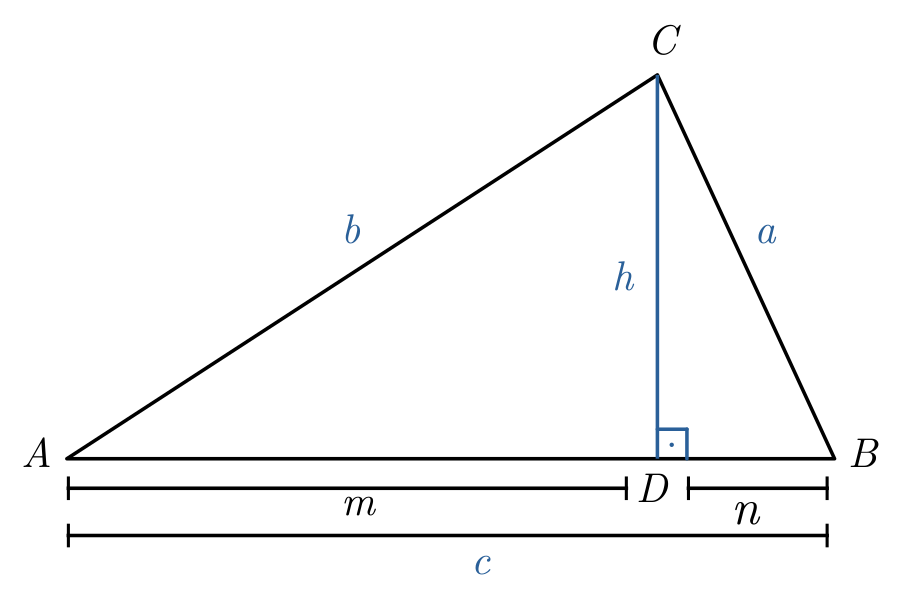
\includegraphics[width=2in]{./cap_fun/dados/fig_leiDosCossenos/fig.png}
  \end{figure}
  Desenvolva um código que computa e imprime o valor da altura de um triangulo de lados $a$, $b$ e $c$ fornecidos por usuária(o).
\end{exer}
\begin{resp}
  Dica: use a \href{https://pt.wikipedia.org/wiki/Lei_dos_cossenos}{lei dos cossenos} e relações fundamentais de triangulo retângulo para obter o valor da altura $h$. 
\end{resp}

\begin{exer}
  Desenvolva um código em que a(o) usuária forneça um ângulo $\theta$ em graus e seja computado e impresso os $\sen(\theta)$ e $\cos(\theta)$.
\end{exer}
\begin{resp}
  Dica: consulte as funções {\PYTHONmathDOTsin}, {\PYTHONmathDOTcos}.
\end{resp}

\begin{exer}
  Desenvolva um jogo em que a(o) usuária(o) tenha três tentativas para adivinhar um número inteiro entre $0$ a $51$ (incluídos). 
\end{exer}
\begin{resp}
  Dica: O módulo {\PYTHONrandom} fornece a função {\PYTHONrandomDOTrandint}\texttt{(a, b)} que retorna um inteiro $a \leq x \leq b$.
\end{resp}

\ifisbook
\subsubsection{Respostas}
\shipoutAnswer
\fi

\section{Definindo Funções}\label{cap_fun_sec_def}

Em {\python}, criamos ou \hl{definimos uma função com a instrução {\PYTHONdef}}, com a seguinte sintaxe

\begin{lstlisting}
def foo(x):
  bloco
\end{lstlisting}

Aqui, \lstinline+foo+ é o nome da função, \lstinline+x+ é o parâmetro (variável) de entrada e \lstinline+bloco+ é o bloco de programação que a função executa ao ser chamada. Uma função pode ter mais parâmetros ou não ter parâmetro de entrada.

\begin{ex}\label{cap_fun_sec_def:ex:areaCirc}
  O seguinte código, define a função \lstinline+areaCirc+ que computa e imprime a área de uma circunferência de raio $r$.

\begin{lstlisting}
import math as m

def areaCirc(r):
  area = m.pi * r**2
  print(f'área = {area}')
\end{lstlisting}

Uma vez definida, a função pode ser chamada em qualquer parte do código. Por exemplo, vamos continuar o código de forma que a(o) usuária(o) informe os raios de duas circunferências e o código compute e imprima o valor das áreas de cada circunferência.

\begin{lstlisting}
import math as m

# def fun
def areaCirc(r):
  area = m.pi * r**2
  print(f'área = {area}')
    
# entrada de dados
raio1 = float(input('Digite o raio da 1. circ.:\n'))
raio2 = float(input('Digite o raio da 2. circ.:\n'))

print(f'Circunferência de raio = {raio1}')
areaCirc(raio1)

print(f'Circunferência de raio = {raio2}')
areaCirc(raio2)
\end{lstlisting}

\end{ex}

\begin{obs}\normalfont{(\hl{\texttt{docstring}}.)}
  {\python} recomenda a utilização do sistema de documentação \lstinline+docstring+. Na definição de funções, um pequeno comentário sobre sua funcionalidade, seguido da descrição sobre seus parâmetros podem ser feito usando \lstinline+'''+, logo abaixo da instrução {\PYTHONdef}. Por exemplo,

\begin{lstlisting}
import math as m

# def fun
def areaCirc(r):
  '''
  Computa e imprime a área de uma
  circunferência.

  Entrada
  -------
  r : float
  Raio da circunferência.
  '''
  area = m.pi * r**2
  print(f'área = {area}')
\end{lstlisting}

Com isso, podemos usar a função {\PYTHONhelp} para obter a documentação da função \lstinline+areaCirc+.

\begin{lstlisting}
>>> help(areaCirc)
\end{lstlisting}

Verifique!
\end{obs}

Uma função pode ser definida sem parâmetro de entrada.

\begin{ex}
  O seguinte código, implementa uma função que imprime um número randômico par entre $0$ e $100$ (incluídos).

\begin{lstlisting}
import random

def randPar100():
  '''
  Imprime um número randômico
  par entre 0 e 100 (incluídos).
  '''
  n = random.randint(0, 99)
  if (n % 2 == 0):
    print(n)
  else:
    print(n+1)
\end{lstlisting}

Para chamá-la, usamos

\begin{lstlisting}
>>> randPar100()
\end{lstlisting}

Verifique!
\end{ex}

\subsection{Funções com Saída de Dados}

Além de parâmetros de entrada, \hl{uma função pode ter saída de dados}, i.e. pode retornar dados para o programa. Para isso, usamos a instrução {\PYTHONreturn} que interrompe a execução da função e retorna ao programa principal. Quando o {\PYTHONreturn} é seguido de um objeto, a função tem como saída o valor desse objeto.

\begin{ex}
  Vamos atualizar a versão de nosso código do Exemplo \ref{cap_fun_sec_def:ex:areaCirc}. Aqui, em vez de imprimir, a função \lstinline+areaCirc(r)+ tem como saída o valor computado da área da circunferência de raio \lstinline+r+

\begin{lstlisting}
import math as m

# def fun
def areaCirc(r):
    area = m.pi * r**2
    return area
    
# entrada de dados
raio1 = float(input('Digite o raio da 1. circ.:\n'))
raio2 = float(input('Digite o raio da 2. circ.:\n'))

print(f'Circunferência de raio = {raio1}')
area1 = areaCirc(raio1)
print(f'\tárea = {area1}')

print(f'Circunferência de raio = {raio2}')
area2 = areaCirc(raio2)
print(f'\tárea = {area2}')
\end{lstlisting}

\end{ex}

Funções podem retornar objetos de qualquer classe de dados. Quando queremos retornar mais de um objeto por vez, usualmente usamos um {\PYTHONtuple} como variável de saída.

\begin{ex}
  O seguinte código, cria uma função para a computação das raízes de um polinômio de grau 2
  \begin{equation}
    p(x) = ax^2 + bx + c.
  \end{equation}

\begin{lstlisting}[caption=raizes\_v1.py, label=cap_progest_sec_def:cod:raizes_v1]
import math as m

def raizes(a, b, c):
  '''
  Computa as raízes de
  p(x) = ax^2 + bx + c

  Entrada
  -------
  a : float
  Coeficiente do termo quadrático.
  Atenção! Deve ser diferente de zero.

  b : float 
  Coeficiente do termo linear.

  c: float
  Coeficiente do termo constante.

  Saída
  -----
  x1 : float
  Uma raiz do polinômio.

  x2 : float
  Outra raiz do polinômio.
  Atenção! No caso de raiz dupla,
  x1 == x2.
  '''

  # auxiliares
  _2a = 2*a
  _b2a = -b/_2a

  # discriminante
  delta = b**2 - 4*a*c

  # raízes
  if (delta > 0):
    x1 = _b2a + m.sqrt(delta)/_2a
    x2 = _b2a - m.sqrt(delta)/_2a
    return x1, x2
  elif (delta < 0):
    img = m.sqrt(-delta)/_2a
    x1 = _b2a + img*1j
    return x1, x1.conjugate()
  else:
    return _b2a, _b2a
\end{lstlisting}
  
Verifique!
\end{ex}

\subsection{Capturando Exceções}

\hl{Exceções são classes de erros encontrados durante a execução de um código}. Ao encontrar uma exceção, a execução do código {\python} é imediatamente interrompida e uma mensagem é impressa indicando a classe do erro e a linha do código em ocorreu. Por exemplo, ao chamarmos \lstinline+raizes(0, 1, 2)+ definida no Código \ref{cap_progest_sec_def:cod:raizes_v1}, obtemos uma exceção da classe \lstinline+ZeroDivisionError+.

\begin{lstlisting}
>>> raizes(0,1,2)
Traceback (most recent call last):
  File "<stdin>", line 1, in <module>
  File "/AlgoritmosProgramacaoI/aux.py", line 33, in raizes
    _b2a = -b/_2a
ZeroDivisionError: division by zero
\end{lstlisting}

Podemos controlar as exceções com a instrução {\PYTHONtry}-{\PYTHONexcept}. Sua sintaxe é

\begin{lstlisting}
try:
  comando1
except:
  comando2
\end{lstlisting}

Ou seja, o código tenta executar o \lstinline+comando1+, caso ele gere uma exceção, o \lstinline+comando2+ é executado. A lista de exceções predefinidas na linguagem pode ser consultada em
\begin{center}
  \url{https://docs.python.org/3/library/exceptions.html}
\end{center}

\begin{ex}
  No Código \ref{cap_progest_sec_def:cod:raizes_v1}, podemos evitar e avisar a(o) usuária(o) da divisão por zero no caso de $a=0$.

\begin{lstlisting}[caption=raizes\_v2.py]
import math as m

def raizes(a, b, c):
  '''
  Computa as raízes de
  p(x) = ax^2 + bx + c

  Entrada
  -------
  a : float
  Coeficiente do termo quadrático.
  Atenção! Deve ser diferente de zero.

  b : float 
  Coeficiente do termo linear.

  c: float
  Coeficiente do termo constante.

  Saída
  -----
  x1 : float
  Uma raiz do polinômio.

  x2 : float
  Outra raiz do polinômio.
  Atenção! No caso de raiz dupla,
  x1 == x2.
  '''

  # auxiliares
  _2a = 2*a

  try:
    _b2a = -b/_2a
  except ZeroDivisionError:
    raise ZeroDivisionError('a deve ser != 0.')

  # discriminante
  delta = b**2 - 4*a*c

  # raízes
  if (delta > 0):
    x1 = _b2a + m.sqrt(delta)/_2a
    x2 = _b2a - m.sqrt(delta)/_2a
    return x1, x2
  elif (delta < 0):
    img = m.sqrt(-delta)/_2a
    x1 = _b2a + img*1j
    return x1, x1.conjugate()
  else:
    return _b2a, _b2a
\end{lstlisting}

\end{ex}

\begin{obs}
  Nos casos gerais, pode-se utilizar a seguinte sintaxe:

\begin{lstlisting}
try:
  comando1
except:
  raise Exception('msg')
\end{lstlisting}

\end{obs}

\subsection{Criando um Módulo}

Para criar um módulo em {\python}, basta escrever um código \lstinline+foo.py+ com as funções e constantes que quisermos. Depois, podemos importá-lo em outro código com a instrução {\PYTHONimport}.

\begin{ex}
  Considere um retângulo de lados $a$ e $b$. Na sequência, temos um módulo com algumas funções.

\begin{lstlisting}[caption=retangulo.py]
'''
Módulo com funcionalidades sobre
retângulos.
'''

import math as m

def perimetro(a, b):
  '''
  Perímetro de um retângulo de 
  lados a e b.

  Entrada
  -------
  a : float
  Comprimento de um dos lados.

  b : float
  Comprimento de outro dos lados.

  Saída
  -----
  p : float
  Perímetro do retângulo.
  '''

  p = 2*a + 2*b
  return p

def area(a, b):
  '''
  Área de um retângulo de 
  lados a e b.

  Entrada
  -------
  a : float
  Comprimento de um dos lados.

  b : float
  Comprimento de outro dos lados.

  Saída
  -----
  area : float
  Área do retângulo.
  '''

  area = a*b
  return area

def diagonal(a, b):
  '''
  Comprimento da diagonal de
  um retângulo de lados a e b.

  Entrada
  -------
  a : float
  Comprimento de um dos lados.

  b : float
  Comprimento de outro dos lados.

  Saída
  -----
  diag : float
  Diagonal do retângulo.
  '''

  diag = m.sqrt(a**2 + b**2)
  return diag
\end{lstlisting}

  Agora, usamos nosso módulo \lstinline+perimetro.py+ em um outro código que fornece informações sobre o retângulo de lados $a$ e $b$ informados por usuária(o).

\begin{lstlisting}
import retangulo as rect

a = float(input('Lado a: '))
b = float(input('Lado b: '))

diag = rect.diagonal(a, b)
print(f'diagonal = {diag}')

perim = rect.perimetro(a, b)
print(f'perímetro = {perim}')

area = rect.area(a, b)
print(f'área = {area}')
\end{lstlisting}

\end{ex}

\subsection{Exercícios}

\begin{exer}
  Defina uma função que recebe os catetos $a$ e $b$ de um triângulo retângulo e retorne o valor de sua hipotenusa. Use-a para escrever um código em que a(o) usuária(o) informa os catetos e obtenha o valor da hipotenusa.
\end{exer}

\begin{exer}
  Defina uma função que recebe os lados $a$, $b$ e $c$ de um triângulo qualquer e retorne o valor de sua área. Use-a para escrever um código em que a(o) usuária(o) informa os lados do triângulo e obtenha o valor da área.  
\end{exer}
\begin{resp}
  Dica: Use o \href{https://pt.wikipedia.org/wiki/Teorema\_de\_Her\%C3\%A3o}{Teorema de Heron}.
\end{resp}

\begin{exer}
  Defina uma função que retorna um número randômico ímpar entre $1$ e $51$ (incluídos). Use-a para escrever um código em que:
  \begin{enumerate}[1.]
  \item A(o) usuária(o) informa um número inteiro $n\geq 1$.
  \item Cria-se uma lista de $n$ números randômicos ímpares entre $1$ e $51$ (incluídos).
  \item Computa-se e imprime-se a média dos $n$ números.
  \end{enumerate}
\end{exer}
\begin{resp}

\begin{lstlisting}
import random

def randImpar(m=51):
  '''
  Retorna um número randômico
  ímpar entre 1 e m (incluídos).

  Entrada
  -------
  m : int
  Maior inteiro ímpar que pode ser 
  gerado. Padrão: m = 51.

  Saída
  -----
  n : int
  Número randômico ímpar.
  '''
  n = random.randint(0, m-1)
  if (n % 2 != 0):
    return n
  else:
    return n+1

# entrada de dados
n = int(input('Digite o tamanho da lista:\n'))

# gera a lista
lista = [0]*n
for i in range(n):
  lista[i] = randImpar()

# calcula a média
soma = sum(lista)
media = soma/len(lista)

# imprime o resultados
print(f'média = {media}')
\end{lstlisting}

\end{resp}

\begin{exer}
  Desenvolva um código para computar a raiz de uma função afim
  \begin{equation}
    f(x) = ax + b,
  \end{equation}
  com coeficientes $a$ e $b$ informados por usuária(o). Use instruções {\PYTHONtry}-{\PYTHONexcept} para monitorar as exceções em que a usuária informe números inválidos ou $a=0$.
\end{exer}
\begin{resp}

\begin{lstlisting}
import math as m

def raizFunAfim(a, b):
  '''
  Computa a raiz de
  f(x) = ax + b

  Entrada
  -------
  a : float
  Coeficiente angular.

  b : float
  Coeficiente linear.

  Saída
  -----
  x : float
  Raiz de f(x).
  '''
  
  try:
    x = -b/a
  except ZeroDivisionError:
    raise ZeroDivisionError('coef. angular deve ser != 0.')

  return x

# entrada de dados
try:
  a = float(input('Coef. angular: '))
except ValueError:
  raise ValueError('Número inválido.')

try:
  b = float(input('Coef. linear: '))
except ValueError:
  raise ValueError('Número inválido.')

# raiz
raiz = raizFunAfim(a, b)

# imprime
print(f'raiz = {raiz}')
\end{lstlisting}

\end{resp}

\begin{exer}
  Considere polinômios de segundo grau
  \begin{equation}
    p(x) = ax^2 + bx + c.
  \end{equation}
  Desenvolva um módulo com as seguintes funções:
  \begin{enumerate}[a)]
  \item \lstinline+intercepta_y()+: função que retorna o ponto de interseção do gráfico de $y = p(x)$ com o eixo das ordenadas\endnote{Eixo $y$.}.
  \item \lstinline+raizes()+: função que retorna as raízes de $p$.
  \item \lstinline+vertice()+: função que retorna o vértice do gráfico de $y=p(x)$.
  \end{enumerate}
  Então, use seu módulo em um código em que a(o) usuária(o) informa os coeficientes $a$, $b$ e $c$ e obtém informações sobre as raízes, o ponto de interseção com o eixo $y$ e o vértice de $p$. 
\end{exer}

\ifisbook
\subsubsection{Respostas}
\shipoutAnswer
\fi


\section{Passagem de Parâmetros}\label{cap_fun_sec_params}

\hl{Uma função pode ter parâmetros de entada}, são as \hl{varáveis} de entrada que são \hl{usadas para que ela receba dados no momento em que é chamada}. Esta estrutura de passar dados para uma função é chamado de passagem de parâmetros. Os parâmetros de entrada são alocados como novas variáveis no chamamento da função e ficam livres ao término de sua execução.

\begin{ex}
  Consideramos o seguinte código:

\begin{lstlisting}
def fun(n):
  print('Na função:')
  print(f'\tn = {n}, id = {id(n)}')
  n = n + 1
  print(f'\tn = {n}, id = {id(n)}')
  return n

n = 1
print(f'n = {n}, id = {id(n)}')

m = fun(n)
print(f'n = {n}, id = {id(n)}')
print(f'm = {m}, id = {id(m)}')
\end{lstlisting}
  
Na linha 10, o identificador \lstinline+n+ é criado com valor 1. Na linha 13, a função \lstinline+fun+ é chamada, um novo identificador \lstinline+n+ é criado apontando para o mesmo valor. No escopo da função (linhas 4-8), apenas este novo \lstinline+n+ é afetado. Ao término da função, este é liberado e o programa principal segue com o identificador \lstinline+n+ original.
\end{ex}

\subsection{Variáveis Globais e Locais}

\hl{Variáveis globais são aquelas que podem ser acessadas por subprogramas} (como funções) e \hl{locais são aquelas que existem somente dentro do escopo de um subprograma}.

\subsubsection{Variáveis Locais}

\hl{Variáveis criadas dentro do escopo de uma função} (incluindo-se os parâmetros de entrada) \hl{são locais}, i.e. só existem durante a execução da função.

\begin{ex}
  Consideramos o seguinte código:

\begin{lstlisting}
def fun(x):
  y = 2*x - 1
  return y

z = fun(2)

try:
  print(f'id(y) = {id(y)}')
except:
  print(f'y não está definida.')
\end{lstlisting}
  
Ao executarmos, imprime-se a mensagem ``y não está definida''. Isto ocorre, pois \lstinline+y+ é variável local na função \lstinline+fun+, é criada e liberada durante sua execução.
\end{ex}

\subsubsection{Variáveis Globais}

\hl{Variáveis definidas no programa principal são globais}, i.e. podem ser acessadas\endnote{Em modo somente leitura.} no escopo de funções, mesmo que não sejam passadas por parâmetros.

\begin{ex}
  Consideramos o seguinte código:

\begin{lstlisting}
x = 3

def fun():
  y = 2*x - 1
  return y

y = fun()
print(f'x = {x}, y = {y}')
\end{lstlisting}
  
A variável \lstinline+x+ é global, i.e. é acessível na função \lstinline+fun+. Execute o código e verifique o valor impresso.
\end{ex}

\hl{A instrução {\PYTHONglobal} permite que variáveis globais possam ser modificadas dentro do escopo de funções}.

\begin{ex}
  Consideramos o seguinte código:

\begin{lstlisting}
def fun():
  global x
  x = x - 1
  y = 2*x - 1
  return y

x = 3
y = fun()
print(f'x = {x}, y = {y}')
\end{lstlisting}

\end{ex}

\subsection{Parâmetros com Valor Padrão}

\hl{Funções podem ter parâmetros com valor padrão}, i.e. no caso que a função ser chamada sem esses parâmetros, eles assumem o valor predefinido na declaração da função.

\begin{ex}
  O seguinte código, imprime uma lista com a Sequência de Fibonacci{\fibonacci}. Por padrão, apenas os cinco primeiros números da sequência são retornados pela função declarada.

\begin{lstlisting}
def bigollo(n=5):
  fibo = [1]*n
  for i in range(2,n):
    fibo[i] = sum(fibo[i-2:i])
  return fibo

print(bigollo())
\end{lstlisting}

\end{ex}

\subsection{Vários Parâmetros}

\hl{Uma função pode ter vários parâmetros de entrada}. A ordem em que os parâmetros são definidos na função devem ser seguidos na passagem de valores. Por exemplo, consideramos a função

\begin{lstlisting}
def fun(x, y):
  print(f'x = {x}')
  print(f'y = {y}')
\end{lstlisting}

Ao chamá-la, devemos passar os valores dos parâmetros \lstinline+x+ e \lstinline+y+ na mesma ordem em que aparecem na definição da função. Por exemplo,

\begin{lstlisting}
>>> fun(1,2)
x = 1
y = 2
\end{lstlisting}

Podemos superar esta restrição, passando os parâmetros de forma explícita. Por exemplo,

\begin{lstlisting}
>>> fun(y=2, x=1)
x = 1
y = 2
\end{lstlisting}

\subsection{Parâmetros Arbitrários}

hl{Uma função pode ter uma quantidade arbitrária de parâmetros}.

\subsubsection{\texttt{tuple} como Parâmetro Arbitrário}

Usa-se a seguinte sintaxe para passar \hl{parâmetros arbitrários com {\PYTHONtuple}}:

\begin{lstlisting}
def fun(*args):
  pass
\end{lstlisting}

\begin{ex}
  Os seguinte código implementa funções para a computação de raízes (reais) de polinômios de até grau 1 e de grau 2.

\begin{lstlisting}
import math as m

def raizPoli1(a, b):
  '''
  ax + b = 0
  '''
  return {-b/a}

def raizPoli2(a, b, c):
  '''
  ax^2 + bx + c = 0
  '''
  delta = b**2 - 4*a*c
  x1 = (-b - m.sqrt(delta))/(2*a)
  x2 = (-b + m.sqrt(delta))/(2*a)
  return {x1, x2}

def raizPoli12(*coefs):
  if (len(coefs) == 2):
    return raizPoli1(coefs[0], coefs[1])
  elif (len(coefs) == 3):
    return raizPoli2(coefs[0], coefs[1], coefs[2])
  else:
    raise Exception('Polinômio inválido.')

print('x - 2 = 0')
print(f'x = {raizPoli12(1,-2)}')

print('2x^2 - 3x + 1 = 0')
print(f'x = {raizPoli12(2, -3, 1)}')
\end{lstlisting}

\end{ex}

\subsubsection{\texttt{dict} como Parâmetros Arbitrários}

Usa-se a seguinte sintaxe para passar \hl{parâmetros arbitrários com {\PYTHONdict}}:

\begin{lstlisting}
def fun(**kwargs):
  pass
\end{lstlisting}


\begin{ex}
  Os seguinte código implementa funções para a computação de raízes (reais) de polinômios de até grau 1 e de grau 2.

\begin{lstlisting}
import math as m

def raizPoli1(a, b):
  '''
  ax + b = 0
  '''
  return {-b/a}

def raizPoli2(a, b, c):
  '''
  ax^2 + bx + c = 0
  '''
  delta = b**2 - 4*a*c
  x1 = (-b - m.sqrt(delta))/(2*a)
  x2 = (-b + m.sqrt(delta))/(2*a)
  return {x1, x2}

def raizPoli12(**coefs):
  if (len(coefs) == 2):
    return raizPoli1(coefs['a'], coefs['b'])
  elif (len(coefs) == 3):
    return raizPoli2(coefs['a'], coefs['b'], coefs['c'])
  else:
    raise Exception('Polinômio inválido.')

print('x - 2 = 0')
print(f'x = {raizPoli12(a=1, b=-2)}')

print('2x^2 - 3x + 1 = 0')
print(f'x = {raizPoli12(a=2, b=-3, c=1)}')
\end{lstlisting}

\end{ex}

\subsection{Exercícios}

\begin{exer}
  Considere o seguinte código:

\begin{lstlisting}
x = 1
def fun(x):
  print(x)
fun(2)
\end{lstlisting}
  
Sem executá-lo, diga qual seria o valor impresso no caso do código ser rodado. Justifique sua resposta.
\end{exer}
\begin{resp}
  2
\end{resp}

\begin{exer}
  Considere o seguinte código:

\begin{lstlisting}
def fun(x):
  global x
  x = x - 1
\end{lstlisting}
  
Ao executá-lo, {\python} gera um erro de sintaxe. Qual é esse erro e por quê ele ocorre?
\end{exer}
\begin{resp}
  Como parâmetro, \lstinline+x+ é variável local, mas está definida como global dentro do escopo da função. Isto causa uma ambiguidade que não é permitida em programas de computadores.
\end{resp}

\begin{exer}
  Considere o seguinte código:

\begin{lstlisting}
y = 1
def fun(x=y):
  y = 2
  print(x)
fun()
\end{lstlisting}
  
Sem executá-lo, diga qual seria o valor impresso no caso de o código ser rodado. Justifique sua resposta.
\end{exer}
\begin{resp}
  1
\end{resp}

\begin{exer}
  Defina uma função {\python} que retorna uma lista com os termos da \href{https://pt.wikipedia.org/wiki/Progress\%C3\%A3o_aritm\%C3\%A9tica}{Progressão Aritmética (P.A.)} $a_i = a_{i-1} + r$, $i = 0, 1, 2, \dotsc, n$. Como parâmetros de entrada, tenha $a_0$ (termo inicial), $r$ (razão da P.A.) e, por padrão, $n = 5$ (número de termos a serem computados).
\end{exer}
\begin{resp}

\begin{lstlisting}
def progAritm(a0, r, n=5):
  return [a0 + i*r for i in range(n+1)]
\end{lstlisting}

\end{resp}

\begin{exer}
  Desenvolva uma função que retorna a lista de números primos entre $n$ e $m$, $m\geq n$. Caso $n$ ou $m$ não sejam fornecidos, a função deve usar $n=1$ e $m=29$ como padrão.
\end{exer}
\begin{resp}

\begin{lstlisting}
def EhPrimo(n):
  info = True
  for i in range(2,n//2+1):
    if (n % i == 0):
      info = False
      break
  return info

def primos(n=1, m=29):
  lista = []
  for x in range(n, m+1):
    if EhPrimo(x):
      lista.append(x)
  return lista
\end{lstlisting}

\end{resp}

\begin{exer}
  Desenvolva uma função que verifica se um ponto pertence a um dado disco
  \begin{equation}
    (x-a)^2 + (y-b)^2 \leq r^2.
  \end{equation}
  Crie-a de forma que ela possa receber uma quantidade arbitrária de pontos para serem verificados. Os parâmetros do disco não sejam informados, ela deve usar, como padrão, o disco unitário com centro na origem.
\end{exer}
\begin{resp}

\begin{lstlisting}
def inDisk(*pts, a=0, b=0, r=1):
  for pt in pts:
    if ((pt[0]-a)**2 + (pt[1]-b)**2 <= r**2):
      print(f'({pt[0]}, {pt[1]}) pertence ao disco.')
    else:
      print(f'({pt[0]}, {pt[1]}) não pertence ao disco.')
\end{lstlisting}

\end{resp}

\ifisbook
\subsubsection{Respostas}
\shipoutAnswer
\fi

\chapter{Arranjos e Matrizes}\label{cap_arr}

\hl{Um arranjo é uma coleção de objetos} (todos de um mesmo tipo) \hl{em que os elementos são organizados por eixos}. É a estrutura de dados mais utilizada para a alocação de vetores e matrizes, fundamentais na computação matricial.

\section{Arranjos}\label{cap_arr_sec_arr}

\hl{Um arranjo (em inglês, \textit{array}) é uma coleção de objetos (todos do mesmo tipo) em que os elementos são organizados por eixos}. Nesta seção, vamos nos restringir a \hl{\emph{arranjos unidimensionais}} (de apenas um eixo). Esta é a estrutura computacionais usualmente utilizada \hl{para a alocação de vetores}.

\hl{{\numpy} é uma biblioteca {\python} que fornece suporte para a alocação e manipulação de arranjos}. Usualmente, a biblioteca é importada como segue

\begin{lstlisting}
import numpy as np
\end{lstlisting}

Na sequência, vamos assumir que o {\numpy} já está importado como acima.

\subsection{Alocação de Arranjos}

O método {\PYTHONnumpyDOTarray} permite a \hl{alocação de um arranjo}. Como parâmetro de entrada, recebe uma {\PYTHONlist} contendo os elementos do arranjo. Por exemplo,

\begin{lstlisting}
>>> v = np.array([-2, 1, 3])
>>> v
array([-2,  1,  3])
>>> type(v)
<class 'numpy.ndarray'>
\end{lstlisting}

aloca o arranjo de números inteiros \lstinline+v+. Embora arranjos não sejam vetores, \hl{a modelagem computacional de vetores usualmente é feita utilizando-se} \texttt{arrays}. Por exemplo, em um código {\python}, o vetor
\begin{equation}
  \pmb{v} = (-2, 1, 3)
\end{equation}
pode ser alocado usando-se o \texttt{array} \lstinline+v+ acima.

O \hl{tipo dos dados} de um \lstinline+array+ é definido na sua criação. Pode ser feita de forma automática ou explícita pela propriedade {\PYTHONnumpyDOTdtype}. Por exemplo,

\begin{lstlisting}
>>> v = np.array([-2, 1, 3])
>>> v.dtype
dtype('int64')
>>> v = np.array([-2., 1, 3])
>>> v.dtype
dtype('float64')
>>> v = np.array([-2, 1, 3], dtype='float')
>>> v.dtype
dtype('float64')
\end{lstlisting}

\begin{ex}
  Aloque o vetor
  \begin{equation}
    \pmb{v} = (\pi, 1, e)
  \end{equation}
  como um \lstinline+array+ do {\numpy}.

\begin{lstlisting}
>>> import numpy as np
>>> v = np.array([np.pi, 1, np.e])
>>> v
array([3.14159265, 1.        , 2.71828183])
\end{lstlisting}

\end{ex}

O {\numpy} conta com \hl{métodos úteis para a \emph{inicialização}} de \texttt{arrays}:
\begin{itemize}
\item {\PYTHONnumpyDOTzeros} \hlemph{arranjo de elementos nulos}

\begin{lstlisting}[xrightmargin=2.5em]
>>> np.zeros(3)
array([0., 0., 0.])
\end{lstlisting}

\item {\PYTHONnumpyDOTones} \hlemph{arranjo de elementos iguais a um}

\begin{lstlisting}[xrightmargin=2.5em]
>>> np.ones(2, dtype='int')
array([1, 1])
\end{lstlisting}

\item {\PYTHONnumpyDOTempty} \hlemph{arranjo de elementos não predefinidos}

\begin{lstlisting}[xrightmargin=2.5em]
>>> np.empty(3)
array([4.64404327e-310, 0.00000000e+000, 6.93315702e-310])
\end{lstlisting}

\item {\PYTHONnumpyDOTlinspace}\texttt{(start, stop, num=50)} \emph{\hl{arranjo de elementos uniformemente espaçados}}

\begin{lstlisting}[xrightmargin=2.5em]
>>> np.linspace(0, 1, 5)
array([0.  , 0.25, 0.5 , 0.75, 1.  ])
\end{lstlisting}
\end{itemize}

\subsection{Indexação e Fatiamento}\label{cap_arr_sec_arr:ssec:islice}

Um {\PYTHONnumpyDOTarray} é uma \hl{coleção de objetos mutável, ordenada e indexada}. Indexação e fatiamento podem ser feitos da mesma forma que para um {\PYTHONtuple} ou uma {\PYTHONlist}. Por exemplo,

\begin{lstlisting}
>>> v = np.array([-1, 1, 2, 0, 3])
>>> v[0]
-1
>>> v[-1]
3
>>> v[1:4]
array([1, 2, 0])
>>> v[::-1]
array([ 3,  0,  2,  1, -1])
>>> v[3] = 4
>>> v
array([-1,  1,  2,  4,  3])
\end{lstlisting}

\subsection{Reordenamento dos Elementos}

Em programação, o reordenamento (em inglês, \textit{sorting}) de elementos de uma sequência ordenada de números (\texttt{array}, \texttt{tuple}, \texttt{tuple}, etc.) consiste em alterar a sequência de forma que os elementos sejam organizados do menor para o mair valor. Na sequência, vamos estudar alguns métodos para isso.

\subsubsection{Método Bolha}

Dado um {\PYTHONnumpyDOTarray}\endnote{Ou, um {\PYTHONtuple}, {\PYTHONlist}, etc..}, o método bolha consiste em percorrer o arranjo e permutar dois elementos consecutivos de forma que o segundo seja sempre maior que o primeiro. Uma vez que percorrermos o arranjo, teremos garantido que o maior valor estará na última posição do arranjo e os demais elementos ainda poderão estar desordenados. Então, percorremos o arranjo novamente, permutando elementos dois-a-dois conforme a ordem desejada, o que trará o segundo maior elemento para a penúltima posição. Ou seja, para um arranjo com $n$ elementos, temos garantido o reordenamento de todos os elementos após $n-1$ repetições desse algoritmo.

\begin{ex}
  Na sequência, implementamos o Método Bolha para o reordenamento de arranjos e aplicamos para
  \begin{equation}
    \pmb{v} = (-1, 1, 0, 4, 3).
  \end{equation}
  
\begin{lstlisting}[caption=bubbleSort\_v1.py]
import numpy as np

def bubbleSort(arr):
  arr = arr.copy()
  n = len(arr)
  for k in range(n-1):
    for i in range(n-k-1):
      if (arr[i] > arr[i+1]):
          arr[i], arr[i+1] = arr[i+1], arr[i]
  return arr

v = np.array([-1,1,0,4,3])
w = bubbleSort(v)
print(w)
\end{lstlisting}

\end{ex}

\begin{obs}
  Em geral, para um arranjo de $n$ elementos, o Método Bolha requer $n-1$ repetições para completar o ordenamento. Entretanto, dependendo do caso, o ordenamento dos elementos pode terminar em menos passos.
\end{obs}

\begin{ex}
  Na sequência, implementamos uma nova versão do Método Bolha para o reordenamento de arranjos. Esta versão verifica se há elementos fora de ordem e, caso não haja, interrompe o algoritmo. Como exemplo, aplicamos para
  \begin{equation}
    \pmb{v} = (-1, 1, 0, 4, 3).
  \end{equation}
  
\begin{lstlisting}[caption=bubbleSort\_v2.py]
import numpy as np

def bubbleSort(arr):
  arr = arr.copy()
  n = len(arr)
  for k in range(n-1):
    noUpdated = True
    for i in range(n-k-1):
      if (arr[i] > arr[i+1]):
        arr[i], arr[i+1] = arr[i+1], arr[i]
        noUpdated = False
    if (noUpdated):
      break
  return arr

v = np.array([-1,1,0,4,3])
w = bubbleSort(v)
\end{lstlisting}

\end{ex}

\begin{obs}\normalfont{(\hl{Métodos de Ordenamento}.)}
  Existem vários métodos para o ordenamento de uma sequência. O Método Bolha é um dos mais simples, mas também, em geral, menos eficiente. O {\numpy} tem disponível a função {\PYTHONnumpyDOTsort} para o reordenamento de elementos. Também bastante útil, é a função {\PYTHONnumpyDOTargsort}, que retorna os índices que reordenam os elementos.
\end{obs}

\subsection{Operações Elemento-a-Elemento}

No {\numpy}, temos os \hlemph{operadores aritméticos elemento-a-elemento} (em ordem de precedência)
\begin{itemize}
\item \lstinline!**!

\begin{lstlisting}[xrightmargin=2.5em]
>>> v = np.array([-2., 1, 3])
>>> w = np.array([1., -1, 2])
>>> v ** w
array([-2.,  1.,  9.])
\end{lstlisting}

\item \lstinline!*!, \lstinline!/!, \lstinline!//!, \lstinline!%!

\begin{lstlisting}[xrightmargin=2.5em]
>>> v * w
array([-2., -1.,  6.])
>>> v / w
array([-2. , -1. ,  1.5])
>>> v // w
array([-2., -1.,  1.])
>>> v % w
array([ 0., -0.,  1.])
\end{lstlisting}

\item \lstinline!+!, \lstinline!-!

\begin{lstlisting}[xrightmargin=2.5em]
>>> v + w
array([-1.,  0.,  5.])
>>> v - w
array([-3.,  2.,  1.])
\end{lstlisting}

\end{itemize}

\begin{ex}
  Vamos usar \texttt{arrays} para alocar os vetores
  \begin{align}
    & \pmb{v} = (1., 0, -2),\\
    & \pmb{w} = (2., -1, 3).
  \end{align}
  Então, computamos o produto interno
  \begin{align}
    & \pmb{v}\cdot\pmb{w} := v_1w_1 + v_2w_2 + v_3w_3 \\
    & \text{}\quad = 1\cdot 2 + 0\cdot(-1) + (-2)\cdot 3 \\
    & \text{}\quad = -4.
  \end{align}

\begin{lstlisting}
import numpy as np
# vetores
v = np.array([1., 0, -2])
w = np.array([2., -1, 3])
# produto interno
vdw = np.sum(v*w)
\end{lstlisting}

\end{ex}

\begin{obs}\normalfont{(\hl{Concatenação de Arranjos}.)}
  No {\numpy}, a concatenação de arranjos pode ser feita com a função {\PYTHONnumpyDOTconcatenate}. Por exemplo,

\begin{lstlisting}
>>> v = np.array([1,2])
>>> w = np.array([3,4])
>>> np.concatenate((v,w))
array([1, 2, 3, 4])
\end{lstlisting}

\end{obs}

\subsection{Exercícios}

\begin{exer}
  Aloque cada um dos seguintes vetores como um {\PYTHONnumpyDOTarray}:
  \begin{enumerate}[a)]
  \item $\displaystyle\pmb{a} = (0, -2, 4)$
  \item $\displaystyle\pmb{b} = (0.1, -2.7, 4.5)$
  \item $\displaystyle\pmb{c} = (e, \ln(2), \pi)$
  \end{enumerate}
\end{exer}
\begin{resp}

\begin{lstlisting}
>>> import numpy as np
>>> a = np.array([0, -2, 4])
>>> b = np.array([0.1, -2.7, 4.5])
>>> c = np.array([np.e, np.log(2), np.pi])
\end{lstlisting}

\end{resp}

\begin{exer}
  Considere o seguinte {\PYTHONnumpyDOTarray}

\begin{lstlisting}
>>> v = np.array([4, -1, 1, -2, 3]).
\end{lstlisting}

Sem implementar, escreva os arranjos derivados:
  \begin{enumerate}[a)]
  \item \lstinline+v[1]+
  \item \lstinline+v[1:4]+
  \item \lstinline+v[:3]+
  \item \lstinline+v[1:]+
  \item \lstinline+v[1:4:2]+
  \item \lstinline+v[-2:-5:-1]+
  \item \lstinline+v[::-2]+
  \end{enumerate}
  Então, verifique seus resultados implementando-os.
\end{exer}
\begin{resp}
  Dica: consulte a Subseção \ref{cap_arr_sec_arr:ssec:islice}. 
\end{resp}

\begin{exer}
  Desenvolva uma função \lstinline+argBubbleSort(arr)+, i.e. uma função que retorna os índices que reordenam os elementos do arranjo \lstinline+arr+ em ordem crescente. Teste seu código para o ordenamento de diversos arranjos e compare os resultados com a aplicação da função {\PYTHONnumpyDOTargsort}.
\end{exer}
\begin{resp}

\begin{lstlisting}
import numpy as np

def argBubbleSort(arr):
  n = len(arr)
  ind = np.arange(n)
  for k in range(n-1):
    noUpdated = True
    for i in range(n-k-1):
      if (arr[ind[i]] > arr[ind[i+1]]):
        ind[i], ind[i+1] = ind[i+1], ind[i]
        noUpdated = False
    if (noUpdated):
      break
  return ind
\end{lstlisting}

\end{resp}

\begin{exer}
  Desenvolva um Método Bolha para o reordenamento dos elementos de um dado arranjo em ordem decrescente. Teste seu código para o reordenamento de diversos arranjos. Como pode-se usar a função {\PYTHONnumpyDOTsort} para obter os mesmos resultados?
\end{exer}
\begin{resp}

\begin{lstlisting}
import numpy as np

def emOrdem(x, y):
    return x < y

def bubbleSort(arr, emOrdem=emOrdem):
  arr = arr.copy()
  n = len(arr)
  for k in range(n-1):
    noUpdated = True
    for i in range(n-k-1):
      if not(emOrdem(arr[i], arr[i+1])):
        arr[i], arr[i+1] = arr[i+1], arr[i]
        noUpdated = False
    if (noUpdated):
        break
  return arr
\end{lstlisting}

\end{resp}

\begin{exer}
  Desenvolva uma função \lstinline+argBubbleSort(arr, emOrdem)+, i.e. uma função que retorna os índices que reordenam os elementos do arranjo \lstinline+arr+ na ordem definida pela função \lstinline+emOrdem+. Teste seu código para o ordenamento de diversos arranjos, tanto em ordem crescente como em ordem decrescente. Como pode-se obter os mesmos resultados usando-se a função {\PYTHONnumpyDOTargsort}?
\end{exer}
\begin{resp}

\begin{lstlisting}
import numpy as np

def argBubbleSort(arr, emOrdem=emOrdem):
  n = len(arr)
  ind = np.arange(n)
  for k in range(n-1):
    noUpdated = True
    for i in range(n-k-1):
      if not(emOrdem(arr[ind[i]], arr[ind[i+1]])):
        ind[i], ind[i+1] = ind[i+1], ind[i]
        noUpdated = False
    if (noUpdated):
      break
  return ind
\end{lstlisting}

\end{resp}

\begin{exer}
  Implemente uma função \lstinline+media(arr)+ que returna o valor médio do arranjo de números \lstinline+arr+. Teste seu código para diferentes arranjos e compare os resultados com o da função {\PYTHONnumpyDOTmean}.
\end{exer}
\begin{resp}

\begin{lstlisting}
import numpy as np

def media(arr):
  return np.sum(arr)/arr.size
\end{lstlisting}

\end{resp}

\begin{exer}
  Desenvolva uma função que retorna o ângulo entre dois vetores $\pmb{v}$ e $\pmb{w}$ dados.
\end{exer}
\begin{resp}

\begin{lstlisting}
import numpy as np

def dot(v, w):
    return np.sum(v*w)

def angulo(v, w):
  # norma de v
  norm_v = np.sqrt(dot(v,v))
  # norma de w
  norm_w = np.sqrt(dot(w,w))
  # cos(theta)
  cosTheta = dot(v,w)/(norm_v*norm_w)
  # theta
  theta = np.acos(cosTheta)
  return theta
\end{lstlisting}

\end{resp}

\ifisbook
\subsubsection{Respostas}
\shipoutAnswer
\fi


\section{Vetores}\label{cap_arr_sec_vetor}

O uso de \texttt{arrays} é uma das formas mais adequadas para fazermos a \hl{modelagem computacional de \emph{vetores}}. Entretanto, devemos ficar atentos que \hl{vetores e arranjos não são equivalentes}. Embora, a soma/subtração e multiplicação por escalar são similares, a multiplicação e potenciação envolvendo vetores não estão definidas, mas para arranjos são operações elemento-a-elemento.

No que segue, vamos assumir que a biblioteca {\numpy} está importada, i.e.

\begin{lstlisting}
>>> import numpy as np
\end{lstlisting}

\begin{ex}
  Podemos alocar os vetores
  \begin{align}
    & \pmb{v} = (1, 0, -2), \\
    & \pmb{w} = (2, -1, 3),
  \end{align}
  como \texttt{arrays} do {\numpy}

\begin{lstlisting}
>>> v = np.array([1, 0, -2])
>>> w = np.array([2, -1, 3])
\end{lstlisting}

  A soma dos vetores é uma operação elemento-a-elemento
  \begin{align}
    & \pmb{v}+\pmb{w} = (1, 0, -2) + (2, -1, 3) \\
    & \text{}\quad = \left(1+2, 0+(-1), -2+3\right) \\
    & \text{}\quad = (3, -1, 1)
  \end{align}
e a dos \texttt{arrays} é equivalente

\begin{lstlisting}
>>> v+w
array([ 3, -1,  1])
\end{lstlisting}

  A subtração dos vetores também é uma operação elemento-a-elemento
  \begin{align}
    & \pmb{v}-\pmb{w} = (1, 0, -2) - (2, -1, 3) \\
    & \text{}\quad = \left(1-2, 0-(-1), -2-3\right) \\
    & \text{}\quad = (-1, 1, -5)
  \end{align}
  e a dos \texttt{arrays} é equivalente

\begin{lstlisting}
>>> v-w
array([ -1, 1,  -5])
\end{lstlisting}

  Ainda, a multiplicação por escalar
  \begin{align}
    & 2\pmb{v} = 2(1, 0, -2) \\
    & \text{}\quad = \left(2\cdot 1, 2\cdot 0, 2\cdot(-2)\right) \\
    & \text{}\quad = (2, 0, -4)
  \end{align}
  também é feita elemento-a-elemento, assim como com \texttt{arrays}

\begin{lstlisting}
>>> 2*v
array([ 2,  0, -4])
\end{lstlisting}

  Agora, para vetores, a multiplicação $\pmb{v}\pmb{w}$, divisão $\pmb{v}/\pmb{w}$, potenciação $\pmb{v}^2$ não são operações definidas. Diferentemente, para arranjos são operações elemento-a-elemento

\begin{lstlisting}
>>> v*w
array([ 2,  0, -6])
>>> v/w
array([ 0.5, -0., -0.66666667])
>>> v**2
array([1, 0, 4])
\end{lstlisting}

\end{ex}

\subsection{Funções Vetoriais}

Funções vetoriais $f:\mathbb{R}^n\to\mathbb{R}^n$ e funcionais $f:\mathbb{R}^n\to\mathbb{R}$ também podem ser adequadamente modeladas com o emprego de \texttt{arrays} do \hl{{\numpy}}. A biblioteca também \hl{conta com várias funções matemáticas predefinidas}, consulte
\begin{center}
  \url{https://numpy.org/doc/stable/reference/routines.math.html}
\end{center}

\begin{ex}\normalfont{(\hl{Função Vetorial}.)}
  A implementação da função vetorial $\pmb{f}:\mathbb{R}^3\to\mathbb{R}^3$
  \begin{equation}
    \pmb{f}(\pmb{x}) = (x_1^2+\sin(x_1), x_2^2+\sin(x_2), x_3^2+\sin(x_3))
  \end{equation}
  para $\pmb{x} = (x_1, x_2, x_3)\in\mathbb{R}^3$, pode ser feita da seguinte forma

\begin{lstlisting}
import numpy as np

def f(x):
  return x**2 + np.sin(x)

# exemplo
x = np.array([0, np.pi, np.pi/2])
print(f'y = {f(x)}')
\end{lstlisting}

Verifique!
\end{ex}

\subsection{Produto Interno}

O \hlemph{produto interno} (ou, produto escalar) é a operação entre vetores $\pmb{v},\pmb{w}\in\mathbb{R}^n$ definida por
\begin{equation}
  \pmb{v}\cdot\pmb{w} := v_1w_1+v_2w_2+\cdots+v_nw_n.
\end{equation}
A função {\PYTHONnumpyDOTdot} computa o produto interno dos \texttt{arrays}.

\begin{ex}
  Consideramos os vetores
  \begin{align}
    & \pmb{v} = (1, 0, -2), \\
    & \pmb{w} = (2, -1, 3).
  \end{align}
  O produto interno desses vetores é
  \begin{align}
  & \pmb{v}\cdot\pmb{w} = v_1w_1 + v_2w_2 + v_3w_3 \\
  & \text{}\quad = 1\cdot 2 + 0\cdot(-1) + (-2)\cdot 3 \\
  & \text{}\quad = 2 + 0 -6 = -4.
  \end{align}
  Usando \texttt{arrays}, temos

\begin{lstlisting}
>>> v = np.array([1, 0, -2])
>>> w = np.array([2, -1, 3])
>>> np.sum(v*w)
-4
>>> np.dot(v,w)
-4
\end{lstlisting}

\end{ex}

\subsection{Norma de Vetores}

A \hl{\emph{norma} $L^2$ de um vetor} $\pmb{v}\in\mathbb{R}^n$ é definida por
\begin{equation}
  \|\pmb{v}\| := \sqrt{v_1^2+v_2^2+\cdots+v_n^2}
\end{equation}
O \hl{submódulo de álgebra linear} {\PYTHONnumpyDOTlinalg} contém a função {\PYTHONnumpyDOTlinalgDOTnorm} para a computação da norma de \texttt{arrays}.

\begin{ex}
  A norma do vetor $\pmb{v} = (3, 0, -4)$ é
  \begin{align}
    & \|\pmb{v}\| = \sqrt{v_1^2 + v_2^2 + v_3^2} \\
    & \text{}\quad = \sqrt{3^2 + 0^2 + (-4)^2} \\
    & \text{}\quad = \sqrt{9 + 0 + 16} \\
    & \text{}\quad = \sqrt{25} = 5.
  \end{align}
  Usando o módulo {\PYTHONnumpyDOTlinalg}, obtemos

\begin{lstlisting}
>>> import numpy as np
>>> import numpy.linalg as npla
>>> v = np.array([3, 0, -4])
>>> np.sqrt(np.dot(v,v))
5.0
>>> npla.norm(v)
5.0
\end{lstlisting}

\end{ex}

\subsection{Produto Vetorial}

O \hl{\emph{produto vetorial}} entre dois vetores $\pmb{v}, \pmb{w}\in\mathbb{R}^3$ é definido por
\begin{align}
  & \pmb{v}\times\pmb{w} :=
                          \begin{vmatrix}
                            \pmb{i} & \pmb{j} & \pmb{k}\\
                            v_1 & v_2 & v_3\\
                            w_1 & w_2 & w_3
                          \end{vmatrix}\\
  & \text{}\quad =
                          \begin{vmatrix}
                            v_2 & v_3\\
                            w_2 & w_3
                          \end{vmatrix}\pmb{i}\\
  & \text{}\qquad - \begin{vmatrix}
                            v_1 & v_3\\
                            w_1 & w_3
                          \end{vmatrix}\pmb{j}\\
  & \text{}\qquad + \begin{vmatrix}
                            v_1 & v_2\\
                            w_1 & w_2
                          \end{vmatrix}\pmb{k}\\
\end{align}
A função {\PYTHONnumpyDOTcross} computa o \hl{produto vetorial} entre \texttt{arrays} (unidimensionais de 3 elementos).

\begin{ex}
  O produto vetorial entre os vetores $\pmb{v} = (1, -2, 1)$ e $\pmb{w} = (0, 2, -1)$ é
  \begin{align}
    & \pmb{v}\times \pmb{w} =
                            \begin{vmatrix}
                              \pmb{i} & \pmb{j} & \pmb{k}\\
                              1 & -2 & 1\\
                              0 & 2 & -1
                            \end{vmatrix}\\
    & \text{}\quad = 0\pmb{i} + \pmb{j} + 2\pmb{k}\\
    & \text{}\quad = (0, 1, 2).
  \end{align}
  Com o {\numpy}, temos

\begin{lstlisting}
>>> v = np.array([1, -2, 1])
>>> w = np.array([0, 2, -1])
>>> np.cross(v,w)
array([0, 1, 2])
\end{lstlisting}

\end{ex}

\subsection{Exercícios}

\begin{exer}
  Considere os seguintes vetores
  \begin{align}
    & \pmb{u} = (2, -1, 1), \\
    & \pmb{v} = (1, -3, 2), \\
    & \pmb{w} = (-2, -1, -3).
  \end{align}
  Usando \texttt{arrays} do {\numpy}, compute:
  \begin{enumerate}[a)]
  \item $\pmb{u}\cdot\pmb{v}$
  \item $\pmb{u}\cdot (2\pmb{v})$
  \item $\pmb{u}\cdot (\pmb{w} + \pmb{v})$
  \item $\pmb{v}\cdot (\pmb{v} - 2\pmb{u})$
  \end{enumerate}
\end{exer}
\begin{resp}
  Dica: use a função $np.dot()$ e verifique as computações calculando os resultados esperados.
\end{resp}

\begin{exer}
  Considere os seguintes vetores
  \begin{align}
    & \pmb{u} = (2, -1, 1), \\
    & \pmb{v} = (1, -3, 2), \\
    & \pmb{w} = (-2, -1, -3).
  \end{align}
  Usando \texttt{arrays} do {\numpy}, compute:
  \begin{enumerate}[a)]
  \item $\|\pmb{u}\|$
  \item $\|\pmb{u} + \pmb{v}\|$
  \item $|\pmb{u}\cdot \pmb{w}|$
  \end{enumerate}
\end{exer}
\begin{resp}
  Dica: use a função {\PYTHONnumpyDOTlinalgDOTnorm} e verifique as computações calculando os resultados esperados.
\end{resp}

\begin{exer}
  Dados vetores $\pmb{u}$ e $\pmb{v}$, temos que
  \begin{equation}
    \pmb{u}\cdot\pmb{v} = \|\pmb{u}\|\|\pmb{v}\|\cos\theta,
  \end{equation}
  onde $\theta$ é o ângulo entre esses vetores. Implemente uma função que recebe dois vetores e retorna o ângulo entre eles. Teste seu código para diferentes vetores.
\end{exer}
\begin{resp}

\begin{lstlisting}
import numpy as np
import numpy.linalg as npla

def angulo(v, w):
  # \|v\|
  norm_v = npla.norm(v)
  # \|w\|
  norm_w = npla.norm(w)
  # u.v
  vdw = np.dot(v, w)
  # cos \theta
  ct = norm_v*norm_w/udw
  return np.acos(ct)
\end{lstlisting}

\end{resp}

\begin{exer}
  A projeção ortogonal do vetor $\pmb{u}$ na direção do vetor $\pmb{v}$ é definida por
  \begin{equation}
    \proj_{\pmb{v}} \pmb{u} := \frac{\pmb{u}\cdot\pmb{v}}{\|\pmb{v}\|^2}\pmb{v}.
  \end{equation}
  Implemente uma função que recebe dois vetores $\pmb{u}$, $\pmb{v}$ e retorne a projeção de $\pmb{u}$ na direção de $\pmb{v}$. Teste seu código para diferentes vetores.
\end{exer}
\begin{resp}

\begin{lstlisting}
import numpy as np
import numpy.linalg as npla

def proj(u, v):
  # \|v\|
  norm_v = npla.norm(v)
  # u.v
  udv = np.dot(u, v)
  # proj_v u
  proj_vu = udv/norm_v**2 * v
  return proj_vu
\end{lstlisting}

\end{resp}

\begin{exer}
  Considere os vetores
  \begin{align}
    & \pmb{u} = (2, -3, 1), \\
    & \pmb{v} = (1, -2, -1).
  \end{align}
  Usando \texttt{arrays} do {\numpy}, compute os seguintes produtos vetoriais:
  \begin{enumerate}[a)]
  \item $\pmb{u}\times\pmb{v}$
  \item $\pmb{v}\times (2\pmb{v})$
  \end{enumerate}
\end{exer}
\begin{resp}
  Dica: use a função {\PYTHONnumpyDOTcross} e verifique as computações calculando os resultados esperados.
\end{resp}

\ifisbook
\subsubsection{Respostas}
\shipoutAnswer
\fi

\section{Arranjos Multidimensionais}\label{cap_arr_sec_multi}

\hl{Um arranjo {\PYTHONnumpyDOTarray} é um tabelamento de elementos de um mesmo tipo}. Os elementos são organizados por eixos indexados (em inglês, \textit{axes}). Enquanto que nas seções anteriores nos restringimos a \texttt{arrays} unidimensionais (de apenas um eixo), aqui, vamos estudar a alocação e manipulação de arranjos de vários eixos.

\subsection{Alocação, Indexação e Fatiamento}

A \hlemph{alocação} de um {\PYTHONnumpyDOTarray} com mais de um eixo pode ser feita usando-se de \hlemph{listas encadeadas}. Por exemplo,

\begin{lstlisting}
>>> import numpy as np
>>> a = np.array([[1,2,3],[4,5,6]])
>>> a
array([[1, 2, 3],
       [4, 5, 6]])
\end{lstlisting}

cria o arranjo \lstinline+a+ de dois eixos, enquanto

\begin{lstlisting}
>>> b = np.array([[[1,2],[3,4]],[[-1,-2],[-3,-4]]])
>>> b
array([[[ 1,  2],
        [ 3,  4]],

       [[-1, -2],
        [-3, -4]]])
\end{lstlisting}

cria o arranjo \lstinline+b+ de três eixos. Para fazer um paralelo com a matemática, o arranjo \lstinline+a+ é similar (mas, não equivalente) a matriz $A = [a_{i,j}]_{i,j=1}^{2,3}$
\begin{equation}
  A =
  \begin{bmatrix}
    1 & 2 & 3\\
    4 & 5 & 6
  \end{bmatrix},
\end{equation}
e o arranjo \lstinline+b+ é similar (mas, não equivalente) ao tensor $B = [b_{i,j,k}]_{i,j,k=1}^{2,2,2}$.

A propriedade \lstinline+.shape+ é um {\PYTHONtuple} contendo o \hl{tamanho de cada eixo}. Por exemplo,

\begin{lstlisting}
>>> a.shape
(2, 3)
>>> a.shape[0]
2
>>> a.shape[1]
3
\end{lstlisting}

informa que \lstinline+a+ tem dois eixos, o primeiro com tamanho $2$ e o segundo com tamanho $3$. Um paralelo com matrizes, dizemos que \lstinline+a+ tem duas linhas e três colunas. No caso do arranjo \lstinline+b+, temos

\begin{lstlisting}
>>> b.shape
(2, 2, 2)
>>> b.shape[2]
2
\end{lstlisting}

o que nos informa tratar-se de um \lstinline+array+ de três eixos, cada um com tamanho $2$.

O número total de elementos de um \lstinline+array+ pode ser obtido do atributo {\PYTHONnumpyDOTndarrayDOTsize}. Por exemplo,

\begin{lstlisting}
a.size, b.size
\end{lstlisting}

\begin{verbatim}
(6, 8)
\end{verbatim}

\hl{Os elementos em um arranjo são \emph{indexados por eixos} e o \emph{fatiamento} também pode ser feito por eixos}. Por exemplo,

\begin{lstlisting}
>>> a
array([[1, 2, 3],
       [4, 5, 6]])
>>> a[1,0]
4
>>> a[0]
array([1, 2, 3])
>>> a[:,1]
array([2, 5])
>>> a[:,2:]
array([[3],
       [6]])
>>> a[1,::-1]
array([6, 5, 4])
\end{lstlisting}

No caso do arranjo \lstinline+b+ de três eixos, temos

\begin{lstlisting}
>>> b
array([[[ 1,  2],
        [ 3,  4]],

       [[-1, -2],
        [-3, -4]]])
>>> b[1,1,0]
-3
>>> b[0,1]
array([3, 4])
>>> b[1,0,::-1]
array([-2, -1])
\end{lstlisting}

\subsection{Inicialização}

O {\numpy} conta com várias funções para a inicialização de \texttt{arrays}, algumas das mais usadas são:
\begin{itemize}
\item {\PYTHONnumpyDOTzeros} \hlemph{inicialização com zeros}

\begin{lstlisting}[xrightmargin=2.5em]
>>> np.zeros((2,3))
array([[0., 0., 0.],
       [0., 0., 0.]])
\end{lstlisting}

\item {\PYTHONnumpyDOTones} \hlemph{inicialização com uns}

\begin{lstlisting}[xrightmargin=2.5em]
>>> np.ones((2,3,2))
array([[[1., 1.],
        [1., 1.],
        [1., 1.]],

       [[1., 1.],
        [1., 1.],
        [1., 1.]]])
\end{lstlisting}

\item {\PYTHONnumpyDOTempty} \hlemph{inicialização com valor da memória}

\begin{lstlisting}[xrightmargin=2.5em]
>>> np.empty((2,1))
array([[5.73021895e-300],
       [6.95260453e-310]])
\end{lstlisting}

\end{itemize}
Observamos que o tamanho dos eixos é passado por um {\PYTHONtuple}.

\subsection{Manipulação}

O {\numpy} contém várias funções para a manipulação de \texttt{arrays}. Algumas das mais usadas são:
\begin{itemize}
\item {\PYTHONnumpyDOTreshape} \hl{reformatação de um arranjo}.

\begin{lstlisting}[xrightmargin=2.5em]
>>> a = np.array([[1,2,3],[4,5,6]])
>>> a.reshape(3,2)
array([[1, 2],
       [3, 4],
       [5, 6]])
>>> a.reshape(-1)
array([1, 2, 3, 4, 5, 6])
\end{lstlisting}

\item {\PYTHONnumpyDOTconcatenate} \hl{concatena um {\PYTHONtuple} de arranjos}.

\begin{lstlisting}[xrightmargin=2.5em]
>>> a = np.array([1,2,3])
>>> b = np.array([4,5,6])
>>> np.concatenate((a,b))
array([1, 2, 3, 4, 5, 6])
>>> a = a.reshape(1,-1)
>>> b = b.reshape(1,-1)
>>> np.concatenate((a,b))
array([[1, 2, 3],
       [4, 5, 6]])
>>> np.concatenate((a,b), axis=1)
array([[1, 2, 3, 4, 5, 6]])
\end{lstlisting}

\end{itemize}

\subsection{Operações e Funções Elementares}

De forma análoga a arranjos unidimensionais, as operações aritméticas e funções elementares são aplicadas elemento-a-elementos em um arranjo. Por exemplo,

\begin{lstlisting}
>>> a = np.array([[0.,1/6],[1/4,1/3]])
>>> b = np.array([[0.,6],[4,3]])
>>> np.sin(np.pi*a*b)
array([[0.0000000e+00, 1.2246468e-16],
       [1.2246468e-16, 1.2246468e-16]])
\end{lstlisting}

\subsubsection{Multiplicação Matriz-Vetor}

Dada uma matriz $A = [a_{i,j}]_{i,j=1}^{n,m}$ e um vetor $\pmb{x} = (x_i)_{i=1}^m$, a \hlemph{multiplicação matriz-vetor} $A\pmb{x}$ é definida por
\begin{align}
  & A\pmb{x} = \begin{bmatrix}
    a_{1,1} & a_{1,2} & \cdots & a_{1,m}\\
    a_{2,1} & a_{2,2} & \cdots & a_{2,m}\\
    \vdots & \vdots & \vdots & \vdots\\
    a_{n,1} & a_{n,2} & \cdots & a_{n,m}
  \end{bmatrix}\begin{bmatrix}
    x_1\\
    x_2\\
    \vdots\\
    x_m
  \end{bmatrix}\\
  & \text{}\quad =
    \begin{bmatrix}
      a_{1,1}x_1 + a_{1,2}x_2 + \cdots + a_{1,m}x_m\\
      a_{2,1}x_1 + a_{2,2}x_2 + \cdots + a_{2,m}x_m\\
      \cdots\\
      a_{n,1}x_1 + a_{n,2}x_2 + \cdots + a_{n,m}x_m
    \end{bmatrix}
\end{align}

\begin{ex}
  Considere a matriz
  \begin{equation}
    A =
    \begin{bmatrix}
      1 & -1 & 2\\
      2 & 1 & 3\\
      0 & 2 & 1
    \end{bmatrix}
  \end{equation}
  e o vetor $\pmb{x} = (-1, 2, 1)$. A multiplicação matriz-vetor é
  \begin{align}
    & A\pmb{x} = \begin{bmatrix}
      1 & -1 & 2\\
      2 & 1 & 3\\
      0 & 2 & 1
    \end{bmatrix}
    \begin{bmatrix}
      -1\\
      2\\
      1
    \end{bmatrix}\\
    & \text{}\quad = (-1, 3, 5)
  \end{align}

\begin{lstlisting}
import numpy as np

def MatrizVetor(A, x):
  n,m = A.shape
  y = np.empty(n)
  for i in range(n):
    y[i] = 0.
    for j in range(m):
      y[i] += A[i,j]*x[j]
  return y

A = np.array([[1, -1, 2],
              [2,  1, 3],
              [0,  2, 1]])
x = np.array([-1, 2, 1])
print(MatrizVetor(A,x))
\end{lstlisting}

\end{ex}

\subsubsection{Multiplicação Matriz-Matriz}

Dadas matrizes $A = [a_{i,j}]_{i,j=1}^{n,p}$ e $B = [b_{i,j}]_{i,j=1}^{p,m}$, a \hlemph{multiplicação matriz-matriz} $AB$ é a matriz $AB = C = [c_{i,j}]_{i,j=1}^{n,m}$ de elementos
\begin{equation}
  c_{i,j} = \sum_{k=1}^{p} a_{i,k}\cdot b_{k,j}.
\end{equation}

\begin{ex}
  Consideramos as matrizes
  \begin{equation}
    A =
    \begin{bmatrix}
      1 & -1 & 2\\
      2 & 1 & 3\\
      0 & 2 & 1
    \end{bmatrix}
  \end{equation}
  \begin{equation}
    B =
    \begin{bmatrix}
      2 & 0\\
      1 & 2\\
      0 & 2
    \end{bmatrix}
  \end{equation}
  A multiplicação matriz-matriz $AB$ é
  \begin{align}
    & AB = \begin{bmatrix}
    1 & -1 & 2\\
    \hleq{2} & \hleq{1} & \hleq{3}\\
    0 & 2 & 1
  \end{bmatrix}\begin{bmatrix}
    2 & \hleq{0}\\
    1 & \hleq{2}\\
    0 & \hleq{2}
  \end{bmatrix}
  & \text{}\quad =
        \begin{bmatrix}
          1 & 2\\
          5 & \hleq{8}\\
          2 & 6
        \end{bmatrix}
  \end{align}

\begin{lstlisting}
def MatrizMatriz(A, B):
  n,p = A.shape
  m = B.shape[1]
  C = np.empty((n,m))
  for i in range(n):
    for j in range(m):
      C[i,j] = 0.
      for k in range(p):
        C[i,j] += A[i,k]*B[k,j]
  return C

A = np.array([[1, -1, 2],
              [2,  1, 3],
              [0,  2, 1]])
B = np.array([[2, 0],
              [1, 2],
              [0, 2]])
print(MatrizMatriz(A,B))
\end{lstlisting}

\end{ex}

\subsection{Exercícios}

\begin{exer}
  Aloque o arranjo que corresponde a matriz
  \begin{equation}
    A =
    \begin{bmatrix}
      -2 & 1 & -4\\
      0  & -3 & 2\\
      -1 & 5 & -7\\
      2 & 3 & 6
    \end{bmatrix}
  \end{equation}
  Sem implementar, forneça a saída das seguintes instruções:
  \begin{enumerate}[a)]
  \item \lstinline+A[2,1]+
  \item \lstinline+A[0,2]+
  \item \lstinline+A[-2,-2]+
  \item \lstinline+A[3]+
  \item \lstinline+A[3:,:]+
  \item \lstinline+A[:,2]+
  \item \lstinline+A[:,1:2]+
  \end{enumerate}
\end{exer}
\begin{resp}
  Dica: aloque o arranjo e implemente as instruções.
\end{resp}

\begin{exer}
  Considere o arranjo

\begin{lstlisting}
A = np.array([[[-1,2,0],
               [3,-2,1],
               [1,-4,2]],
              [[2,-1,0],
               [5,-2,0],
               [2,6,3]],
              [[1,-1,0],
               [7,-2,4],
               [2,-2,1]]])
\end{lstlisting}

Sem implementar, forneça a saída das seguintes instruções:
  \begin{enumerate}[a)]
  \item \lstinline+A[2,0,1]+
  \item \lstinline+A[1,1,0]+
  \item \lstinline+A[2]+
  \item \lstinline+A[1,2]+
  \item \lstinline+A[1:,:2,2]+
  \end{enumerate}
\end{exer}
\begin{resp}
  Dica: aloque o arranjo e implemente as instruções.
\end{resp}

\begin{exer}
  Considere o arranjo

\begin{lstlisting}
>>> a = np.array([[1,2],[5,8],[2,6]])
>>> a
array([[1, 2],
       [5, 8],
       [2, 6]])
\end{lstlisting}

Sem implementar, escreva os seguintes arranjos derivados:
  \begin{enumerate}[a)]
  \item \lstinline+a.reshape(6)+
  \item \lstinline+a.reshape(2,3)+
  \item \lstinline+a.reshape(-1)+
  \item \lstinline+a.reshape(-1,3)+
  \item \lstinline+a.reshape(3,-1)+
  \item \lstinline+a.reshape(4,-1)+
  \end{enumerate}
\end{exer}
\begin{resp}
  Dica: aloque o arranjo e implemente as instruções.
\end{resp}

\begin{exer}
  Considere os arranjos

\begin{lstlisting}
>>> a = np.array([1,2,3]).reshape(1,-1)
>>> b = np.array([4,5,6]).reshape(-1,1)
\end{lstlisting}

Sem implementar, escreva os seguintes arranjos derivados:
  \begin{enumerate}[a)]
  \item \lstinline+np.concatenate((a,b.reshape(1,-1)))+
  \item \lstinline+np.concatenate((a.reshape(-1,1),b))+
  \item \lstinline+np.concatenate((a,b.reshape(1,-1)), axis=1)+
  \item \lstinline+np.concatenate((a.reshape(-1,1),b), axis=1)+
  \end{enumerate}
\end{exer}
\begin{resp}
  Dica: aloque o arranjo e implemente as instruções.
\end{resp}

\begin{exer}
  Implemente uma função que recebe uma matriz (representada por um \lstinline+array+) e retorna a sua transposta. Teste seu código para diversas matrizes com diversos formatos.
\end{exer}
\begin{resp}

\begin{lstlisting}
import numpy as np

def Transposta(A):
  n,m = A.shape
  B = np.empty((m,n))
  for i in range(n):
    for j in range(m):
      B[j,i] = A[i,j]
  return B
\end{lstlisting}

\end{resp}

\begin{exer}
  Implemente uma função que compute a multiplicação vetor-matriz
  \begin{align}
    & \pmb{y} = \pmb{x}A \\
    & \text{}\quad := \begin{bmatrix}
              x_1 & x_2 & \cdots & x_n
            \end{bmatrix}
            \begin{bmatrix}
              a_{1,1} & a_{1,2} & \cdots & a_{1,m}\\
              a_{2,1} & a_{2,2} & \cdots & a_{2,m}\\
              \vdots & \vdots & \vdots & \vdots\\
              a_{n,1} & a_{n,2} & \cdots & a_{n,m}
            \end{bmatrix}
  \end{align}
  onde, por definição, $\pmb{y} = [y_j]_{j=1}^m$, com elementos
  \begin{equation}
    y_j = \sum_{k=1}^n x_k\cdot a_{k,j}.
  \end{equation}
\end{exer}
\begin{resp}
  Dica: a função {\PYTHONnumpyDOTdot} também computa a multiplicação vetor-matriz. Teste sua implementação para diferentes matriz e vetores de diferentes tamanhos.
\end{resp}

\ifisbook
\subsubsection{Respostas}
\shipoutAnswer
\fi


\section{Matrizes}\label{cap_arr_sec_mat}

Arranjos multidimensionais\endnote{Consulte a Seção \ref{cap_arr_sec_multi}} fornecem uma estrutura adequada para a representação de matrizes em computador. \hl{Uma matriz $A$, assim como um arranjo bidimensional, é uma coleção de valores organizados de forma retangular}, por exemplo, a matriz $A = [a_{i,j}]_{i,j=1}^{n,m}$ tem a forma
\begin{equation}\hleq
  A =
  \begin{bmatrix}
    a_{1,1} & a_{1,2} & \cdots & a_{1,m}\\
    a_{2,1} & a_{2,2} & \cdots & a_{2,m}\\
    \vdots & \vdots & \vdots & \vdots\\
    a_{n,1} & a_{n,2} & \cdots & a_{n,m}
  \end{bmatrix}
\end{equation}
Seus elementos $a_{i,j}$ são organizados por eixos, o eixo das linhas (\lstinline+axis=0+) e o eixo das colunas (\lstinline+axis=1+).

\begin{ex}\label{cap_arr_sec_mat:ex:sislin}
  O sistema linear
  \begin{subequations}
    \begin{align}
      & 2x_1 - x_2 + x_3 = -3 \\
      & -x_1 + x_2 + {\hleq 3}x_3 = {\hleq 6} \\
      & x_1 + 3x_2 - 3x_3 = 2
    \end{align}
  \end{subequations}
  pode ser escrito na seguinte forma matricial
  \begin{equation}
    A\pmb{x} = \pmb{b},
  \end{equation}
  onde $A = [a_{i,j}]_{i,j=1}^{3,3}$ é a matriz de coeficientes
  \begin{equation}
    A =
    \begin{bmatrix}
      2 & -1 & 1\\
      -1 & 1 & {\hleq 3}\\
      1 & 3 & -3
    \end{bmatrix},
  \end{equation}
  o vetor dos termos constantes $\pmb{b} = (b_1, b_2, b_3)$ é
  \begin{equation}
    \pmb{b} = (-3, {\hleq 6}, 2),
  \end{equation}
  enquanto que o vetor das incógnitas é $\pmb{x} = (x_1, x_2, x_3)$. No seguinte código, usamos {\PYTHONnumpyDOTarray} para alocamos a matriz dos coeficientes $A$ e o vetor dos termos constantes $\pmb{b}$.

\begin{lstlisting}
import numpy as np
# matriz dos coefs
A = np.array([[2, -1, 1],
              [-1, 1, 3],
              [1, 3, -3]])
# vet termos consts
b = np.array([-3, 6, 2])
\end{lstlisting}

\end{ex}

\subsection{Operações Matriciais}

Embora úteis para a representação de matrizes, \hl{arranjos bidimensionais não são equivalentes a matrizes}. Em arranjos, as operações aritméticas elementares (\lstinline!+!, \lstinline!-!, \lstinline!*!, \lstinline!/!, etc.) são operações elemento-a-elemento, para matrizes a multiplicação não é assim calculada e a divisão não é definida.

\subsubsection{Multiplicação Matricial}

No {\numpy}, as funções {\PYTHONnumpyDOTdot}, {\PYTHONnumpyDOTmatmul} ou o operador \lstinline+@+ podem ser usados para computar a multiplicação matricial.

\begin{ex}
  Considerando as matrizes
  \begin{equation}
    A =
    \begin{bmatrix}
      2 & -1 & 1\\
      -1 & 1 & {\hleq 3}\\
      1 & 3 & -3
    \end{bmatrix},
  \end{equation}
  \begin{equation}
    B =
    \begin{bmatrix}
      1 & -1\\
      2 & 1\\
      1 & 0
    \end{bmatrix}
  \end{equation}
  temos
  \begin{equation}
    AB =
    \begin{bmatrix}
      1 & -3\\
      4 & 2\\
      4 & 2
    \end{bmatrix}
  \end{equation}
  Usando o {\numpy}, temos

\begin{lstlisting}
import numpy as np

A = np.array([[2, -1, 1],
              [-1, 1, 3],
              [1, 3, -3]])

B = np.array([[1, -1],
              [2, 1],
              [1, 0]])

AB = A@B
print(f'AB =\n {AB}')

AB = np.matmul(A, B)
print(f'AB =\n {AB}')

AB = np.dot(A, B)
print(f'AB =\n {AB}')
\end{lstlisting}

\end{ex}

\begin{ex}
  Consideramos o sistema linear introduzido no Exemplo \ref{cap_arr_sec_mat:ex:sislin}. Vamos verificar que sua solução é $x_1 = -1$, $x_2 = 2$ e $x_3 = 1$. Equivalentemente, temos que
  \begin{equation}
    A\pmb{x} = \pmb{b},
  \end{equation}
  com $\pmb{x} = (-1, 2, 1)$. Isto é, se $\pmb{x}$ é solução do sistema, então é nulo o resíduo $\pmb{b} - A\pmb{x}$, i.e.
  \begin{equation}
    \pmb{b} - A\pmb{x} = \pmb{0}.
  \end{equation}
  Ou equivalentemente, $\|\pmb{b} - A\pmb{x}\| = 0$.

\begin{lstlisting}
import numpy as np
import numpy.linalg as npla

# matriz dos coefs
A = np.array([[2, -1, 1],
              [-1, 1, 3],
              [1, 3, -3]])
# vet termos consts
b = np.array([-3, 6, 2])
# solução
x = np.array([-1, 2, 1])

# verificação
res = b - A@x
norm_res = npla.norm(res)
print(f'É solução? {np.isclose(norm_res, 0.)}')
\end{lstlisting}

\end{ex}

\subsubsection{Matriz Transposta}

Por definição, a transposta de uma matriz $A = [a_{i,j}]_{i,j=1}^{n,m}$ é a matriz $A^T = [a_{j,i}]_{j,i=1}^{m,n}$, i.e. a matriz $B$ obtida de $A$ pela permutação de suas linhas com suas colunas. No {\numpy}, a transposta de um arranjo bidimensional pode ser calculado com a função {\PYTHONnumpyDOTtranspose}, com o método {\PYTHONnumpyDOTndarrayDOTtranspose} ou com o atributo {\PYTHONnumpyDOTndarrayDOTT}.

\begin{ex}
  Uma matriz é dita ser simétrica, quando $A = A^T$. Observamos que é simétrica a matriz
  \begin{equation}
    A =
    \begin{bmatrix}
      2 & -1 & 1\\
      -1 & 1 & {\hleq 3}\\
      1 & 3 & -3
    \end{bmatrix},
  \end{equation}

\begin{lstlisting}
import numpy as np
A = np.array([[2, -1, 1],
              [-1, 1, 3],
              [1, 3, -3]])

trans_A = np.transpose(A) 
print(f'A^T =\n {trans_A}')

trans_A = A.transpose() 
print(f'A^T =\n {trans_A}')

trans_A = A.T
print(f'A^T =\n {trans_A}')

print(f'É simétrica? {np.allclose(A, A.T)}')
\end{lstlisting}

Agora, não é simétrica a matriz
  \begin{equation}
    B =
    \begin{bmatrix}
      1 & -1\\
      2 & 1\\
      1 & 0
    \end{bmatrix}.
  \end{equation}

\begin{lstlisting}
import numpy as np
B = np.array([[1, -1],
              [2, 1],
              [1, 0]])
print(B.T)
\end{lstlisting}

\end{ex}

\subsubsection{Determinante}

Por definição, o determinante de uma matriz $A = [a_{i,j}]_{i,j=1}^{n,n}$ é o escalar
\begin{align}
  & \det(A) =
            \begin{vmatrix}
              a_{1,1} & a_{1,2} & \cdots & a_{1,n}\\
              a_{2,1} & a_{2,2} & \cdots & a_{2,n}\\
              \vdots & \vdots & \vdots & \vdots\\
              a_{n,1} & a_{n,2} & \cdots & a_{n,n}                
            \end{vmatrix}\\
  & \text{}\quad := \sum_{\sigma\in S_n}\sign(\sigma)a_{1,\sigma_1}a_{2,\sigma_2}\cdots a_{n,\sigma_n}
\end{align}
onde $S_n$ é o conjunto de todas as permutações de ${1, 2, \dotsc, n}$ e $\sign(\sigma)$ é o sinal (ou assinatura) da permutação $\sigma\in S_n$. Para matrizes $2\times 2$, temos
\begin{align}
  & \det(A) =
      \begin{vmatrix}
        a_{1,1} & a_{1,2}\\
        a_{2,1} & a_{2,2}
      \end{vmatrix}\\
  & \text{}\quad = a_{1,1}a_{2,2} - a_{1,2}a_{2,1}.
\end{align}
Enquanto que no caso de matriz $3\times 3$, temos
\begin{align}
  & \det(A) =
            \begin{vmatrix}
              a_{1,1} & a_{1,2} & a_{1,3}\\
              a_{2,1} & a_{2,2} & a_{2,3}\\
              a_{3,1} & a_{3,2} & a_{3,3}
            \end{vmatrix}\\
  & \text{}\quad = a_{1,1}a_{2,2}a_{3,3}\\
  & \text{}\qquad + a_{1,2}a_{2,3}a_{3,1}\\
  & \text{}\qquad + a_{1,3}a_{2,1}a_{3,2}\\
  & \text{}\qquad - a_{1,3}a_{2,2}a_{3,1}\\
  & \text{}\qquad - a_{1,1}a_{2,3}a_{3,2}\\
  & \text{}\qquad - a_{1,2}a_{2,1}a_{3,3}.
\end{align}

A função {\PYTHONnumpyDOTlinalgDOTdet} do {\numpy} pode ser usado para computar o determinante de um arranjo.

\begin{ex}
  O determinante
  \begin{align}
    & \det(A) =
              \begin{vmatrix}
                2 & -1 & 1\\
                -1 & 1 & {\hleq 3}\\
                1 & 3 & -3
              \end{vmatrix}\\
    & \text{}\quad = -28
  \end{align}

\begin{lstlisting}
import numpy as np
import numpy.linalg as npla
A = np.array([[2, -1, 1],
              [-1, 1, 3],
              [1, 3, -3]])

detA = npla.det(A)
print(f'det(A) = {detA}')
\end{lstlisting}

\end{ex}

\subsection{Aplicação: Método de Cramer}

O \hl{\emph{Método de Cramer}}{\cramer} usa de determinantes para o \hl{cálculo da solução de sistemas lineares}. Dado um sistema linear $n\times n$
\begin{equation}\hleq
  A\pmb{x} = \pmb{b}
\end{equation}
denotamos a matriz dos coeficientes por
\begin{equation}
  A =
  \begin{bmatrix}
    \pmb{a}_1 & \pmb{a}_2 & \cdots & \pmb{a}_n
\end{bmatrix},
\end{equation}
onde $\pmb{a}_i$ denota a $i$-ésima coluna de $A$. Vamos denotar por $A_i$ a matriz obtida de $A$ substituindo $\pmb{a}_i$ pelo vetor dos termos constantes $\pmb{b}$, i.e.
\begin{equation}
  A_i :=
  \begin{bmatrix}
    \pmb{a}_1 & \cdots & \pmb{a}_{i-1} & {\hleq \pmb{b}} & \pmb{a}_{i+1} & \cdots & \pmb{a}_n
  \end{bmatrix}
\end{equation}
\hl{O método consiste em computar a solução $\pmb{x} = (x_1, x_2, \ldots, x_n)$ com}
\begin{equation}\hleq
  x_i = \frac{\det(A_i)}{\det(A)},
\end{equation}
para cada $i = 1, 2, \dotsc, n$.

\begin{ex}
  Vamos resolver o sistema linear dado no Exercício \ref{cap_arr_sec_mat:ex:sislin}. Sua forma matricial é
  \begin{equation}
    A\pmb{x} = \pmb{b}
  \end{equation}
  com matriz dos coeficientes
  \begin{equation}
        A =
    \begin{bmatrix}
      2 & -1 & 1\\
      -1 & 1 & 3\\
      1 & 3 & -3
    \end{bmatrix},
  \end{equation}
  e vetor dos termos constantes
  \begin{equation}
    \pmb{b} = ({\hleq -3, ~6, ~2}).
  \end{equation}
  Para aplicação do Método de Cramer, calculamos
  \begin{align}
    & \det(A) :=
              \begin{vmatrix}
                2 & -1 & 1\\
                -1 & 1 & 3\\
                1 & 3 & -3
              \end{vmatrix}\\
    & \text{}\quad = -28
  \end{align}
  e das matrizes auxiliares
  \begin{align}
    & \det(A_1) :=
              \begin{vmatrix}
                {\hleq -3} & -1 & 1\\
                {\hleq 6} & 1 & 3\\
                {\hleq 2} & 3 & -3
              \end{vmatrix}\\
    & \text{}\quad = 28
  \end{align}
  \begin{align}
    & \det(A_2) :=
              \begin{vmatrix}
                2 & {\hleq -3} & 1\\
                -1 & {\hleq 6} & 3\\
                1 & {\hleq 2} & -3
              \end{vmatrix}\\
    & \text{}\quad = -56
  \end{align}
  \begin{align}
    & \det(A_3) :=
              \begin{vmatrix}
                2 & -1 & {\hleq -3}\\
                -1 & 1 & {\hleq 6}\\
                1 & 3 & {\hleq 2}
              \end{vmatrix}\\
    & \text{}\quad = -28
  \end{align}
  Com isso, obtemos a solução
  \begin{align}
    & x_1 = \frac{\det(A_1)}{\det(A)} = -1, \\
    & x_2 = \frac{\det(A_2)}{\det(A)} = 2, \\
    & x_3 = \frac{\det(A_3)}{\det(A)} = 1.
  \end{align}

\begin{lstlisting}
import numpy as np
import numpy.linalg as npla
# matriz dos coefs
A = np.array([[2, -1, 1],
              [-1, 1, 3],
              [1, 3, -3]])
# vet termos consts
b = np.array([-3, 6, 2])

# det(A)
detA = npla.det(A)
print(f'det(A) = {detA}')

# matrizes auxiliares
## A1
A1 = np.copy(A)
A1[:,0] = b
detA1 = npla.det(A1)
print(f'det(A1) = {detA1}')

## A2
A2 = np.copy(A)
A2[:,1] = b
detA2 = npla.det(A2)
print(f'det(A2) = {detA2}')

## A3
A3 = np.copy(A)
A3[:,2] = b
detA3 = npla.det(A3)
print(f'det(A3) = {detA3}')

# solução
x = np.array([detA1/detA, detA2/detA, detA3/detA])
print(f'x = {x}')
\end{lstlisting}

\end{ex}


\subsection{Exercícios}

\begin{exer}
  Aloque com {\PYTHONnumpyDOTarray} e imprima as seguintes matrizes:
  \begin{enumerate}[a)]
  \item
    \begin{equation}
      A =
      \begin{bmatrix}
        -1 & 2\\
        7 & -3
      \end{bmatrix}
    \end{equation}
  \item
    \begin{equation}
      B =
      \begin{bmatrix}
        -1 & 2 & 4\\
        7 & -3 & -5 
      \end{bmatrix}
    \end{equation}
  \item
    \begin{equation}
      C =
      \begin{bmatrix}
        -1 & 2 & 4\\
        7 & -3 & -5\\
        2 & 9 & 6
      \end{bmatrix}
    \end{equation}
  \item
    \begin{equation}
      D =
      \begin{bmatrix}
        -1 & 2 & 4\\
        7 & -3 & -5\\
        2 & 9 & 6\\
        1 & -1 & 1
      \end{bmatrix}
    \end{equation}
  \end{enumerate}
\end{exer}
\begin{resp}

\begin{lstlisting}
import numpy as np
# a)
A = np.array([[-1, 2],
              [7, -3]])
print(f'A =\n {A}')
# b)
B = np.array([[-1, 2, 4],
              [7, -3, -5]])
print(f'B =\n {B}')
# c)
C = np.array([[-1, 2, 4],
              [7, -3, -5],
              [2, 9, 6]])
print(f'C =\n {C}')
# d)
D = np.array([[-1, 2, 4],
              [7, -3, -5],
              [2, 9, 6],
              [1, -1, 1]])
print(f'D =\n {D}')
\end{lstlisting}

\end{resp}

\begin{exer}
  Aloque as seguintes matrizes com {\PYTHONnumpyDOTarray}
  \begin{equation}
    A =
    \begin{bmatrix}
        -1 & 2 & 4\\
        7 & -3 & -5
      \end{bmatrix}      
  \end{equation}
  e
  \begin{equation}
    B =
    \begin{bmatrix}
        1 & -1 & 2\\
        3 & 0 & 5
      \end{bmatrix}.      
  \end{equation}
  Então, compute e imprima o resultado das seguintes operações matriciais
  \begin{enumerate}[a)]
  \item $A + B$
  \item $A - B$
  \item $2A$
  \end{enumerate}
\end{exer}
\begin{resp}

\begin{lstlisting}
import numpy as np
A = np.array([[-1, 2, 4],
              [7, -3, -5]])
B = np.array([[1, -1, 2],
              [3, 0, 5]])
# a)
ApB = A + B
print(f'A+B =\n {ApB}')
# b)
AmB = A - B
print(f'A-B =\n {AmB}')
# c)
_2A = 2*A
print(f'2A =\n {_2A}')
\end{lstlisting}

\end{resp}

\begin{exer}
  Aloque as seguintes matrizes {\PYTHONnumpyDOTarray}:
  \begin{equation}
    A =
    \begin{bmatrix}
        -1 & 2 & 4\\
        7 & -3 & -5
      \end{bmatrix}      
  \end{equation}
  e
  \begin{equation}
    B =
    \begin{bmatrix}
        1 & -1\\
        3 & 0\\
        2 & 5
      \end{bmatrix}.      
  \end{equation}
  Então, compute e imprima o resultado das seguintes operações matriciais:
  \begin{enumerate}[a)]
  \item $AB$
  \item $BA$
  \item $B^T$
  \item $A^TB^T$
  \end{enumerate}
\end{exer}
\begin{resp}

\begin{lstlisting}
import numpy as np
A = np.array([[-1, 2, 4],
              [7, -3, -5]])
B = np.array([[1, -1],
              [3, 0],
              [2, 5]])
# a)
AB = A @ B
print(f'AB =\n {AB}')
# b)
BA = B @ A
print(f'BA =\n {BA}')
# c)
Bt = B.T
print(f'B^T =\n {Bt}')
# d)
AtBt = A.T @ B.T
print(f'A^T.B^T =\n {AtBt}')
\end{lstlisting}

\end{resp}

\begin{exer}\label{cap_arr_sec_mat:exer:sislin}
  Escreva a forma matricial $A\pmb{x} = \pmb{b}$ do seguinte sistema linear
  \begin{subequations}
    \begin{align}
      & -x_1 + 2x_2 - 2x_3 = 6 \\
      & 3x_1 - 4x_2 + x_3 = -11 \\
      & x_1 -5x_2 + 3x_3 = -10
    \end{align}
  \end{subequations}
  Use {\PYTHONnumpyDOTarray} para alocar a matriz dos coeficientes $A$ e o vetor dos termos constantes $\pmb{b}$. Então, verifique quais dos seguintes vetores é solução do sistema
  \begin{enumerate}[a)]
  \item $\pmb{x} = (1, -1, -2)$
  \item $\pmb{x} = (-1, -2, 1)$
  \item $\pmb{x} = (-2, 1, -1)$
  \end{enumerate}
\end{exer}
\begin{resp}

\begin{lstlisting}
import numpy as np
A = np.array([[-1, 2, -2],
              [3, -4, 1],
              [1, -5, 3]])
b = np.array([6, -11, -10])
# c)
x = np.array([-2, 1, -1])
print(f'É solução? {np.allclose(A@x, b)}')
\end{lstlisting}

\end{resp}

\begin{exer}
  Calcule e compute o determinante das seguintes matrizes
  \begin{enumerate}[a)]
  \item
    \begin{equation}
      A =
      \begin{bmatrix}
        -1 & 2\\
        7 & -3
      \end{bmatrix}
    \end{equation}
  \item
    \begin{equation}
      B =
      \begin{bmatrix}
        -1 & 2 & 4\\
        1 & -3 & -5\\
        2 & 0 & 6
      \end{bmatrix}
    \end{equation}
  \item
    \begin{equation}
      C =
      \begin{bmatrix}
        -1 & 2 & 4 & 1\\
        7 & -3 & -5 & -1\\
        2 & 0 & 1 & 0\\
        1 & -1 & 1 & -2
      \end{bmatrix}
    \end{equation}
  \end{enumerate}
\end{exer}
\begin{resp}

\begin{lstlisting}
import numpy as np
import numpy.linalg as npla
# a)
A = np.array([[-1, 2],
              [7, -3]])
detA = npla.det(A)
print(f'det(A) =\n {detA}')
# b)
B = np.array([[-1, 2, 4],
              [1, -3, -5],
              [2, 0, 6]])
detB = npla.det(B)
print(f'det(B) =\n {detB}')
# c)
C = np.array([[-1, 2, 4, 1],
              [-1, -3, -5, -1],
              [2, 0, 1, 0],
              [1, -1, 1, -2]])
detC = npla.det(C)
print(f'det(C) =\n {detC}')
\end{lstlisting}

\end{resp}

\begin{exer}
  Use o Método de Cramer para computar a solução do sistema dado no Exercício \ref{cap_arr_sec_mat:exer:sislin}. Verifique sua solução com a computada pelo método {\PYTHONnumpyDOTlinalgDOTsolve}.
\end{exer}
\begin{resp}
  Dica: $\pmb{x} = (-2, 1, -1)$.
\end{resp}

\begin{exer}
  Desenvolva sua própria função {\python} para a computação do determinante de uma matriz $A$ $n\times n$.
\end{exer}
\begin{resp}
  Dica: use a função {\PYTHONintertoolsDOTpermutations} para obter um iterador sobre as permutações.
\end{resp}

\ifisbook
\subsubsection{Respostas}
\shipoutAnswer
\fi

\chapter{Arquivos e Gráficos}\label{cap_ag}

\section{Arquivos}\label{cap_ag_sec_arq}

\subsection{Arquivo Texto}

\hl{Um \emph{arquivo texto} usualmente é identificado com a extensão \texttt{.txt} e contém uma \texttt{string}}, i.e. uma coleção de caracteres. 

Consideramos que o seguinte arquivo:

\begin{lstlisting}[caption = foo.txt, label=cap_ag_sec_arq:cod:foo.txt]
'''
Tabela de valores de
y = log(x).
'''

n, x, y
1, 1.0, 0.0000
2, 1.5, 0.4055
3, 2.0, 0.6931
4, 2.5, 0.9163
\end{lstlisting}

O nome deste aquivo é \texttt{foo.txt}. Escreva-o em um editor de texto e salve-o com o nome \texttt{foo.txt} em uma pasta de sua área de usuário no sistema de seu computador.

\subsubsection{Leitura}

\hl{Em programação, a \emph{leitura de um arquivo} consiste em importar dados/informação de um arquivo para um código/programa}. Para tanto, precisamos \hlemph{abrir o arquivo}, i.e. criar um objeto {\PYTHONfile} associado ao arquivo. Em {\python}, abrimos um arquivo com a função {\PYTHONopen}\texttt{(file, mode)}. Nela, \texttt{file} consiste em uma \lstinline+string+ com o \emph{caminho para o aquivo} no sistema de arquivo do sistema operacional e, \texttt{mode} é uma string que especifica o modo de abertura. Para a abertura em modo leitura de um arquivo texto, usa-se \texttt{mode='r'} (\texttt{r}, do inglês, \textit{read}).

Um vez aberto a \hlemph{leitura do arquivo} pode ser feita com métodos específicos do objeto {\PYTHONfile}, por exemplo, com o método {\PYTHONfileDOTread}. Para uma lista de métodos disponíveis em {\python}, consulte
\begin{center}
  \url{https://docs.python.org/3/tutorial/inputoutput.html#methods-of-file-objects}
\end{center}
Por fim, precisamos \hlemph{fechar o arquivo}, o que pode ser feito com o método {\PYTHONfileDOTclose}.

Por exemplo, consideramos o seguinte código

\begin{lstlisting}
fl = open('foo.txt', 'r')
texto = fl.read()
fl.close()
print(texto)
\end{lstlisting}

Na primeira linha, o código: 1. abre o arquivo \texttt{foo.txt}\endnote{Aqui, é considerado que o arquivo está na mesma pasta em que o código está sendo executado.}, 2. lê o aquivo inteiro, 3. fecha-o e, 4. imprime o conteúdo lido. No código, \texttt{texto} é uma \texttt{string} que pode ser manipulada com os métodos e técnicas na Seção~\ref{cap_lingua_sec_string}.

Alternativamente, pode-se fazer a \hlemph{leitura linha-por-linha} do arquivo, como segue

\begin{lstlisting}
fl = open('foo.txt', 'r')
for linha in fl:
  print(linha)
fl.close()
\end{lstlisting}

\subsubsection{Escrita}

\hl{A \emph{escrita de um arquivo} consiste em exportar dados/informações de um código/programa para um arquivo de dados}. Para tanto: 1. abrimos o arquivo no código com o comando {\PYTHONopen}\texttt{(file, mode='w')} (\texttt{w}, do inglês, \textit{write}); 2. usamos um método de escrita, por exemplo, {\PYTHONfileDOTwrite} para escrever no arquivo; 3. fechamos o arquivo com {\PYTHONfileDOTclose}.

Por exemplo, o seguinte código escreve o arquivo \texttt{foo.txt} (consulte o Código~\ref{cap_ag_sec_arq:cod:foo.txt}).

\begin{lstlisting}[caption=foo.py, label=cap_ag_sec_arq:cod:foo.py]
import numpy as np
# abre o arq
fl = open('foo.txt', mode='w')
# cabeçalho
fl.write("""'''
Tabela de valores de
y = log(x)
'''\n""")
# linha em branco
fl.write('\n')
# id das entradas
fl.write('n, x, y\n')
# entradas da tabela
xx = np.arange(1., 3., 0.5)
for i,x in enumerate(xx):
  fl.write(f'{i+1}, {x:.1f}, {np.log(x):.4f}\n')
# fecha o arq
fl.close()
\end{lstlisting}

Observamos que abertura de arquivo no modo \texttt{mode='w'} sobrescreve o arquivo caso ele já exista. Para \hl{escrever em um arquivo já existente}, sem perdê-lo, podemos usar o modo \texttt{mode='a'} (\texttt{'a'}, do inglês, \textit{append}).

\begin{ex}
  Vamos fazer um código que adiciona uma nova entrada na tabela de valores do arquivo \texttt{foot.txt}, disponível no Código~\ref{cap_ag_sec_arq:cod:foo.txt}. A nova entrada, corresponde ao valor de $y = \ln(3.0)$.

\begin{lstlisting}
import numpy as np
# abre o arq
fl = open('foo.txt', mode='a')
x = 3.
y = np.log(x)
fl.write(f'5, {x:.1f}, {y:.4f}\n')
# fecha o arq
fl.close()
\end{lstlisting}

\end{ex}

\subsection{Arquivo Binário}\label{cap_ag_sec_arq:ssec:arqbin}

Um arquivo binário permite a escrita e leitura de dados binários de qualquer tipo ({\PYTHONint}, {\PYTHONfloat}, {\PYTHONstr}, {\PYTHONtuple}, {\PYTHONlist}, etc.). A módulo {\PYTHONpickle} contém funções para a escrita e leitura de dados em aquivos binários.

\subsubsection{Escrita}

Em um arquivo binário, os dados são escritos como registros binários, i.e. precisam ser convertidos para binário (serializados) e escritos no arquivo. A função {\PYTHONpickleDOTdump} faz isso para qualquer objeto {\python}.

\begin{ex}
  Vamos escrever uma versão binária \lstinline+foo.pk+ do arquivo texto \texttt{foo.txt} trabalho acima. Para tanto, precisamos organizar os dados em um único objeto {\python}. Aqui, usamos um {\PYTHONdict} para organizar a informação e, então, salvar em arquivo binário.

\begin{lstlisting}[caption=foo.bin, label=cap_ag_sec_arq:cod:foo.bin]
import numpy as np
import pickle
# dados
data = {}
## cabeçalho
data['info'] = 'Tabela de valores de y = log(x)'
## entradas
data['x'] = np.arange(1., 3., 0.5)
data['y'] = np.log(data['x'])
# abre arquivo
fl = open('foo.bin', 'wb')
# escreve no arquivo
pickle.dump(data, fl)
# fecha arquivo
fl.close()
\end{lstlisting}

\end{ex}

\subsubsection{Leitura}

A leitura de um arquivo binário requer conhecer a estrutura dos dados alocados. No caso de um arquivo {\PYTHONpickle}, a leitura pode ser feita com a função {\PYTHONpickleDOTload}. Por exemplo, o arquivo \texttt{foo.bin} (criado no Código~\ref{cap_ag_sec_arq:cod:foo.bin}) pode ser lido como segue

\begin{lstlisting}
fl = open('foo.bin', 'rb')
data = pickle.load(fl)
fl.close()
print(data)
\end{lstlisting}

\begin{obs}[\hl{Atenção}]
  Não abra e leia arquivos {\PYTHONpickle} que você não tenha certeza do conteúdo. Aquivos deste formato podem conter qualquer objeto {\python}, inclusive códigos maliciosos.
\end{obs}

\subsection{Escrita e Leitura com {\numpy}}

O {\numpy} contém a \hl{função {\PYTHONnumpyDOTsave}\texttt{(fn, arr)} para escrita no arquivo binário \texttt{fn} um arranjo {\PYTHONnumpyDOTarray}}. Por padrão, a extensão \texttt{.npy} é usada. Por exemplo,

\begin{lstlisting}
import numpy as np
xx = np.arange(1., 3., 0.5)
yy = np.log(xx)
data = np.vstack((xx, yy))
np.save('foo.npy', data)
\end{lstlisting}

A leitura de um arquivo \texttt{.npy} pode ser feita com a função {\PYTHONnumpyDOTload}\texttt{(fn)}, que retorna o arranjo lido a partir do arquivo binário \texttt{fn}. Por exemplo,

\begin{lstlisting}
import numpy as np
data = np.load('foo.npy')
print(data)
\end{lstlisting}

\subsection{Exercícios}

% exercícios de compreensão

\begin{exer}
  Complete as lacunas.
  \begin{enumerate}[a)]
    % a)
    \item A \underline{\phantom{leitura}} de um arquivo consiste em importar dados de um arquivo para um código computacional.
    % b)
    \item Abrir um arquivo consiste em criar um objeto da classe \underline{\phantom{\PYTHONfile}} associado.
    % c)
    \item A escrita de um arquivo consiste em \underline{\phantom{exportar}} dados de um programa para um arquivo.
    % d)
    \item Um arquivo do tipo \underline{\phantom{texto}} é aquele que contém uma \texttt{string}.
    % e)
    \item Qualquer objeto {\python} pode ser armazenado em um arquivo do tipo \underline{\phantom{binário}}.
  \end{enumerate}
\end{exer}
\begin{resp}
  a) leitura; b) {\PYTHONfile}; c) exportar; d) texto; e) binário.
\end{resp}

% exercícios de programação

\begin{exer}
  Use um editor de texto para criar um arquivo \texttt{foo.txt} contendo o texto disponível no Código~\ref{cap_ag_sec_arq:cod:foo.txt}. Então, desenvolva um código que:
  \begin{enumerate}[a)]
  \item leia o aquivo \texttt{foo.txt} e,
  \item salve um novo arquivo \texttt{novo.txt} que não contenha a terceira entrada da tabela contida no arquivo original.
  \end{enumerate}
\end{exer}
\begin{resp}

\begin{lstlisting}
fin = open('foo.txt')
fout = open('novo.txt', 'w')
for i, linha in enumerate(fin):
  if (i != 8):
    fout.write(linha)
fin.close()
fout.close()
\end{lstlisting}

\end{resp}

\begin{exer}\label{cap_ag_sec_arq:exer:tabela}
  Desenvolva um código que escreve a seguinte tabela de ângulos fundamentais em um arquivo texto.
  \begin{center}
    \begin{tabular}{c|cc} \toprule
      $\theta$ & $\sin(\theta)$ & $\cos(\theta)$\\ \midrule
      $0$      & $0$          & $1$\\
      $\pi/6$  & $\sqrt{3}/2$ & $1/2$\\
      $\pi/4$  & $\sqrt{2}/2$ & $\sqrt{2}/2$\\
      $\pi/3$  & $1/2$        & $\sqrt{3}/2$\\
      $\pi/2$  & $1$          & $0$\\ \bottomrule
    \end{tabular}
  \end{center}
\end{exer}
\begin{resp}
  Dica: consulte o Código~\ref{cap_ag_sec_arq:cod:foo.py}.
\end{resp}

\begin{exer}
  Desenvolva um código que escreve a tabela dada no Exercício~\ref{cap_ag_sec_arq:exer:tabela} como um dicionário em um arquivo binário. Então, leia o arquivo gerado e verifique os dados salvos.
\end{exer}
\begin{resp}
  Dica: consulte a Subseção~\ref{cap_ag_sec_arq:ssec:arqbin}.
\end{resp}

\begin{exer}
  Baixe para seu computador o seguinte arquivo texto.

\begin{lstlisting}[caption=mat.txt]
'''
Matriz A
'''
1, -1, 2
2, 1, 3,
-3, -1, -2
\end{lstlisting}

Este arquivo contém os elementos da matriz $A = [a_{i,j}]_{i,j=1}^{3,3}$. Desenvolva um código que leia este arquivo, aloque a matriz $A$ associada e, então, calcule e imprima o valor de seu determinante, i.e. $\det(A)$.
\end{exer}
\begin{resp}
  Dica: use o método {\PYTHONstrDOTsplit}.
\end{resp}

\begin{exer}
  Faça um código que salve a matriz
  \begin{equation}
    A =
    \begin{bmatrix}
      1 & -1 & 2\\
      2 & 1 & 3\\
      -3 & -1 & -2
    \end{bmatrix}
  \end{equation}
  como um arquivo binário \texttt{.npy}. Em um outro código, leia o arquivo gerado, compute e imprima o traço de $A$, i.e.
  \begin{equation}
    \tr(A) = \sum_{i=1}^3 a_{i,i}.
  \end{equation}
\end{exer}
\begin{resp}
  Dica: $\tr(A) = 0$.
\end{resp}

\ifisbook
\subsubsection{Respostas}
\shipoutAnswer
\fi

\section{Gráficos}\label{cap_ag_sec_graf}

Vamos usar o \hl{pacote computacional {\PYTHONmatplotlib} para a elaboração de gráficos} de funções. Usualmente, vamos utilizar os seguintes módulos {\python}

\begin{lstlisting}
import matplotlib as mpl
import matplotlib.pyplot as plt
import numpy as np
\end{lstlisting}

\hl{O submódulo {\PYTHONmatplotlibDOTpyplot} é uma interface do {\PYTHONmatplotlib} para a plotagem de gráficos de forma simples e de forma iterativa}. Por padrão, o módulo {\PYTHONmatplotlib} é importado como {\PYTHONmlp} e seu submódulo {\PYTHONmatplotlibDOTpyplot} como {\PYTHONplt}.

\subsection{Área Gráfica}

\hl{No {\PYTHONmatplotlib}, os gráficos são colocados em um \textit{container} {\PYTHONmatplotlibDOTfigureDOTFigure}}, uma janela gráfica ou um arquivo de imagem). O \textit{container} pode ter um ou mais \hl{{\PYTHONmatplotlibDOTaxesDOTAxes}, uma área gráfica contendo todos os elementos de um gráfico} (eixos, pontos, linhas, anotações, legendas, etc.). Podemos usar {\PYTHONmatplotlibDOTaxesDOTAxesDOTplot} para plotar dados.

\begin{figure}[H]
  \centering
  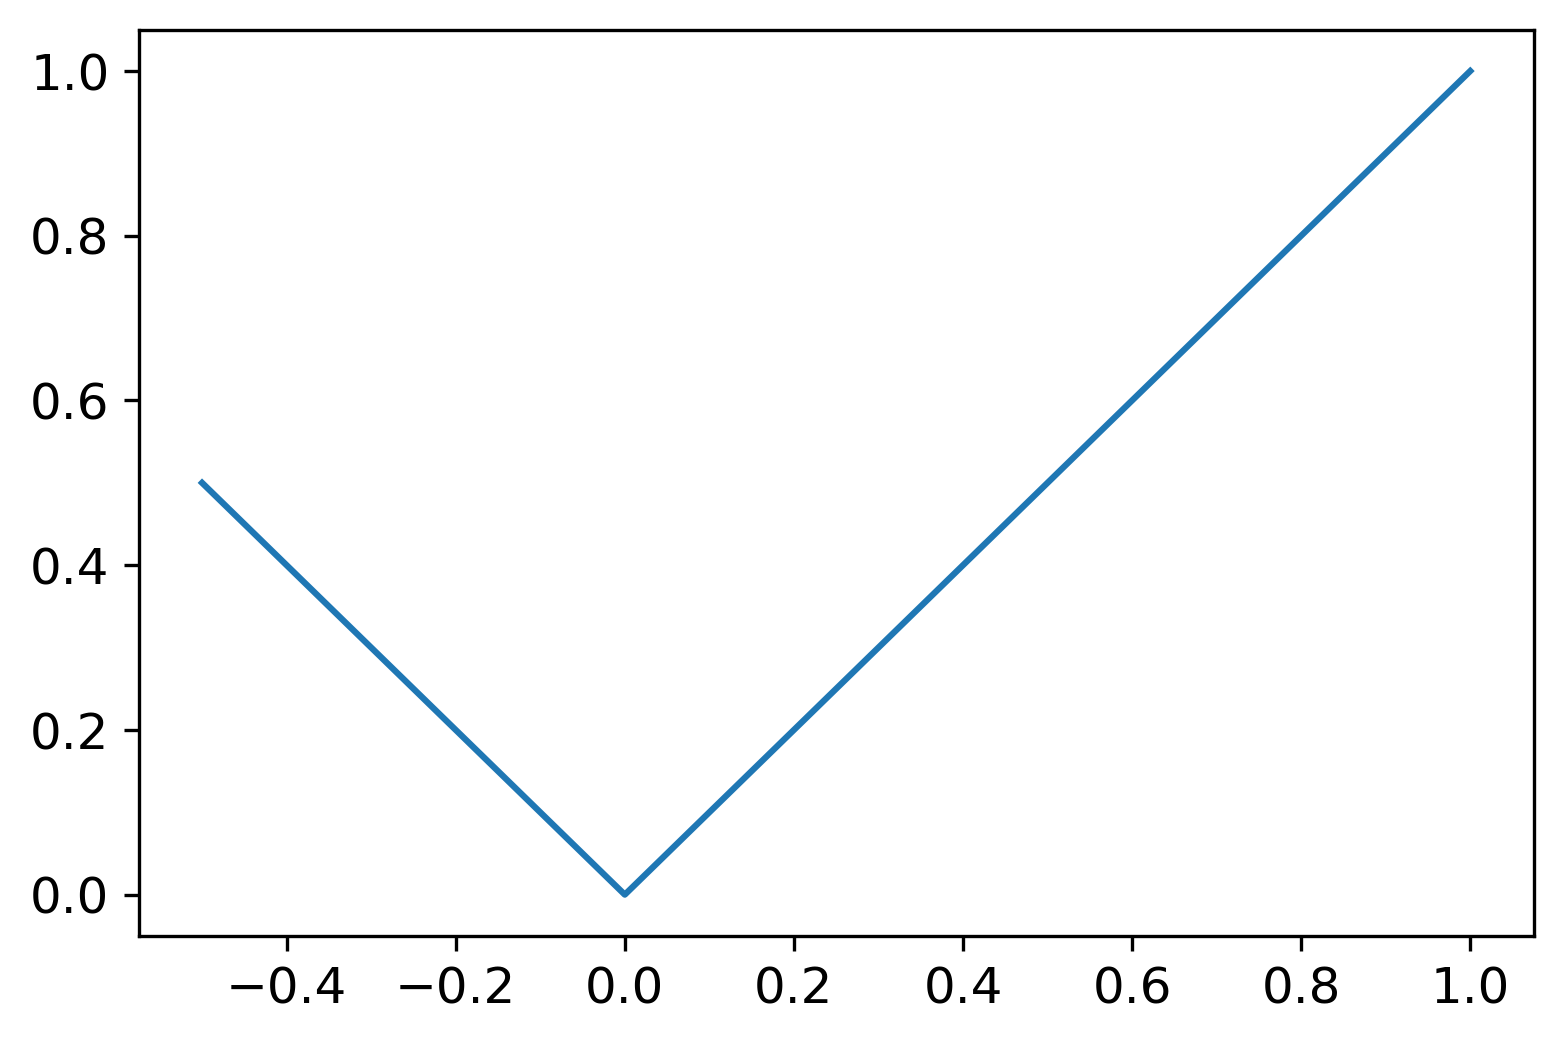
\includegraphics[width=3.5in]{./cap_ag/dados/fig_absx/fig.png}
  \caption{Gráfico referente ao Exemplo~\ref{cap_ag_sec_graf:ex:absx}.}
  \label{cap_ag_sec_graf:fig:absx}
\end{figure}


\begin{ex}\label{cap_ag_sec_graf:ex:absx}
  Consideramos a função
  \begin{equation}
    f(x) = |x|, ~-\frac{1}{2}\leq x < 1.
  \end{equation}
  A Figura~\ref{cap_ag_sec_graf:fig:absx}, mostra o gráfico de $f$ plotado com o código abaixo.
  
\begin{lstlisting}
import matplotlib.pyplot as plt

# figure
fig = plt.figure()
# axes
ax = fig.add_subplot()
# plot
ax.plot([-0.5, 0, 1],
        [0.5, 0, 1])
# display
plt.show()
\end{lstlisting}

\end{ex}

No caso de curvas, podemos usamos um número adequado de pontos de forma que os segmentos de linhas fiquem imperceptíveis a olho nu.

\begin{ex}\label{cap_ag_sec_graf:ex:fun}
  Consideramos a função
  \begin{equation}
    f(x) = \left\{
      \begin{array}{ll}
        -(x+1)^2-2 &, ~-2\leq x < -\frac{1}{2},\\
        |x| &, ~-\frac{1}{2}\leq x < 1,\\
        (x-2)^3 + 2, &, ~1\leq x < 3.
      \end{array}
    \right.
  \end{equation}
  A Figura~\ref{cap_ag_sec_graf:fig:fun}, mostra o gráfico de $f$ plotado com o código abaixo.

  \begin{figure}[H]
    \centering
    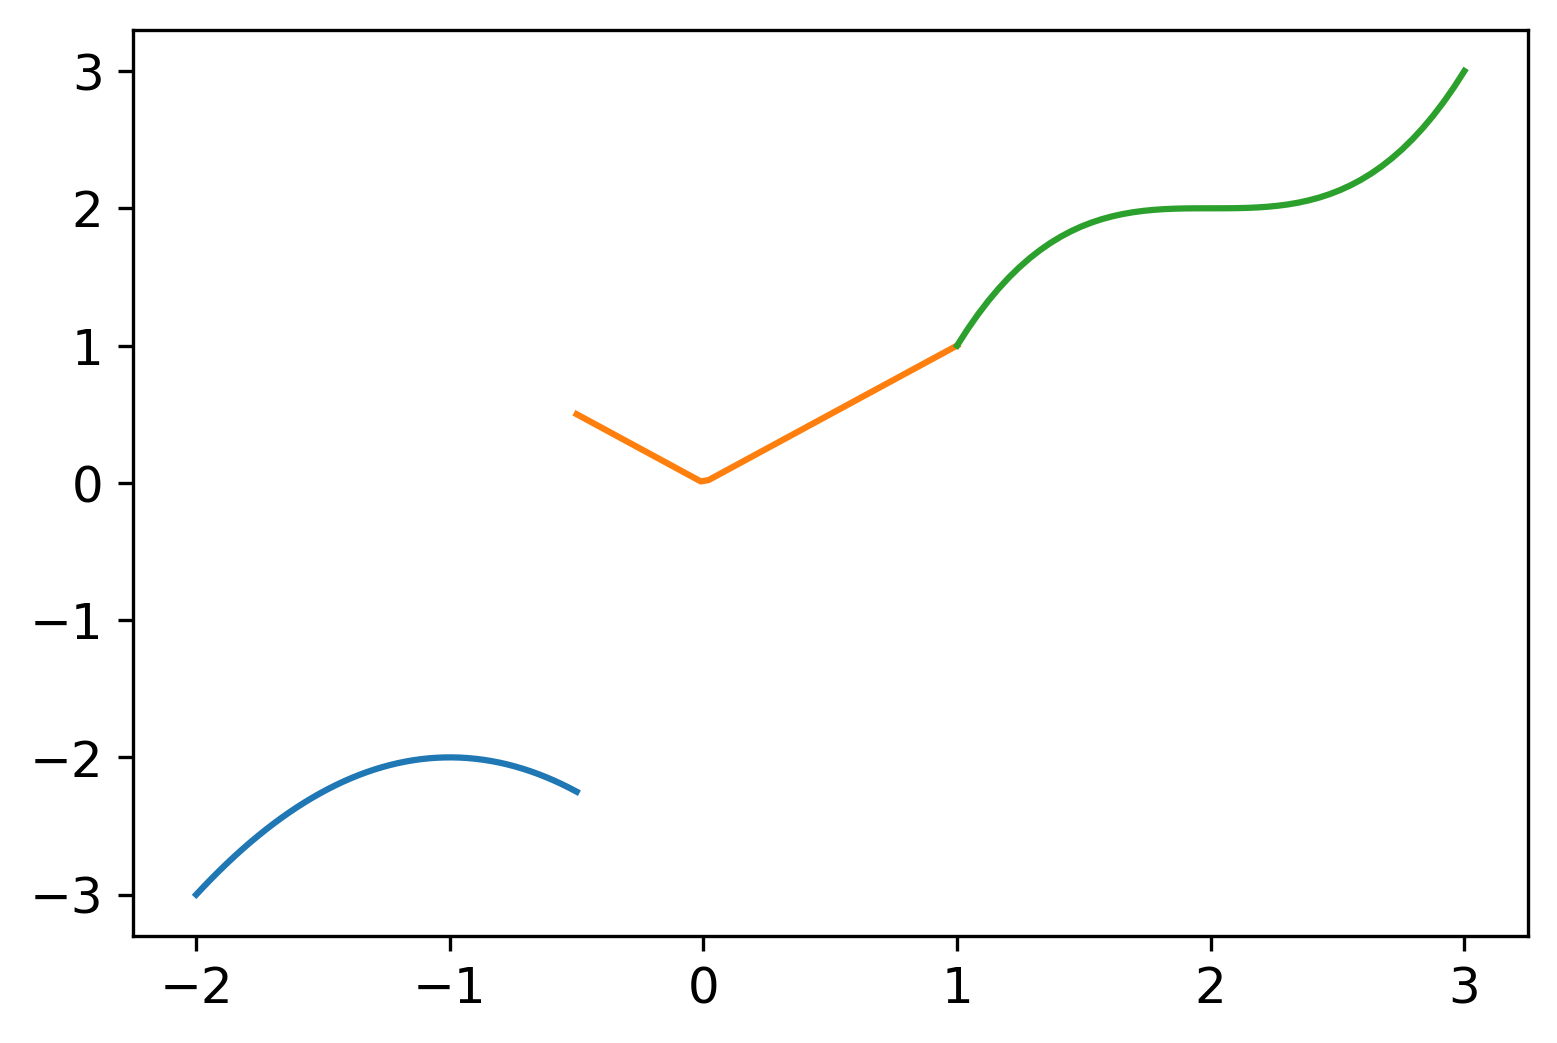
\includegraphics[width=3.5in]{./cap_ag/dados/fig_fun/fig.png}
    \caption{Gráfico referente ao Exemplo~\ref{cap_ag_sec_graf:ex:fun}.}
    \label{cap_ag_sec_graf:fig:fun}
  \end{figure}  

\begin{lstlisting}
import matplotlib as mpl
import matplotlib.pyplot as plt
import numpy as np

# figure
fig = plt.figure()
# axis
ax = fig.add_subplot()
# -2 <= x < -0.5
x = np.linspace(-2, -0.5)
ax.plot(x, -(x+1)**2-2)
# -0.5 <= x < 1
x = np.linspace(-0.5, 1)
ax.plot(x, np.fabs(x))
# 1 <= x < 3
x = np.linspace(1, 3)
ax.plot(x, (x-2)**3+2)
# display
plt.show()
\end{lstlisting}

\end{ex}

\subsection{Eixos}

No {\PYTHONmatplotlib}, os eixos\endnote{Não confundir com {\PYTHONmatplotlibDOTaxesDOTAxes}, um objeto que contém todos os elementos de um gráfico.} de um gráfico são objetos da classe {\PYTHONmatplotlibDOTaxisDOTAxis}.

\begin{ex}\label{cap_ag_sec_graf:ex:axis}
  Com o código abaixo, produzimos a Figura~\ref{cap_ag_sec_graf:fig:eixos}, a qual contém o gráfico da função do Exemplo~\ref{cap_ag_sec_graf:fig:fun} com os eixos editados.

  \begin{figure}[H]
    \centering
    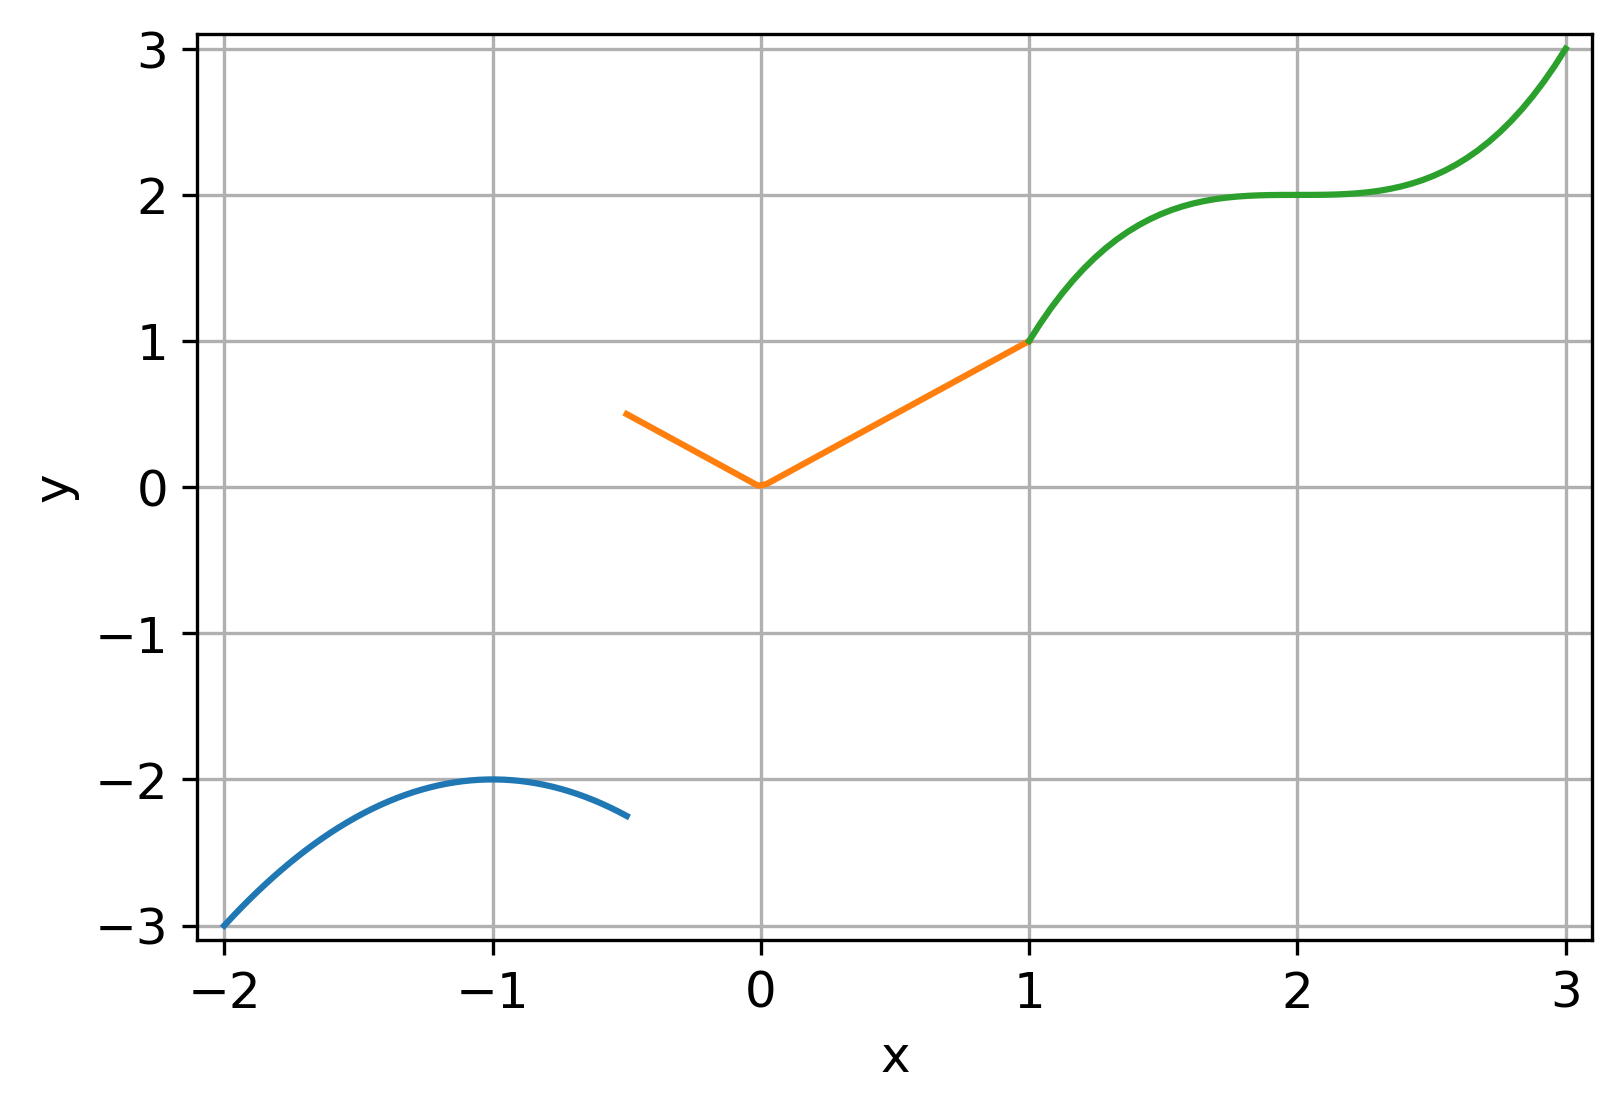
\includegraphics[width=3.5in]{./cap_ag/dados/fig_eixos/fig.png}
    \caption{Gráfico referente ao Exemplo~\ref{cap_ag_sec_graf:ex:axis}.}
    \label{cap_ag_sec_graf:fig:eixos}
  \end{figure}  

\begin{lstlisting}
import matplotlib as mpl
import matplotlib.pyplot as plt
import numpy as np

# figure
fig = plt.figure()
# axis
ax = fig.add_subplot()
# -2 <= x < -0.5
x = np.linspace(-2, -0.5)
ax.plot(x, -(x+1)**2-2)
# -0.5 <= x < 1
x = np.linspace(-0.5, 1)
ax.plot(x, np.fabs(x))
# 1 <= x < 3
x = np.linspace(1, 3)
ax.plot(x, (x-2)**3+2)
# eixo-x
ax.set_xlim((-2.1, 3.1))
ax.set_xticks([-2, -1, 0, 1, 2, 3])
ax.set_xlabel('x')
#eixo-y
ax.set_ylim((-3.1, 3.1))
ax.set_yticks([-3, -2, -1, 0, 1, 2, 3])
ax.set_ylabel('y')
# grid
ax.grid()
# display
plt.savefig('fig.png', bbox_inches='tight')
plt.savefig('fig.pdf', bbox_inches='tight')
plt.show()
\end{lstlisting}

\end{ex}

\subsection{Elementos Gráficos}

No {\PYTHONmatplotlib}, os elementos gráficos (basicamente tudo o que é visível, pontos, linhas, eixos, etc.) são objetos da classe {\PYTHONmatplotlibDOTartistDOTArtist}.

\begin{ex}\label{cap_ag_sec_graf:ex:elgraf}
  Com o código abaixo, produzimos a Figura~\ref{cap_ag_sec_graf:fig:elgraf}, a qual contém o gráfico da função do Exemplo~\ref{cap_ag_sec_graf:fig:elgraf} com os eixos editados.

  \begin{figure}[H]
    \centering
    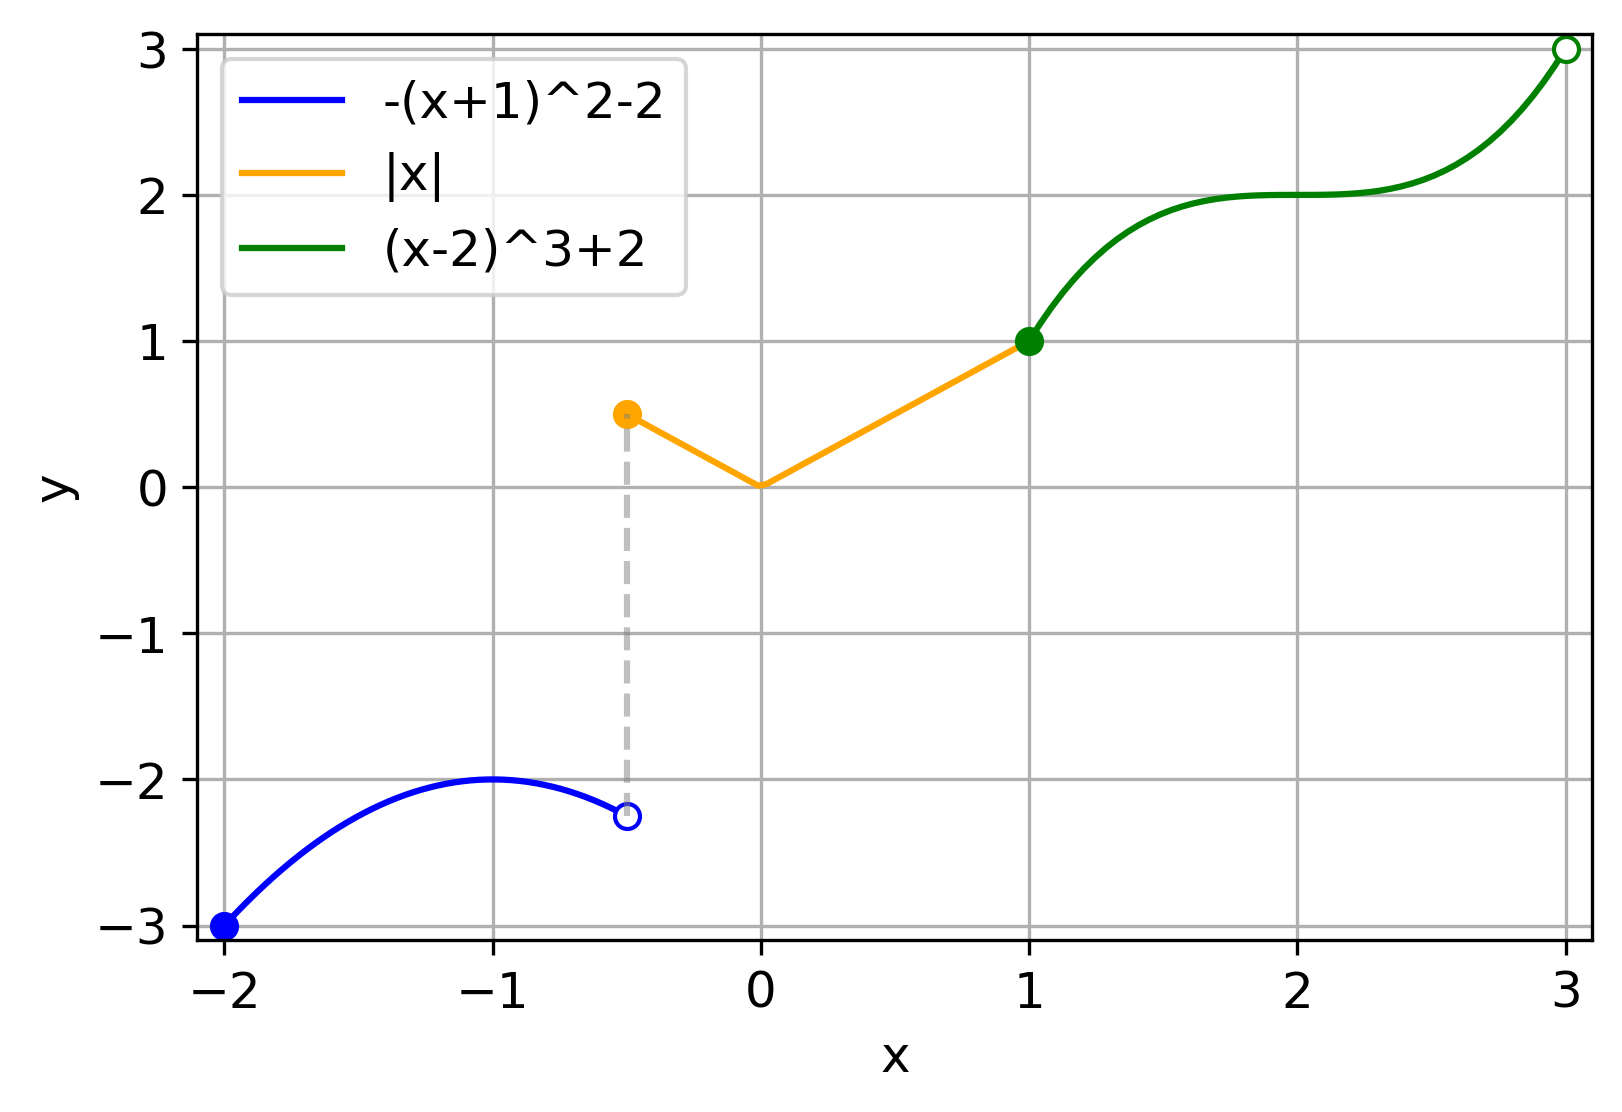
\includegraphics[width=3.5in]{./cap_ag/dados/fig_elgraf/fig.png}
    \caption{Gráfico referente ao Exemplo~\ref{cap_ag_sec_graf:ex:elgraf}.}
    \label{cap_ag_sec_graf:fig:elgraf}
  \end{figure}
  
\begin{lstlisting}
import matplotlib as mpl
import matplotlib.pyplot as plt
import numpy as np

# figure
fig = plt.figure()
# axis
ax = fig.add_subplot()

# -2 <= x < -0.5
x = np.linspace(-2, -0.5)
f1 = lambda x: -(x+1)**2-2
ax.plot(x, f1(x), color='blue',
        label='-(x+1)^2-2')
ax.plot([-2.], f1(-2.), linestyle='', marker='o',
        color='blue')
ax.plot([-0.5], f1(-0.5), ls='', marker='o',
        markerfacecolor='white', markeredgecolor='blue')

# -0.5 <= x < 1
x = np.linspace(-0.5, 1)
f2 = lambda x: np.fabs(x)
ax.plot(x, f2(x), color='orange', label='|x|')
ax.plot([-0.5], [f2(-0.5)], ls='', marker='o',
        color='orange')

ax.plot([-0.5, -0.5], [f1(-0.5), f2(-0.5)],
        ls = '--', color='gray', alpha=0.5)

# 1 <= x < 3
x = np.linspace(1, 3)
f3 = lambda x: (x-2)**3+2
ax.plot(x, f3(x), color='green',
        label='(x-2)^3+2')
ax.plot([1.], [f3(1.)], ls='', marker='o',
        color='green')
ax.plot([3.], [f3(3.)], ls='', marker='o',
        mfc='white', mec='green')

# eixo-x
ax.set_xlim((-2.1, 3.1))
ax.set_xticks([-2, -1, 0, 1, 2, 3])
ax.set_xlabel('x')
# eixo-y
ax.set_ylim((-3.1, 3.1))
ax.set_yticks([-3, -2, -1, 0, 1, 2, 3])
ax.set_ylabel('y')
# grid
ax.grid()
ax.legend()
# display
plt.savefig('fig.png', bbox_inches='tight')
plt.savefig('fig.pdf', bbox_inches='tight')
plt.show()
\end{lstlisting}

\end{ex}

\subsection{Textos e Anotações}

O comando {\PYTHONmatplotlibDOTaxesDOTAxesDOTtext} permite adicionar elementos \texttt{string} a um {\PYTHONmatplotlibDOTaxesDOTAxes}. Anotações, consistem em um apontamento, e podem ser adicionadas com o comando {\PYTHONmatplotlibDOTaxesDOTAxesDOTannotate}. Elementos texto suportam {\LaTeX} usando-se o marcador de texto \lstinline!$!.%$

\begin{ex}\label{cap_ag_sec_graf:ex:texto}
  Com o código abaixo, produzimos a Figura~\ref{cap_ag_sec_graf:fig:texto}, a qual contém o gráfico da função do Exemplo~\ref{cap_ag_sec_graf:fig:texto} com os eixos editados.

  \begin{figure}[H]
    \centering
    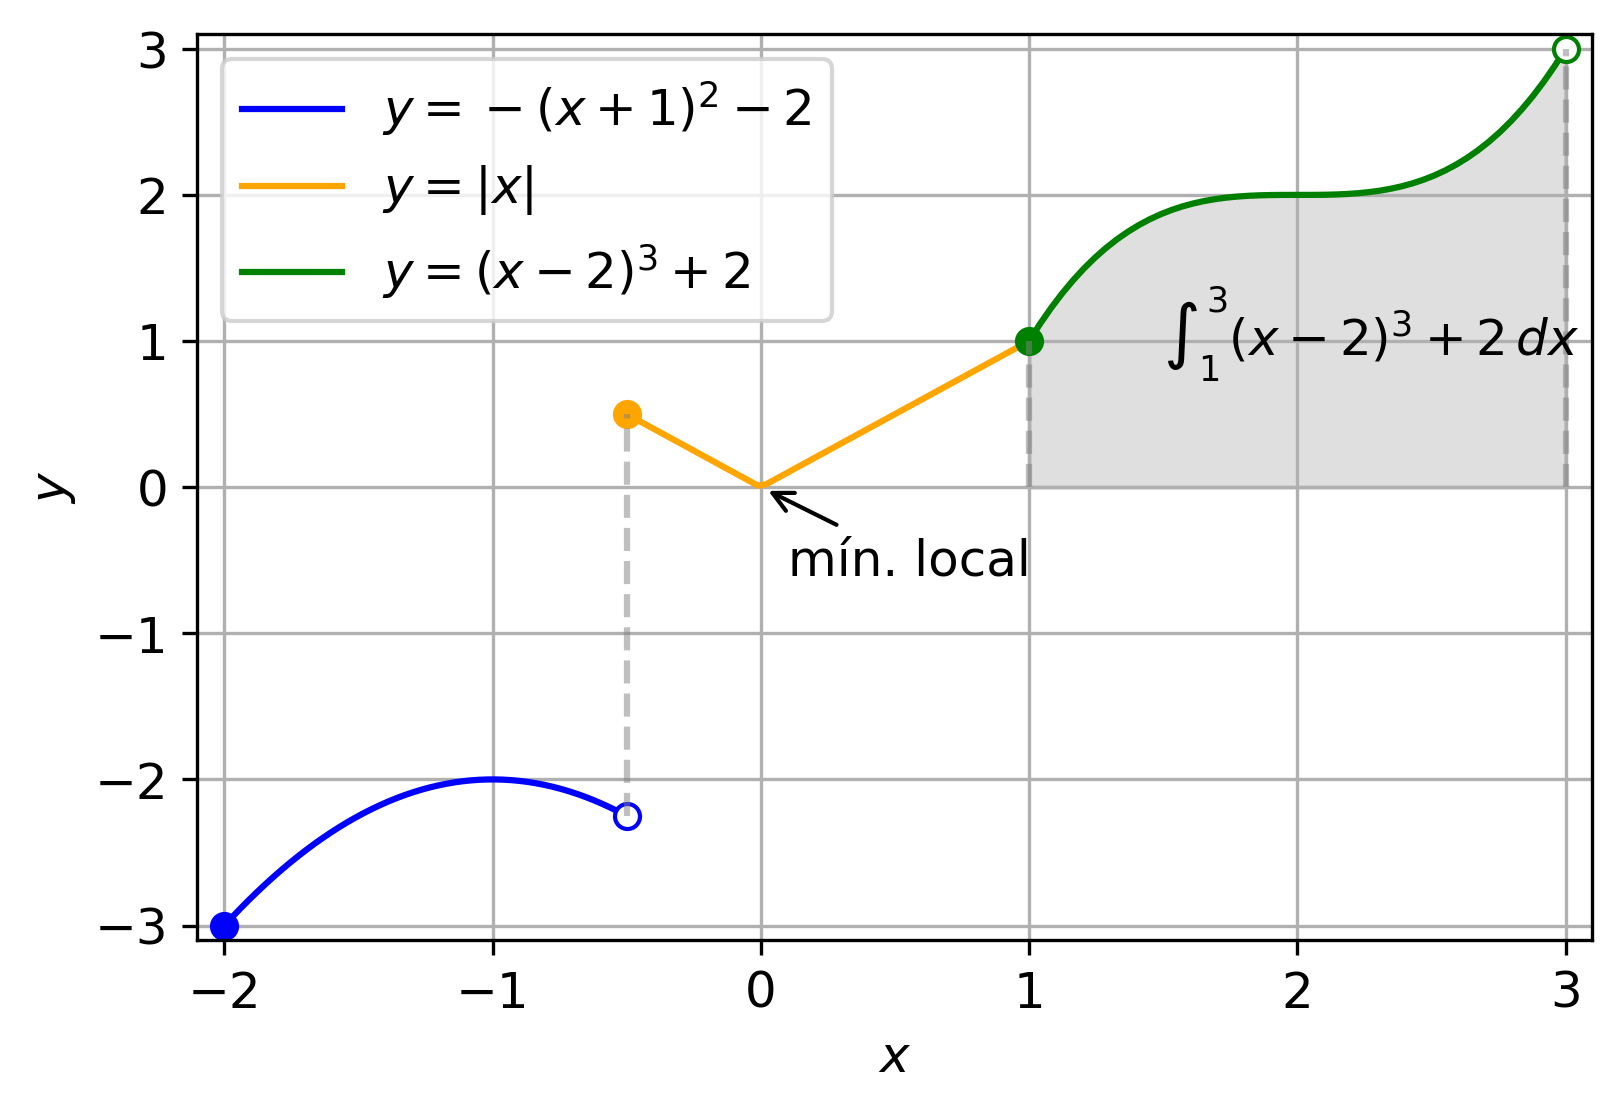
\includegraphics[width=3.5in]{./cap_ag/dados/fig_texto/fig.png}
    \caption{Gráfico referente ao Exemplo~\ref{cap_ag_sec_graf:ex:texto}.}
    \label{cap_ag_sec_graf:fig:texto}
  \end{figure}
  
\begin{lstlisting}
import matplotlib as mpl
import matplotlib.pyplot as plt
import numpy as np

# figure
fig = plt.figure()
# axis
ax = fig.add_subplot()

# -2 <= x < -0.5
x = np.linspace(-2, -0.5)
f1 = lambda x: -(x+1)**2-2
ax.plot(x, f1(x), color='blue',
        label='$y=-(x+1)^2-2$')
ax.plot([-2.], f1(-2.), linestyle='', marker='o',
        color='blue')
ax.plot([-0.5], f1(-0.5), ls='', marker='o',
        markerfacecolor='white', markeredgecolor='blue')

# -0.5 <= x < 1
x = np.linspace(-0.5, 1)
f2 = lambda x: np.fabs(x)
ax.plot(x, f2(x), color='orange', label='$y=|x|$')
ax.plot([-0.5], [f2(-0.5)], ls='', marker='o',
        color='orange')

ax.plot([-0.5, -0.5], [f1(-0.5), f2(-0.5)],
        ls = '--', color='gray', alpha=0.5)
# anotação
ax.annotate('mín. local', xy=(0,0), xytext=(0.1,-0.6),
            arrowprops={'arrowstyle':'->'})

# 1 <= x < 3
x = np.linspace(1, 3)
f3 = lambda x: (x-2)**3+2
ax.plot(x, f3(x), color='green',
        label='$y=(x-2)^3+2$')
ax.plot([1.], [f3(1.)], ls='', marker='o',
        color='green')
ax.plot([3.], [f3(3.)], ls='', marker='o',
        mfc='white', mec='green')

# hachurando
ax.fill_between(x, f3(x), color='gray', alpha=0.25)
ax.plot([1., 1.], [0., f3(1.)],
        ls='--', color='gray', alpha=0.5)
ax.plot([3., 3.], [0., f3(3.)],
        ls='--', color='gray', alpha=0.5)
# texto
ax.text(1.5, 0.9, '$\\int_{1}^3 (x-2)^3+2\,dx$')

# eixo-x
ax.set_xlim((-2.1, 3.1))
ax.set_xticks([-2, -1, 0, 1, 2, 3])
ax.set_xlabel('$x$')
# eixo-y
ax.set_ylim((-3.1, 3.1))
ax.set_yticks([-3, -2, -1, 0, 1, 2, 3])
ax.set_ylabel('$y$')
# grid
ax.grid()
ax.legend()
# display
plt.savefig('fig.png', bbox_inches='tight')
plt.savefig('fig.pdf', bbox_inches='tight')
plt.show()
\end{lstlisting}

\end{ex}

\subsection{Exercícios}

% exercícios de compreensão

\begin{exer}
  Complete as lacunas.
  \begin{enumerate}[a)]
    % a)
    \item Gráficos são colocados em um \textit{container} \underline{\phantom{\PYTHONmatplotlibDOTfigureDOTFigure}}.
    % b)
    \item Um {\PYTHONmatplotlibDOTfigureDOTFigure} pode conter um ou mais {\PYTHONmatplotlibDOTaxesDOTAxes}.
    % c)
    \item Os eixos (abscissas, ordenadas, etc.) de um gráficos são objetos da classe \underline{\phantom{\PYTHONmatplotlibDOTaxisDOTAxis}}.
    % d)
    \item Os elementos gráficos como pontos, linhas, eixos, etc. são objetos da classe \underline{\phantom{\PYTHONmatplotlibDOTartistDOTArtist}}.
  \end{enumerate}
\end{exer}
\begin{resp}
  a) {\PYTHONmatplotlibDOTfigureDOTFigure}; b) {\PYTHONmatplotlibDOTaxesDOTAxes}; c) {\PYTHONmatplotlibDOTaxisDOTAxis}; d) {\PYTHONmatplotlibDOTartistDOTArtist}
\end{resp}

% exercícios de programação

\begin{exer}
  Use o {\matplotlib} para produzir um gráfico para as seguintes funções:
  \begin{enumerate}[a)]
  \item $\displaystyle f(x) = x^2$, $-2 \leq x \leq 2$.
  \item $\displaystyle g(x) = 2x^3+2$, $-3 \leq x \leq 0$.
  \item $\displaystyle h(x) = \sen(x)$, $-\pi \leq x \leq \pi$.
  \end{enumerate}
\end{exer}

\begin{exer}
  Use o {\matplotlib} para plotar o gráfico da função sigmoid
  \begin{equation}
    f(x) = \frac{1}{1 + e^{-x}}.
  \end{equation}
  Na mesma área gráfica, plote retas tracejadas identificando suas assíntotas horizontais.
\end{exer}
\begin{resp}
  Dica: $y = 0$ e $y=1$ são assíntotas horizontais da função sigmoid.
\end{resp}

\begin{exer}
  Use o {\matplotlib} para plotar o gráfico de $f(x) = 1/x$, $-2 \leq x \leq 2$. Na mesma área gráfica, plote uma reta tracejada identificando a assíntota vertical de $f$.
\end{exer}
\begin{resp}
  Dica: $x = 0$ é assíntota vertical de $f$.
\end{resp}

\begin{exer}
  Use o {\matplotlib} para produzir um gráfico para a seguinte função definida por partes
  \begin{equation}
    f(x) = \left\{
      \begin{array}{ll}
        \cos(x) &, -\pi < x \leq 0,\\
        1-x^2 &, 0 < x \leq 2.
      \end{array}
    \right.
  \end{equation}
  Use de marcadores para identificar os pontos extremos de cada parte da função. Também, adicione o \textit{label} de cada eixo e uma legenda para identificar cada parte da função.
\end{exer}

\begin{exer}
  Em uma mesma área gráfica, plote as curvas $y = x + 1$ e $y = x^2$, e marque seus pontos de interseção. Para cada um destes pontos, inclua a anotação ``pto. de interseção''.
\end{exer}

\begin{exer}
  No gráfico da função sigmoid
  \begin{equation}
    f(x) = \frac{1}{1 + e^{-x}}
  \end{equation}
  hachure (pinte) a região que corresponde a área associada a integral definida
  \begin{equation}
    \int_1^3 f(x)\,dx.
  \end{equation}
\end{exer}
\begin{resp}
  Dica: use a função {\PYTHONmatplotlibDOTaxesDOTAxesDOTfillBetween}.
\end{resp}

\begin{ex}
  Em uma mesma área gráfica, plote a área entre as curvas $y = x + 1$ e $y = x^2$, $x=-1$ e $x=2$.
\end{ex}

\ifisbook
\subsubsection{Respostas}
\shipoutAnswer
\fi

\chapter{Orientação a Objetos}\label{cap_poo}

\hl{\emph{Programação Orientação a Objetos} (POO) é um paradigma de programação baseado no conceito de classes de objetos. A \emph{classe} define os atributos (propriedades e métodos) de seus \emph{objetos}}. Todos os objetos de uma classe têm os mesmos atributos, mas são independentes um dos outros, sendo que cada um é uma instância própria da classe contendo seus próprios valores de seus atributos.

\section{Classe e Objeto}\label{cap_ob_sec_class}

\hl{Uma \emph{classe} é uma forma de estrutura que permite a alocação conjunta de dados e funções}. Em {\python}, a sintaxe de definição de uma classe é

\begin{lstlisting}
class NomeDaClasse:
  <bloco-0>
  <bloco-1>
  ...
  <bloco-2>
\end{lstlisting}

Usualmente, \hl{os blocos de programação consistem de definições de funções (métodos)}. Por exemplo,

\begin{lstlisting}
class MinhaClasse:
  def digaOla(self):
    print('Olá, Mundo!')

obj = MinhaClasse()
obj.digaOla()
\end{lstlisting}

Neste código, temos a definição da classe \lstinline+MinhaClasse+ (linhas 1-3). Esta classe contém o método \lstinline+MinhaClasse.digaOla()+ (linhas 2-3). Obrigatoriamente, \hl{na definição de um método de uma classe deve conter o primeiro parâmetro \texttt{self}}. Um objeto desta classe\endnote{Uma nova instância da classe.} e identificado por \lstinline+obj+ é alocado na linha 5. Na linha 6, este objeto chama seu método \lstinline+obj.digaOla()+.

O método especial {\PYTHONobjectDOTinit} é executado na construção de cada nova instância da classe (objeto da classe). Por exemplo,

\begin{lstlisting}
class Brasileira:
  pais = 'Brasil'
  def __init__(self, nome):
    self.nome = nome
      
  def digaOla(self):
    print('\nOlá!')
    print(f'Eu me chamo {self.nome}.')
    print(f'Sou do {self.pais}. :)')

x = Brasileira('Fulane')
x.digaOla()
y = Brasileira('Beltrane')
y.digaOla()
\end{lstlisting}

Aqui, o atributo \lstinline+Brasileira.pais+ é compartilhada entre todas as instâncias da classe (objetos), enquanto que \lstinline+Brasileira.nome+ é um atributo de cada objeto. O método {\PYTHONobjectDOTinit} (linhas 3-4) é executada no momento da criação de cada nova instância (linhas 11 e 13).

\begin{ex}\label{cap_oo_sec_class:ex:triangulo}
  No seguinte código, começamos a definição de uma classe para a manipulação de triângulos.

\begin{lstlisting}[caption=classTriangulo.py, label=cap_poo_sec_class:cod:classTriangulo]
import matplotlib.pyplot as plt

class Triangulo:
  '''
  Classe Triangulo ABC.
  '''
  num_lados = 3
  def __init__(self, A, B, C):
    # vértices
    self.A = A
    self.B = B
    self.C = C

  def plot(self):
    fig = plt.figure()
    ax = fig.add_subplot()
    # lados
    ax.plot([self.A[0], self.B[0]],
            [self.A[1], self.B[1]], marker='o', color='blue')
    ax.text((self.A[0]+self.B[0])/2,
            (self.A[1]+self.B[1])/2, 'c')
    ax.plot([self.B[0], self.C[0]],
            [self.B[1], self.C[1]], marker='o', color='blue')
    ax.text((self.B[0]+self.C[0])/2,
            (self.B[1]+self.C[1])/2, 'a')
    ax.plot([self.C[0], self.A[0]],
            [self.C[1], self.A[1]], marker='o', color='blue')
    ax.text((self.A[0]+self.C[0])/2,
            (self.A[1]+self.C[1])/2, 'b')
    # vertices
    ax.text(self.A[0], self.A[1], 'A')
    ax.text(self.B[0], self.B[1], 'B')
    ax.text(self.C[0], self.C[1], 'C')
    ax.grid()
    plt.show()

tria = Triangulo((0., 0.),
                (2., 0.),
                (1., 1.))
tria.plot()
\end{lstlisting}

\end{ex}

\subsection{Exercícios}

\begin{exer}
  Considere o Código~\ref{cap_poo_sec_class:cod:classTriangulo}. Adicione o método \lstinline+calcLados()+, que computa e aloca o comprimento de cada lado do triângulo.
\end{exer}
\begin{resp}

\begin{lstlisting}
import numpy as np
import matplotlib.pyplot as plt

class Triangulo:
  '''
  Classe Triangulo ABC.
  '''
  num_lados = 3
  def __init__(self, A, B, C):
    # vértices
    self.A = A
    self.B = B
    self.C = C
    # lados
    self.a = 0.
    self.b = 0.
    self.c = 0.

  def calcLados(self):
    self.a = np.sqrt((self.B[0]-self.C[0])**2\
                      + (self.B[1]-self.C[1])**2)
    self.b = np.sqrt((self.A[0]-self.C[0])**2\
                      + (self.A[1]-self.C[1])**2)
    self.c = np.sqrt((self.A[0]-self.B[0])**2\
                      + (self.A[1]-self.B[1])**2)
\end{lstlisting}

\end{resp}

\begin{exer}
  Considere o Código~\ref{cap_poo_sec_class:cod:classTriangulo}. Adicione o método \lstinline+calcPerimetro()+, que computa e retorna o valor do perímetro do triângulo.
\end{exer}
\begin{resp}

\begin{lstlisting}
import numpy as np
import matplotlib.pyplot as plt

class Triangulo:

  ...

  def perimetro(self):
    return self.a + self.b + self.c

  ...
\end{lstlisting}

\end{resp}

\begin{exer}
  Considere o Código~\ref{cap_poo_sec_class:cod:classTriangulo}. Adicione o método \lstinline+calcAngulos()+, que computa e aloca os ângulos do triângulo.
\end{exer}
\begin{resp}
  Dica: use a \href{https://pt.wikipedia.org/wiki/Lei_dos_cossenos}{Lei dos Cossenos}.
\end{resp}

\begin{exer}
  Considere o Código~\ref{cap_poo_sec_class:cod:classTriangulo}. Adicione o método \lstinline+area()+, que computa a área do triângulo.
\end{exer}
\begin{resp}
  Dica: use o \href{https://pt.wikipedia.org/wiki/Teorema_de_Her%C3%A3o}{Teorema de Herão}.
\end{resp}

\begin{exer}
  Similar a classe \lstinline+Triangulo+ (Código~\ref{cap_poo_sec_class:cod:classTriangulo}), implemente uma nova classe \lstinline+Quadrilateros+ com as seguintes propriedades e métodos de quadriláteros $ABCD$:
  \begin{enumerate}[a)]
  \item vértices (\lstinline+tuples+).
  \item lados (\lstinline+floats+).
  \item cálculo do perímetro (método).
  \item cálculo da área (método).
  \item visualização gráfica (método \textit+plot+).
  \end{enumerate}
\end{exer}

\begin{exer}
  Implemente uma classe para a manipulação de polinômios de segundo grau. A classe deve conter as seguintes propriedades e métodos:
  \begin{enumerate}[a)]
  \item coeficientes (\lstinline+floats+).
  \item cálculo do ponto de interseção com o eixo y (método).
  \item cálculo do vértice da parábola associada ao polinômio (método).
  \item cálculo das raízes do polinômio (método).
  \item plotagem do gráfico do polinômio (método).
  \end{enumerate}
\end{exer}
\begin{resp}
  Dica: utilize a notação $p(x) = ax^2 + bx + c$.
\end{resp}

\ifisbook
\subsubsection{Respostas}
\shipoutAnswer
\fi

  

\section{Herança}\label{cap_oo_sec_her}

\hl{Na programação orientada-a-objetos, \emph{herança} consiste na definição de uma classe derivada a partir de uma dada classe base}. A sintaxe de definição de uma classe derivada é

\begin{lstlisting}
class ClasseDerivada(ClasseBase):
  bloco-0
  bloco-1
  ...
  bloco-n
\end{lstlisting}

\hl{A classe derivada herda todos os atributos da classe base}. Por exemplo, consideramos o seguinte código

\ifisbook
\newpage
\fi
\begin{lstlisting}
class ClasseBase:
  def __init__(self, nome):
    self.nome = nome
      
  def digaOi(self):
    print(f'{self.nome}: Oi!')

class ClasseDerivada(ClasseBase):
  def digaTchau(self):
    print(f'{self.nome}: Tchau!')

obj = ClasseDerivada('Fulane')
obj.digaOi()
obj.digaTchau()
\end{lstlisting}

Nas linhas 1-6, a classe base é definida contendo dois métodos: {\PYTHONobjectDOTinit} chamado na criação de um objeto da classe (uma instância) e, \lstinline+self.digaOi()+ que imprime uma saudação. A classe derivada é definida nas linhas 8-10, ela herda os atributos da classe base e contém um novo método \lstinline+self.digaTchau()+, que imprime uma mensagem de despedida.

A criação de uma instância (objeto) de uma classe derivada é feita da mesma forma que de uma classe base. \hl{A referência a um atributo do objeto é, primeiramente, buscada na classe derivada e, se não encontrada, é buscada na classe base}. Este regra aplica-se recursivamente se a classe base também é derivada de outra classe. \hl{Isso permite que uma classe derivada sobreponha atributos de sua classe base}.

\begin{obs}[\hl{\texttt{super()}}]
O método {\PYTHONsuper} retorna um objeto \textit{proxy} da classe base, que acessa os atributos desta.
\end{obs}

\begin{ex}
  Vamos criar uma classe para manipular triângulo isósceles. Para tanto, vamos derivá-la a partir da classe \lstinline+Triangulo+ definida no Exemplo~\ref{cap_oo_sec_class:ex:triangulo}. Vamos assumir que os triângulos isósceles têm vértices $\Delta ABC$ com lados $b = AC$ e $a = BC$ de mesmo tamanho.

\begin{lstlisting}[caption=classTrianguloIsosceles.py, label=cap_oo_sec_her:cod:classTrianguloIsosceles]
import numpy as np
import matplotlib.pyplot as plt

class Triangulo:
  '''
  Classe Triangulo ABC.
  '''
  num_lados = 3
  def __init__(self, A, B, C):
    # vértices
    self.A = A
    self.B = B
    self.C = C

  def plot(self):
    fig = plt.figure()
    ax = fig.add_subplot()
    # lados
    ax.plot([self.A[0], self.B[0]],
            [self.A[1], self.B[1]], marker='o', color='blue')
    ax.text((self.A[0]+self.B[0])/2,
            (self.A[1]+self.B[1])/2, 'c')
    ax.plot([self.B[0], self.C[0]],
            [self.B[1], self.C[1]], marker='o', color='blue')
    ax.text((self.B[0]+self.C[0])/2,
            (self.B[1]+self.C[1])/2, 'a')
    ax.plot([self.C[0], self.A[0]],
            [self.C[1], self.A[1]], marker='o', color='blue')
    ax.text((self.A[0]+self.C[0])/2,
            (self.A[1]+self.C[1])/2, 'b')
    # vertices
    ax.text(self.A[0], self.A[1], 'A')
    ax.text(self.B[0], self.B[1], 'B')
    ax.text(self.C[0], self.C[1], 'C')
    ax.grid()
    plt.show()


class TrianguloIsosceles(Triangulo):
  def __init__(self,A,B,C):
    # vertices
    super().__init__(A,B,C)
    # lados
    self.a = self.b = self.c = 0.

  def calcLados(self):
    self.a = np.sqrt((self.B[0] - self.C[0])**2\
                      + (self.B[1] - self.C[1])**2)
    self.b = np.sqrt((self.A[0] - self.C[0])**2\
                      + (self.A[1] - self.C[1])**2)
    self.c = np.sqrt((self.B[0] - self.A[0])**2\
                      + (self.B[1] - self.A[1])**2)
    assert(self.a == self.b)

tria = TrianguloIsosceles((1,0),
                          (3,0),
                          (2,1))
tria.plot()
tria.calcLados()
\end{lstlisting}

\end{ex}

\begin{obs}[\hl{Herança Múltipla}]
  {\python} suporta a herança múltipla de classes. A sintaxe é

\begin{lstlisting}
class ClasseDerivada(Base1, Base2, ..., BraseN):
  bloco-0
  bloco-1
  ...
  bloco-m
\end{lstlisting}
  
Quando um objeto da classe derivada faz uma referência a um atributo, este é procurado de forma sequencial (e recursiva, caso uma das classe bases seja também uma classe derivada) começando por essa e, caso não encontrado, buscando-se nas classes \lstinline+Base1+, \lstinline+Base2+, ..., \lstinline+BaseN+.
\end{obs}

\subsection{Exercícios}

\begin{exer}
  No Código~\ref{cap_oo_sec_her:cod:classTrianguloIsosceles}, adicione à classe \lstinline+Triangulo+ o método \lstinline+Triangulo.perimetro()+ que computa, aloca e retorna o valor do perímetro do triângulo. Então, sobreponha o método à classe \lstinline+TrianguloIsosceles+. Teste seu código para diferentes triângulos.
\end{exer}
\begin{resp}

\begin{lstlisting}
class Triangulo:
  def __init(self,A,B,C)__:
    ...
    self.p = 0.
    ...
  ...
  def perimetro(self):
    self.p = self.a\
            + self.b\
            + self.c
    return self.p
  ...

class TrianguloIsosceles(Triangulo):
  ...
  def perimetro(self):
    self.p = 2*self.a + self.c
    return self.p
  ...
\end{lstlisting}

\end{resp}

\begin{exer}\label{cap_oo_sec_her:exer:retangulo}
  Implemente uma classe \lstinline+Retangulo(largura, altura)+ para a manipulação de retângulos de \lstinline+largura+ e \lstinline+altura+ dadas. Equipe sua classe com métodos para o cálculo do perímetro, da diagonal e da área de retângulo. Então, implemente a classe derivada \lstinline+Quadrado(lado)+ para a manipulação de quadrados de \lstinline+lado+ dado. Teste sua implementação para diferentes retângulos e quadrados.
\end{exer}
\begin{resp}

\begin{lstlisting}
import math as m

class Retangulo:
  def __init__(self, largura, altura):
    self.largura = largura
    self.altura = altura

  def perimetro(self):
    return self.largura\
            + self.altura

  def diagonal(self):
    return m.sqrt(self.largura**2\
                  + self.altura**2)

  def area(self):
    return self.largura\
            * self.altura

class Quadrado(Retangulo):
  def __init__(self,lado):
    super().__init__(lado,lado)
\end{lstlisting}

\end{resp}

\begin{exer}
  Refaça o Exercício~\ref{cap_oo_sec_her:exer:retangulo} sobrepondo os métodos do cálculo do perímetro, da diagonal e da área para quadrados.
\end{exer}
\begin{resp}
  Dica: para um quadrado de lado $l$, o perímetro é $p = 2l$, por exemplo.
\end{resp}

\begin{exer}
  Considere a classe \texttt{TrianguloIsosceles} definida no Código~\ref{cap_oo_sec_her:cod:classTrianguloIsosceles}. Implemente uma classe derivada \lstinline+TrianguloEquilatero+ com métodos para o cálculo do perímetro e da altura de triângulo equiláteros. Teste seu código para diferentes triângulos.
\end{exer}
\begin{resp}
  Dica:

\begin{lstlisting}
...
class Triangulo:
  def __init__(self,A,B,C):
    ...
  ...

class TrianguloIsosceles(Triangulo):
   ...

class TrianguloEquilatero(TrianguloIsosceles):
  def __init__(self,A,B,C):
    super().__init__(A,B,C)

  def perimetro(self):
    ...

  def altura(self):
    ...
   
  def area(self):
    ...
\end{lstlisting}

\end{resp}

\begin{exer}
  Implemente:
  \begin{enumerate}[a)]
  \item Uma classe \lstinline+Quadrilatero+ para a manipulação de quadriláteros de lados $abcd$. Equi\-pe sua classe com um método \lstinline+self.perimetro()+ para o cálculo do perímetro.
  \item Uma classe \lstinline+Retangulo+, derivada da classe \lstinline+Quadrilatero+, para a manipulação de retângulos de lado dado e altura dada. Na classe derivada, sobreponha o método \lstinline+self.perimetro()+ para o cálculo do perímetro e implemente novos métodos para o cálculo da diagonal e da área de retângulos.
  \item Uma classe \lstinline+Quadrado+, derivada da classe \lstinline+Retangulo+, para a manipulação de quadrados de lado dado. Na classe derivada, sobreponha os métodos para os cálculos do perímetro, da diagonal e da área.
  \end{enumerate}
\end{exer}

\ifisbook
\subsubsection{Respostas}
\shipoutAnswer
\fi


% endnotes
\clearpage
\phantomsection
\addcontentsline{toc}{chapter}{Notas}
\theendnotes

%references
\ifisbook
\clearpage
\phantomsection
\renewcommand\bibname{Referências}
\addcontentsline{toc}{chapter}{\bibname}
\fi

\phantomsection
\renewcommand\bibname{Referências}
\addcontentsline{toc}{section}{\bibname}

\begin{thebibliography}{99}

  \bibitem{Banin2021a}
  Banin, S.L.. Python 3 - Conceitos e Aplicações - Uma Abordagem Didática, Saraiva: São Paulo, 2021. ISBN: \texttt{978-8536530253}.

  \bibitem{NumPy2024a}
  NumpPy Developers. NumPy documentation, versão 1.26, disponível em \url{https://numpy.org/doc/stable/}.

  \bibitem{Ribeiro2021a}
  Ribeiro, J.A.. Introdução à Programação e aos Algoritmos, LTC: São Paulo, 2021. ISBN: \texttt{978-8521636410}.

  \bibitem{Matplotlib2024a}
  Hunter, J.; Dale, D.; Firing, E.; Droettboom, M. \& Matplotlib development team. NumPy documentation, versão 3.8.3, disponível em \url{https://matplotlib.org/stable/}.
    
  \bibitem{Python2024a}
  Python Software Foundation. Python documentation, versão 3.12.2, disponível em \url{https://docs.python.org/3/}.

  \bibitem{Wazlawick2021a}
  Wazlawick, R.. Introdução a Algoritmos e Programação com Python - Uma Abordagem Dirigida por Testes, Grupo GEN: São Paulo, 2021. ISBN: \texttt{978-}\allowbreak\texttt{8595156968}.

\end{thebibliography}


% índice
\ifisbook
\printindex
\fi

\end{document}
